\documentclass[letterpaper,aps,prl,superscriptaddress,floatfix,twocolumn]{revtex4}

\usepackage{graphicx}
%\usepackage[scientific-notation=true]{siunitx}
\usepackage{amsmath}
\usepackage{amssymb}
\usepackage{booktabs}
\usepackage{rotating}
\usepackage[]{units}
\usepackage{subfigure}
\usepackage{threeparttable}
\usepackage{multirow}
%\usepackage{caption}
\graphicspath{ {./Analysis-Primer/Primer_Images/} }

\begin{document}

\title{MARATHON Pass 2 Analysis Primer}

\author{Jason Bane}
\author{Tyler Hague}
\author{Tyler Kutz}
\author{Hanjie Liu}
\author{Mike Nycz}
\author{Tong Su}

\author{Evan McClellan}
%\affiliation{Thomas Jefferson National Accelerator Facility}


\date{\today}

\begin{abstract}
\end{abstract}

\maketitle

\section{I. Overview}

\section{II. Replay}
 (Tyler Hague)

\section{III. Calibrations}

 \subsection{i. E/p}
 (Mike Nycz)

 \subsection{ii. VDC}
(Tong Su)
%
Each arm of the HRS has a pair of Vertical Drift Chambers(VDCs) to determine the particle trajectory at the focal plane. The algorithm to reconstruct the  trajectory is that the VDCs measure the drift time from the fire point to the sense wires directly and then a perpendicular distance can be calculated from the drift time. From those distances, the positron of the fire point can be determined by a linear fit. The straight line fitting from the fire points can be treated as the particle track.
Timing information is recorded by common-stop mode Time-to-Digital Converters(TDCs) and a typical TDC spectrum of a wire plane is shown in the Fig \ref{vdc_p1} and three different regions are labelled in this spectrum
\begin{figure}
 	\begin{center}
 		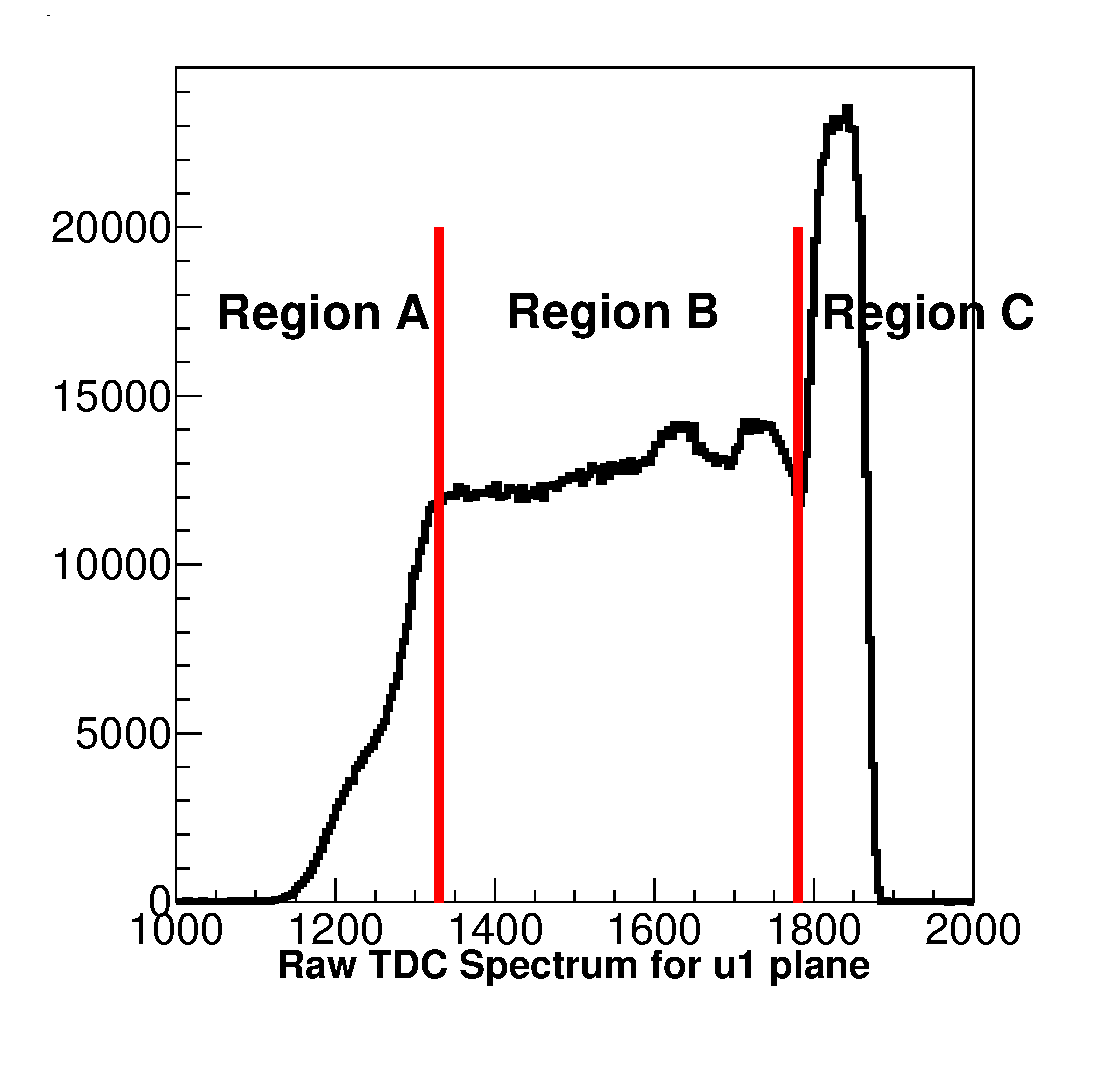
\includegraphics[width=0.4\textwidth] {./vdc_plot/vdc_cali3.eps}
 		\caption{ Raw TDC spectrum for u1 wire plane} \label{vdc_p1}
 	\end{center}
\end{figure}   
\begin{enumerate}
\item Region A: In this region, the fire point is relatively far from the sense fire and the  probability to detect a particle is low 
\item Region B: The events in these area correspond to the area in the wire plane with a uniform electric field, so the probability to detect a particle is uniform
\item Region C: The fire position for these events are very close to the sense wire and the electric field from this area is going to change to radial shape and the probability to detect a particle is going to increase in this area and since the distance from the fire point to the sense wire has a minimum limit so the right side of this area has a sharp slope. 
\end{enumerate}
Since different wire connect to the different TDC Channel and each individual TDC channel has different time offset, the VDC calibration goal is to find out the timing offset for every TDC Channel  and align the timing information in the same way. Usually the reference time is chosen at the sharp slope position of Region C($t_{0}$) as shown in Fig \ref{vdc_p1} and Fig \ref{vdc_p2} shows the offset corrected time at four wire planes after calibration. 
\begin{figure}
 	\begin{center}
 		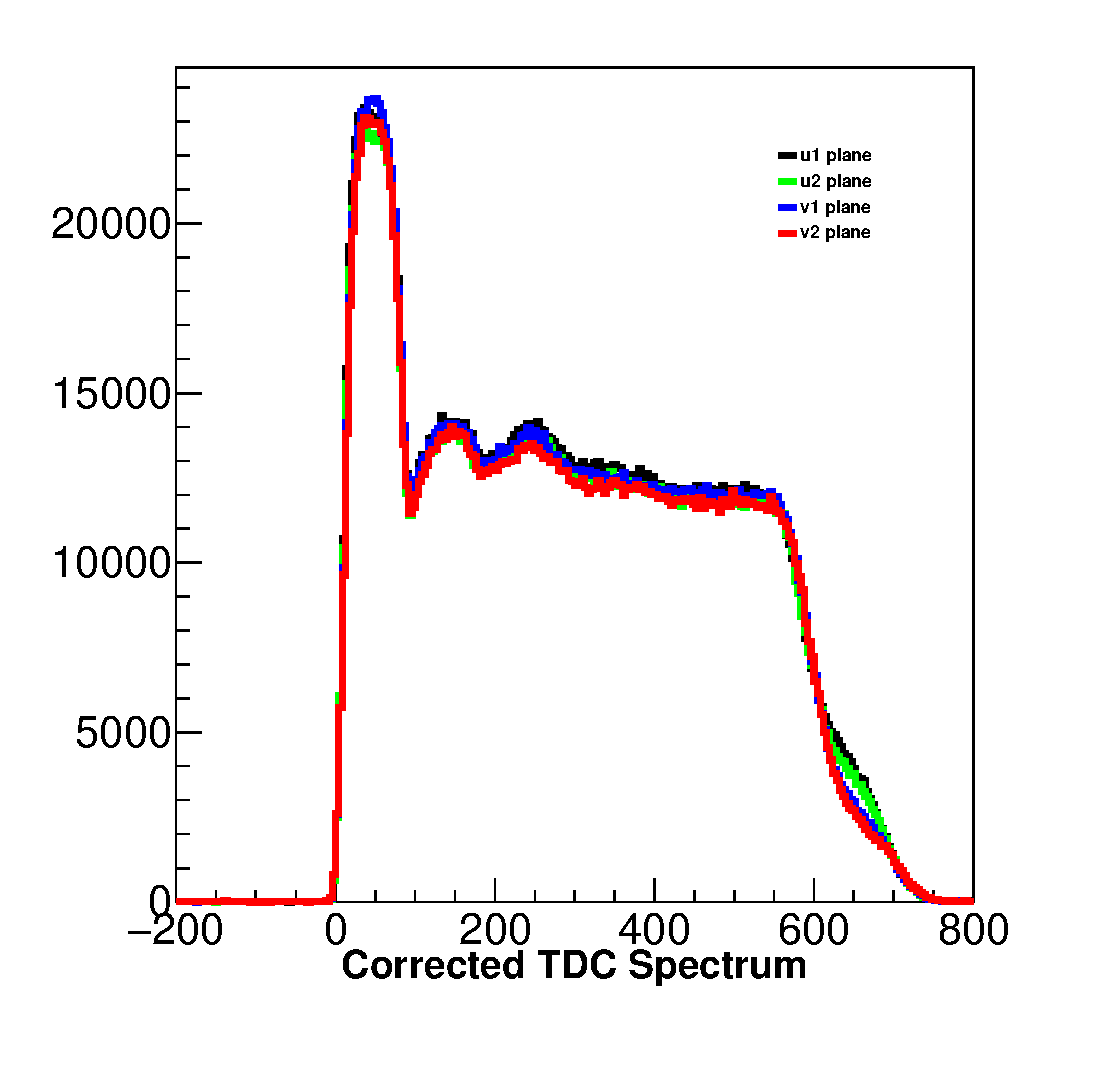
\includegraphics[width=0.4\textwidth] {./vdc_plot/vdc_cali2.eps}
 		\caption{ Corrected TDC spectrum for the 4 wire plane after calibration } \label{vdc_p2}
 	\end{center}
\end{figure}   


 \subsection{iii. BPM}
\subsection{BPM PreBeam Check}




 \subsection{iv. Raster}
 (Tyler Hague)
 The Hall A Raster system was calibrated using a combination of the BPMs, Carbon Hole target, and Carbon Single Foil target. The goal of a successful calibration is to convert the ADC readout of the raster current into a beam position. To do this, a central position of the beam and a conversion factor from ADC readout to beam position deviation from the center.

In Hall A, we have two sets of raster coils working in tandem for the 12 GeV era. These rasters are synced to ensure that they work together, rather than against each other. With this knowledge, the Hall A Analyzer is set up so that the signals from a single raster set are used to determine the beam position. In our case, the analysis code is set up to use the upstream raster coils.

To determine the conversion from ADC to position for the horizontal direction in the hall reference frame (referred to as 'x' from here), we use the Carbon Single Foil Target. When the raster is properly calibrated in the x direction, there should be no correlation between the beam x position and the reconstructed z position of events. To do this, the z position of physics events are sliced in bins of beam x and then fit with a gaussian. The peak position of the each gaussian is then plotted versus the corresponding x position and fit with a line. Doing this method twice with two different preliminary (incorrect) calibrations allows for the slopes to be interpolated to the calibration that would yield no slope (no correlation).

This same procedure can be used with a momentum feature (e.g. the Hydrogen Elastic Peak) to calibrate the vertical direction in the hall reference frame ('y'). However, in the MARATHON kinematics there is no such momentum feature available. As an alternative, the carbon hole is fit to determine the calibration with the knowledge that it is 2mm in diameter. The fit is done using a radial sigmoid function to account for smearing that occurs during reconstruction. A sigmoid is a continuous function that approaches a step function as a "hardness" factor is approaches infinity.

The function used is:
\begin{equation}
\frac{[0]}{1+e^{-[5]*\left(\left([1]*\left([2]-x\right)\right)^{2}+\left([3]*\left([4]-y\right)\right)^{2}-1\right)}}+[6]
\end{equation}

In this function:
\begin{tabular}{l|l}
	\multicolumn{2}{l}{Variable Definitions}
	\hline
	$[0]$ & \\
	$[1]$ & \\
	$[2]$ & \\
	$[3]$ & \\
	$[4]$ & \\
	$[5]$ & \\
	$[6]$ & \\
\end{tabular}

Using the sigmoid fit, we found that the edge determined by the fit (the halfway point on the curve) was incorrect. This was discovered by looking at the correlation between the reconstructed x position of the beam and the reconstructed z of the events. However, we can guess that the "true" edge lies at approximately the same point on the curve in both x and y. Using the known conversion for x from the Carbon Single Foil Target, we can determine the position on the curve of the edge and then slide that along the contour of the sigmoid to determine the edge in y.


 \subsection{v. BCM}
\subsection{Unser and Beam Current Monitors Calibration}
In order to accurately calibrate the BCM's, first the unser must be calibrated. The unser is used as an absolute reference to which the BCM's are calibrated to. The procedure to calibrate the unser involves sending a constant and known currents through a thin wire inside of the unser. A series of currents with, over a range between 2.5 - 100 $\mu$A,during 90 second intervals, as can be seen in figure (??). which shows the frequency response of the unser for the various currents. A linear fit of sent current vs the unser response, determines an overall gain factor for the unser. The gain of the unser of calibrated 4 times during MARATHON before each BCM calibration was preformed, in order to check the unser's stability. Figure(??) shows the unser was stable during the entirety of the MARATHON run. 

\begin{table}[ht]
\caption{Unser Calibration Results}
%\centering
\begin{center}
\begin{tabular}{l| c| c| c| r}
Date & 03-05 & 03-28 & 4-03 & 04-06  \\
\hline
Unser Gain & 2.526e-4 & 2.524e-4 & 2.529e-4 & 2.527e-4\\
\end{tabular}
\end{center}
\end{table}

Having calibrated the unser, we can then calibrate the BCMs in a similar manner to the calibration of the unser but replacing the current from a wire with current from the electron beam. For the BCM calibrations during MARATHON and all Tritium experiments, the range in current was between 3 - 22.5 $\mu$A. Again, the procedure intervals of 90 seconds (i.e 90 seconds of continuous current to the Hall followed by 90 seconds with no beam). 
The Calibration procedure requires making cuts in the frequency response of the unser and BCM receiver and integrating the total amount of frequency to determine the average frequency of the receiver during the given time interval. An example of the cuts made is shown in figure 3

The unser frequency during the calibration can be related to the delivered current using the gain factor determined from the unser calibration. 
\begin{equation}
I_{unser} = gain * f_{unser}
\end{equation}

By then plotting $I_{unser} vs freq_{BCM}$ and fitting with a linear function, the gain and offset (which are proportional the slope and intercept of the fit respectively) of each BCM receiver can be determined. The gain 



%unser
\begin{figure}[H]
\begin{center}
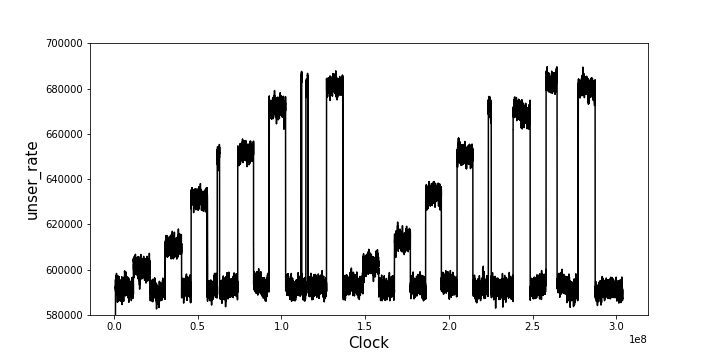
\includegraphics[angle=0, scale =0.65]{Unser_freq.png}
\end{center}
\caption{BCM Calibration : unser}
\end{figure}
%dnew
\begin{figure}[H]
\begin{center}
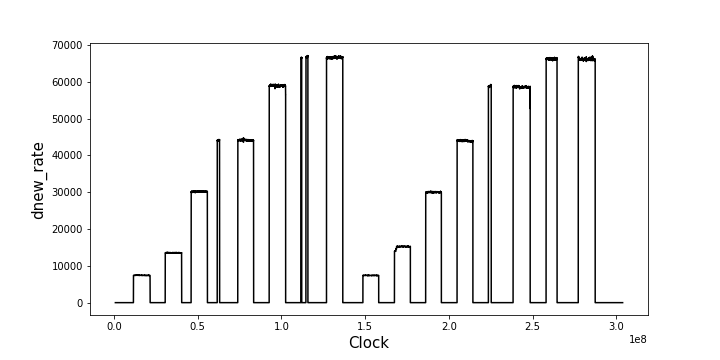
\includegraphics[angle=0, scale =0.65]{Dnew_freq.png}
\end{center}
\caption{BCM Calibration : dnew}
\end{figure}


\begin{figure}[H]
\begin{center}
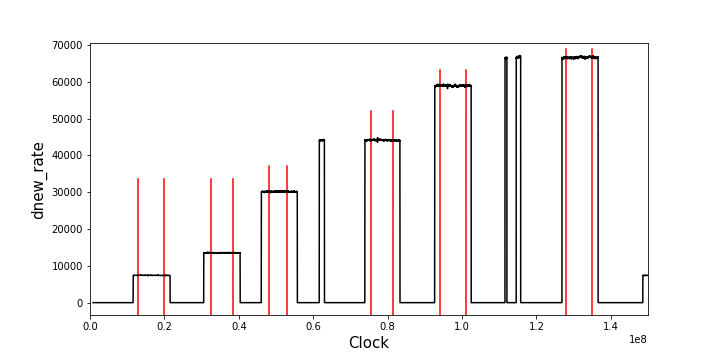
\includegraphics[angle=0, scale =0.65]{Dnew_freq_cuts.png}
\end{center}
\caption{Frequency cuts}
\end{figure}

Table(??) shows the result of the 3 BCM calibrations for the dnew digital BCM receiver.
\begin{table}[ht]
\caption{BCM Calibration Results}
%\centering
\begin{center}
\begin{tabular}{l| c| c| r}
   & 03-05 & 03-28 & 4-03 \\
\hline
dnew Gain & 3.3358e-4 & 3.3351e-4 & 3.3372e-4\\
\hline
dnew offset & -0.097  &   0.003   & 0.132         \\
\end{tabular}
\end{center}
\end{table}


 
 \subsection{vi. Optics}
 (Tong Su)
 The scattering particle track from focal plane need to be reconstructed to the target before bended by the spectrometer magnets to determine the scattering vertex, scattering angle and momentum. To do this , a magnet optics matrix need to be well calibrated.
\section{Corrdinate system}
There are two coordinate system are important for the reconstructed variable: The Hall Coordinate System(HCS) and the Target Coordinate System(TCS). The origin of the HCS is at the Hall center.  Z axis direction is alone the beam line and point to the beam dump and y axis is point horizontally up. Each HRS also has its own TCS(Fig \ref{optics_plt1} . The z axis of the TCS is along the center ray of the spectrometer and the x axis is horizontally pointing down. The original of the TCS is at a constant distance   $L$ in front of the HRS entrance and this distance is defined with the distance from Hall center to the HRS entrance under the ideal situation which means the all the spectrometer offsets are zero. According to this definition, we can see that under the ideal case, the origin of the TCS can match the origin of the HCS. The trajectory of the scattering particle can be reocnstructed to the target described by 4 variables in the TCS: the position in the no dispersive plane($y_{tg}$), the angles in the dispersive direction(out-of-plan, $\theta_{tg}$) and the non-dispersive direction(in-plane, $\phi_{tg}$) and the relative momentum $\delta=(p-p_{0})/p_{0}$, where the $p$ is the momentum for the scattering momentum and $p_{0}$ is the setting momentum of the HRS.
\begin{figure}
 	\begin{center}
 		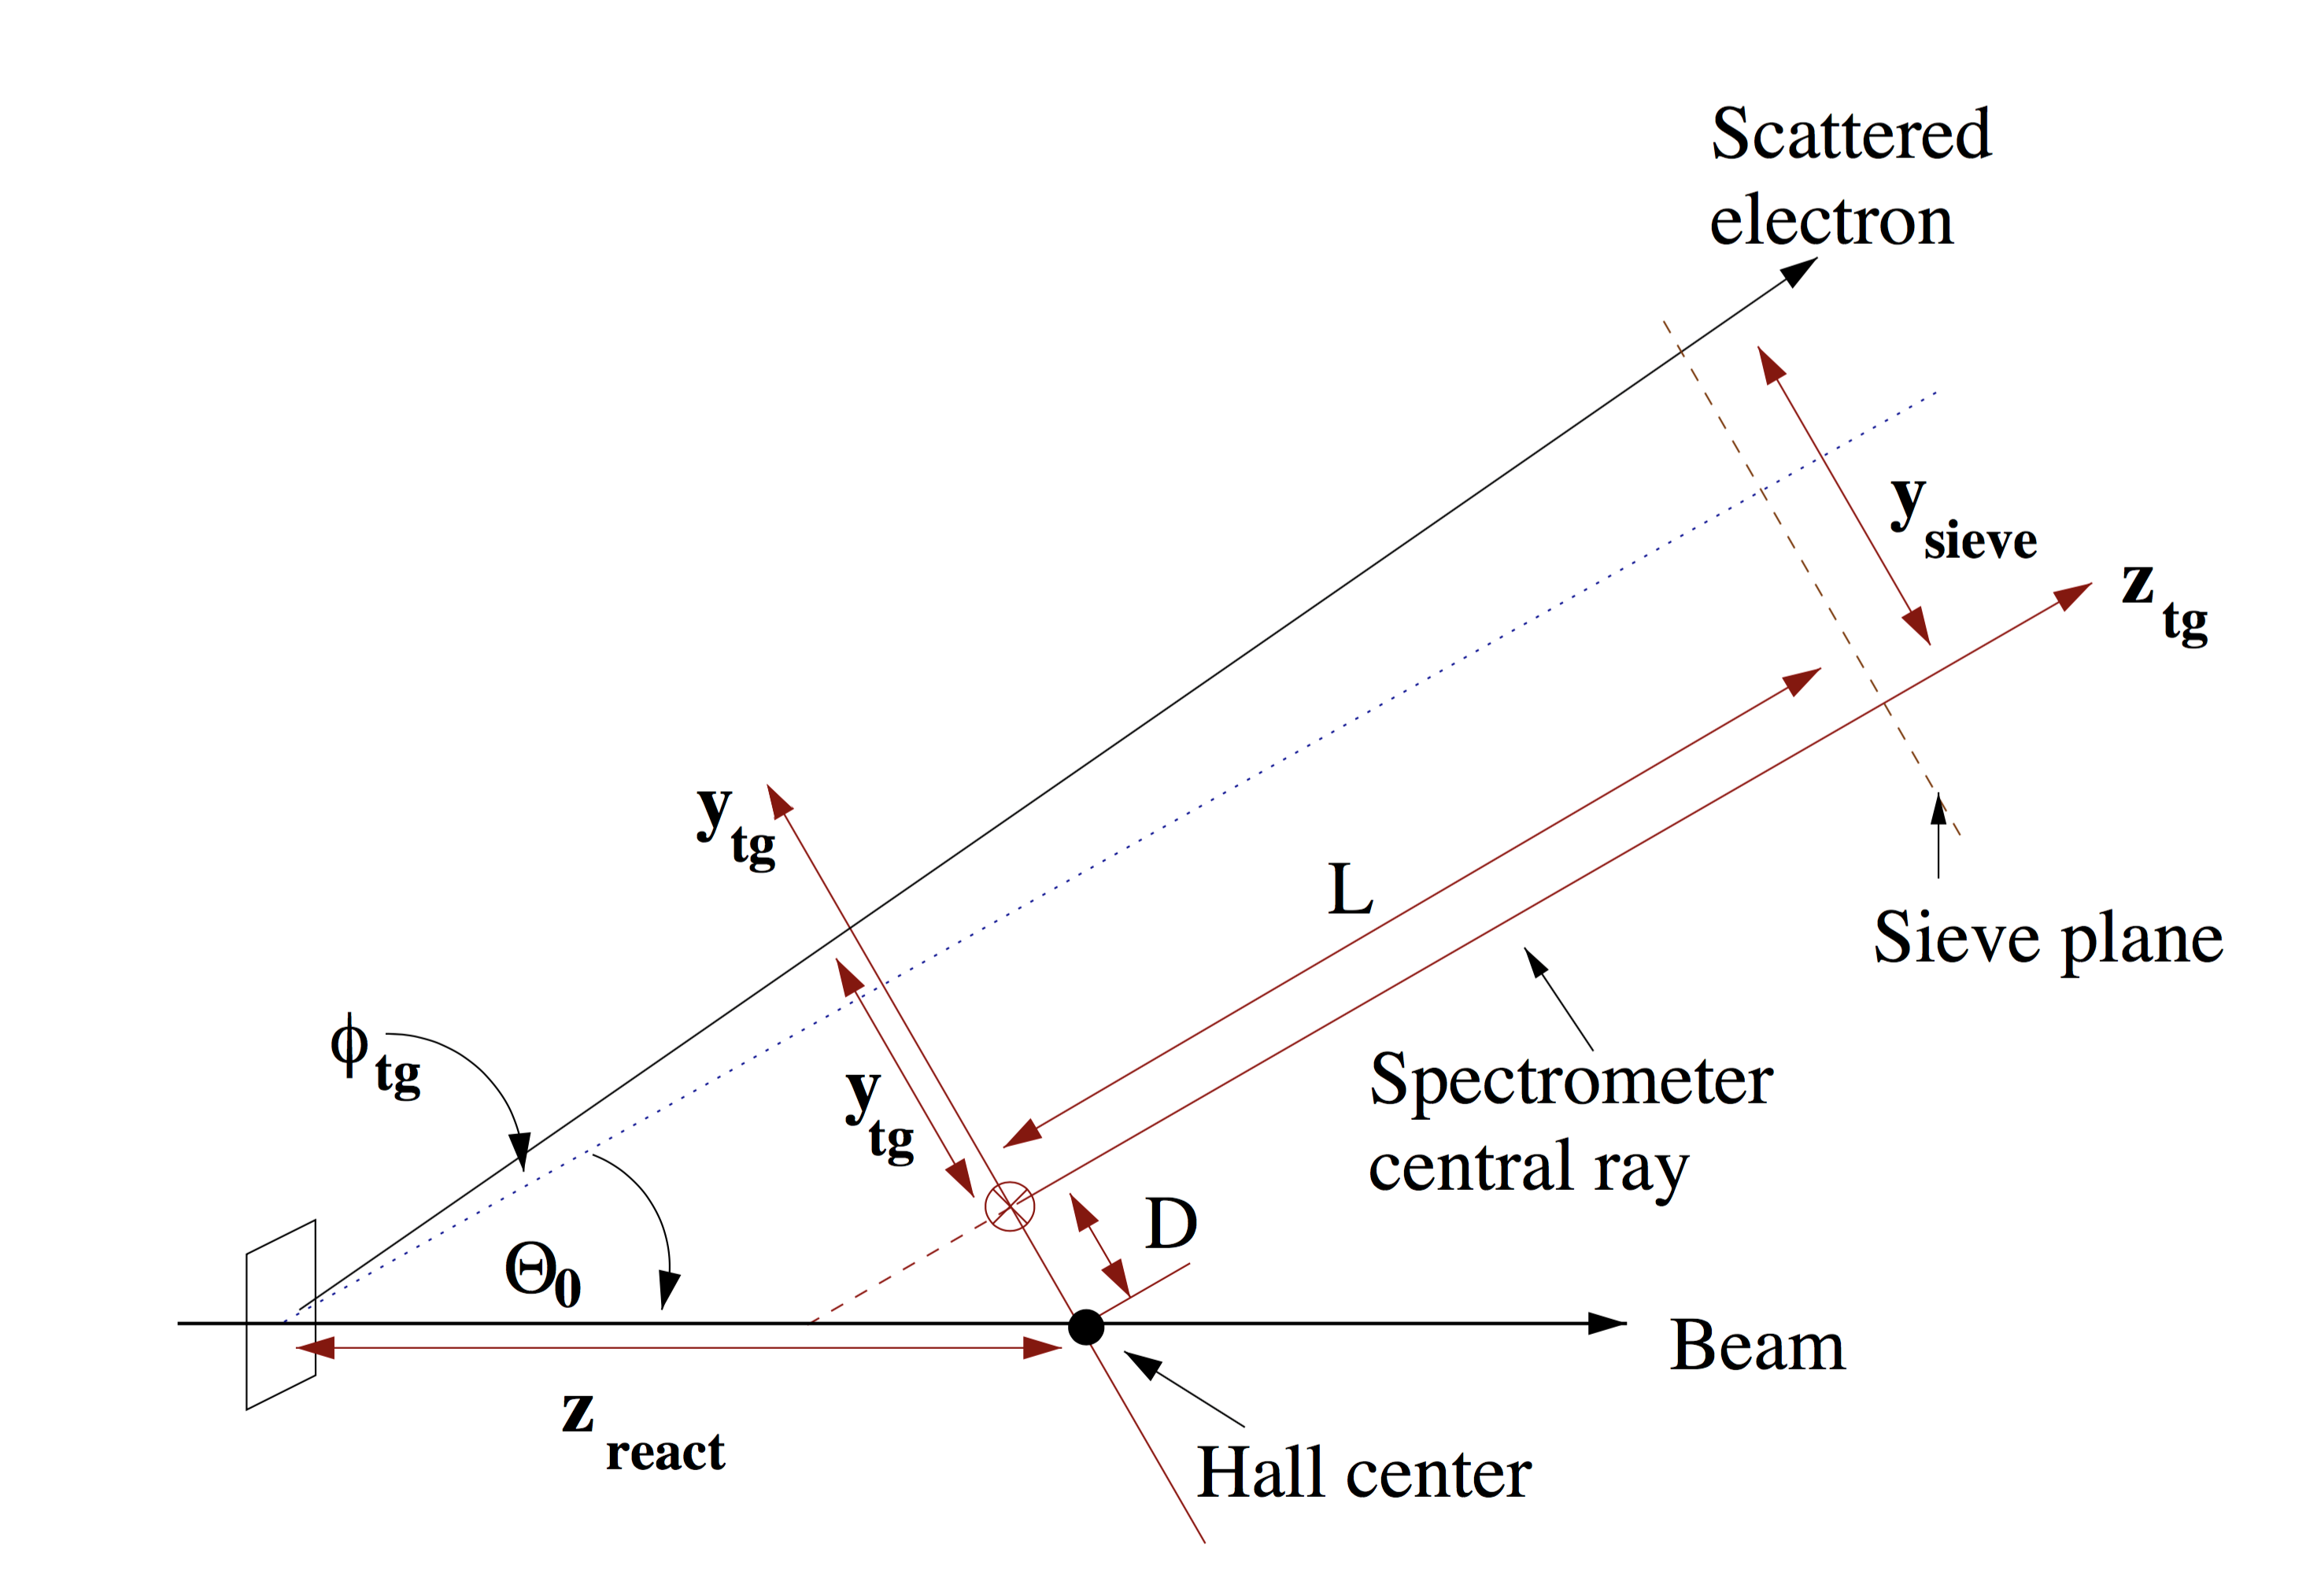
\includegraphics[width=0.2\textwidth] {./optics_plot/optics_4.png}
 		\caption{The schematic plot of the TCS from RefXXX, in which D stands for the spectrmoeter offset from the hall center } \label{optics_plt1}
 	\end{center}
\end{figure}   



The relations between the 4 traking variables in the focal plane and the 4 reconstrcuted variables at TCS can be described as a set of the following polynomials:
\begin{equation}  
\left\{  
             \begin{array}{lr}  
             y_{tg}=\sum_{jkl}Y_{jkl} \theta_{fp}^{j} y_{fp}^{k} \phi_{fp}^{l} \\  
             \theta_{tg}=\sum_{jkl}T_{jkl} \theta_{fp}^{j} y_{fp}^{k} \phi_{fp}^{l} \\    
             \phi_{tg}=\sum_{jkl}P_{jkl} \theta_{fp}^{j} y_{fp}^{k} \phi_{fp}^{l} \\     
             \delta_{tg}=\sum_{jkl}D_{jkl} \theta_{fp}^{j} y_{fp}^{k} \phi_{fp}^{l}\\  
             \end{array}  
\right.  
\label{optics_1}
\end{equation}  
where the 4 sets of cofficients are the function of $x_{fp}$:
\begin{equation}  
\left\{  
             \begin{array}{lr}  
             Y_{jkl}=\sum_{i=0}^{m} C_{ijkl}^{Y} x_{fp}^{i} \\  
             T_{jkl}=\sum_{i=0}^{m} C_{ijkl}^{T} x_{fp}^{i} \\
             P_{jkl}=\sum_{i=0}^{m} C_{ijkl}^{P} x_{fp}^{i} \\
             D_{jkl}=\sum_{i=0}^{m} C_{ijkl}^{D} x_{fp}^{i} \\ 
             \end{array}  
\right.  
\label{optics_2 }
\end{equation} 
The four sets of cofficients $C_{ijkl}^{Y/T/P/D}$ describe the optics properties of the spectrometer magnets and the above four sets of polynmoinal also called the HRS optics matrix.                                                                     
\section{Optics Data Taking and Optimized Procedure }
The so-called optics calibration is that to determine the cofficients described in Eq \ref{optics_2 }. In order to reach this goal, some desigined data need to be taking during druring the experiment. Since the 4 sets of the matrice are independent mathematically, in principle, we can use different sets of data to calibrate different target variable . Experimentally, $C^{Y}$, $C^{T}$ and $C^{P}$ use one set of the data which is expected can cover the spectrometer acceptance as much as it can and for inclusive experiment, $C_{P}$ can only choose the kinematics setting with the well known scattering momentum such as the elastic scattering data. To label the spatial variables in the TCS, a mutifoil target (Fig \ref{optics_plt2} ) and a sieve-slit collimator (Fig \ref{optics_plt3})  are used for the optics calibration data. For Tritium Experiment, the mutifoil target is consisted of 11 carbon foil which are evenlty arranged along the beam direction. The distance between the two adjacent foils is 2.5cm and the total length of the mutifoil target is 25cm which is equivalent to the gas target length. The sieve-slit collimater tritium used is the new desgined one from the GMP experiment which is make of tungsten with 1in thickness. Electrons will lose enough energy   by passing through the tungsten, so that only electrons go throught the hole can reach the focal plane.  In addition, a complete and percise survey which including the postion of the spectrometer, target and sieve-slit also import to label data correctly. Not only that, a well understanded beam positon from a calibrated BPMs also to do the optics calibration.

\begin{figure}
 	\begin{center}
 		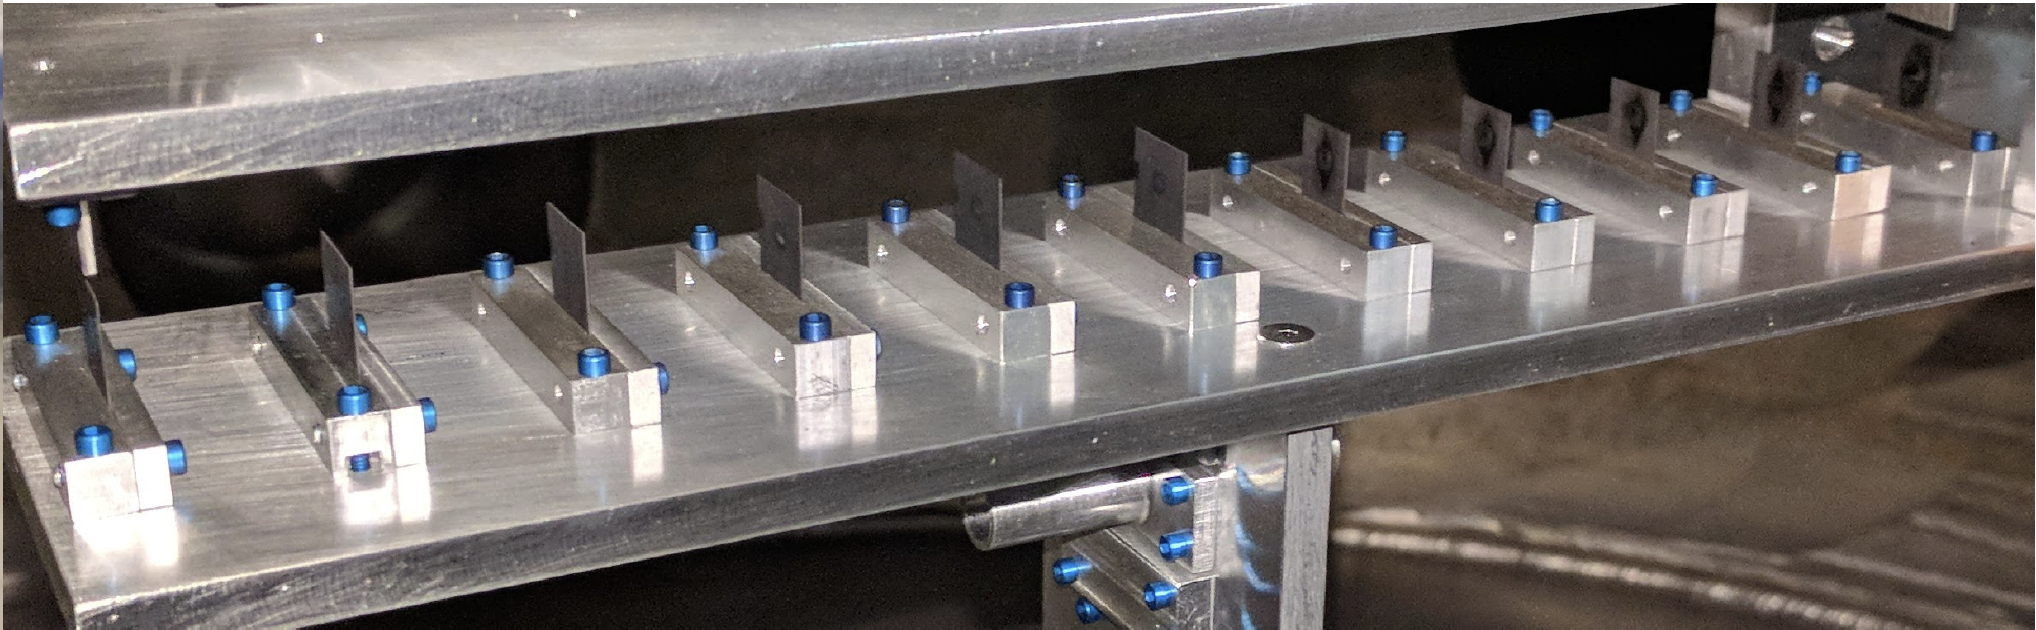
\includegraphics[width=0.2\textwidth] {./optics_plot/optics_3.png}
 		\caption{Mutifoil Target for Tritium Experiment: 11 carbon foil totally which can cover the full 25cm target length} \label{optics_plt2}
 	\end{center}
\end{figure}   

\begin{figure}
 	\begin{center}
 		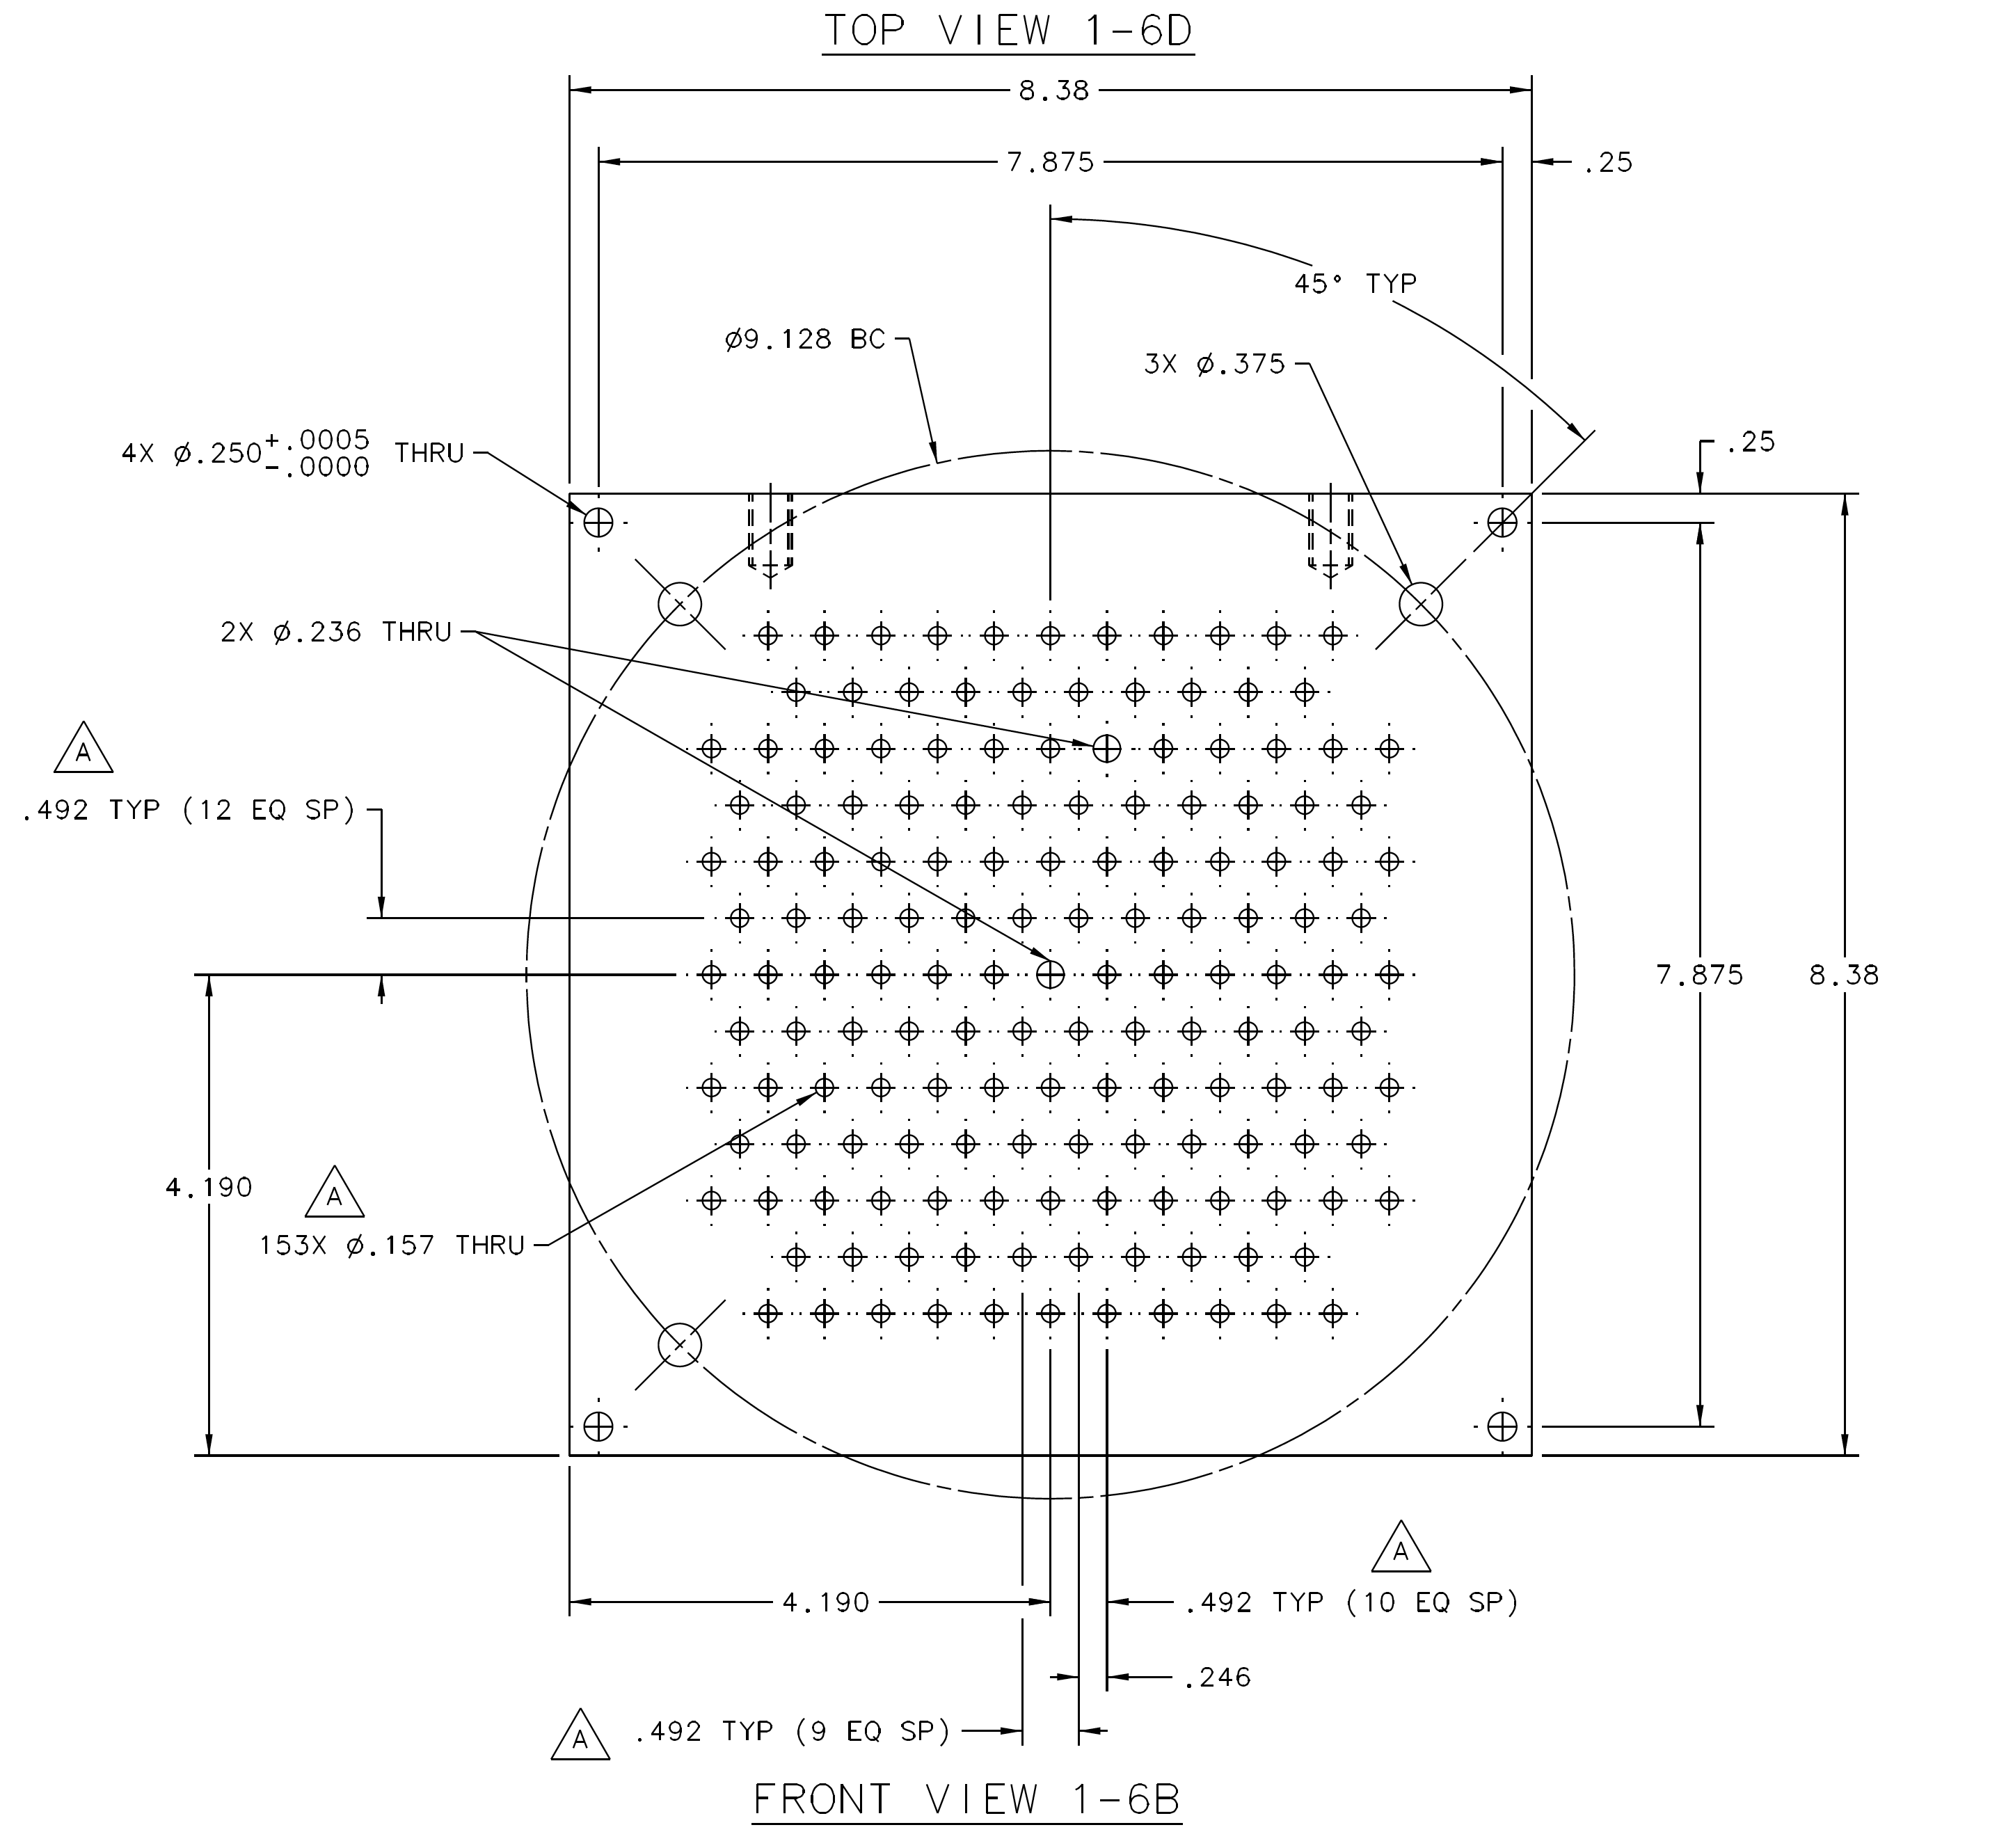
\includegraphics[width=0.2\textwidth] {./optics_plot/optics_1.png}
 		\caption{Engineering schematic plot for sieve-slit collimator used for Tritium Experiment } \label{optics_plt3}
 	\end{center}
\end{figure}   
For the three spatial target variable optimization, firstly, good events need to be selected by apply the general good electron cut and then for each selected event, which foil it is scattered from the target($Foil\_id$) and which hole it passes through the 
sleve-silt($Holel\_id$) need to be discriminated. Combining with all the positions mentioned above, the really target variable $y_{tg}^{REAL}$, $\theta_{tg}^{REAL}$ and $\phi_{tg}^{REAL}$ can be calculated by the geometrical relationships. On the other side, from the initial optics matrix which usually comes from the pervious experiment the reconstructed target variables: $y_{tg}^{RCON}$, $\theta_{tg}^{RCON}$ and $\phi_{tg}^{RCON}$ can be obtained. Then the optics matrix elements can be optimized by minimizing the following aberration funtion:
\begin{equation}  
\Delta(O)=\sum_{events}\left( O^{RECON}-O^{REAL}\right) ^{2}
\end{equation} \label{optics_3}  
Where $O$ stands the $y_{tg}$, $\theta_{tg}$ and $\phi_{tg}$ 

The momentum optimization is similar. After selecting out the elastic scattering events, for each event , the $\delta_{tg}^{RCON}$ and $\delta_{tg}^{REAL}$ can be obtained and optics matrix elements can be optimized by the Eq \ref{optics_3}. But usually to precisely determined the scattering momentum, several corrections need to be applied such as a variety of the energy loss and the elastic peak shift within the spectrometer acceptance. 


\section{Result}
For MARATHON experiment, all the production data was taken at spring,2018  when the HRS magnets tuning was exactly same with the previous GMP experiment so that our magnets optics is also same with the GMP one.  We keep using the GMP most updated optics matrix for both HRS and base on our online check no obvious abnormity found for that GMP optics matrix

MARATHON also use some data about target density study (Boiling effect) taken at Fall,2017. This data used a slliently different tuning than the GMP experiment. Therefore optics for that part of data is analyzed . Since only optics data related to the spatial variable was taken so only $y_{tg}$, $\theta_{tg}$ and $\phi_{tg}$ are optimized and some reault are shown in the Fig \ref{optics_plt4}, Fig \ref{optics_plt5} and Fig \ref{optics_plt6}


\begin{figure}[htbp]
\subfigure[before calibration]{
\begin{minipage}[t]{1\linewidth}
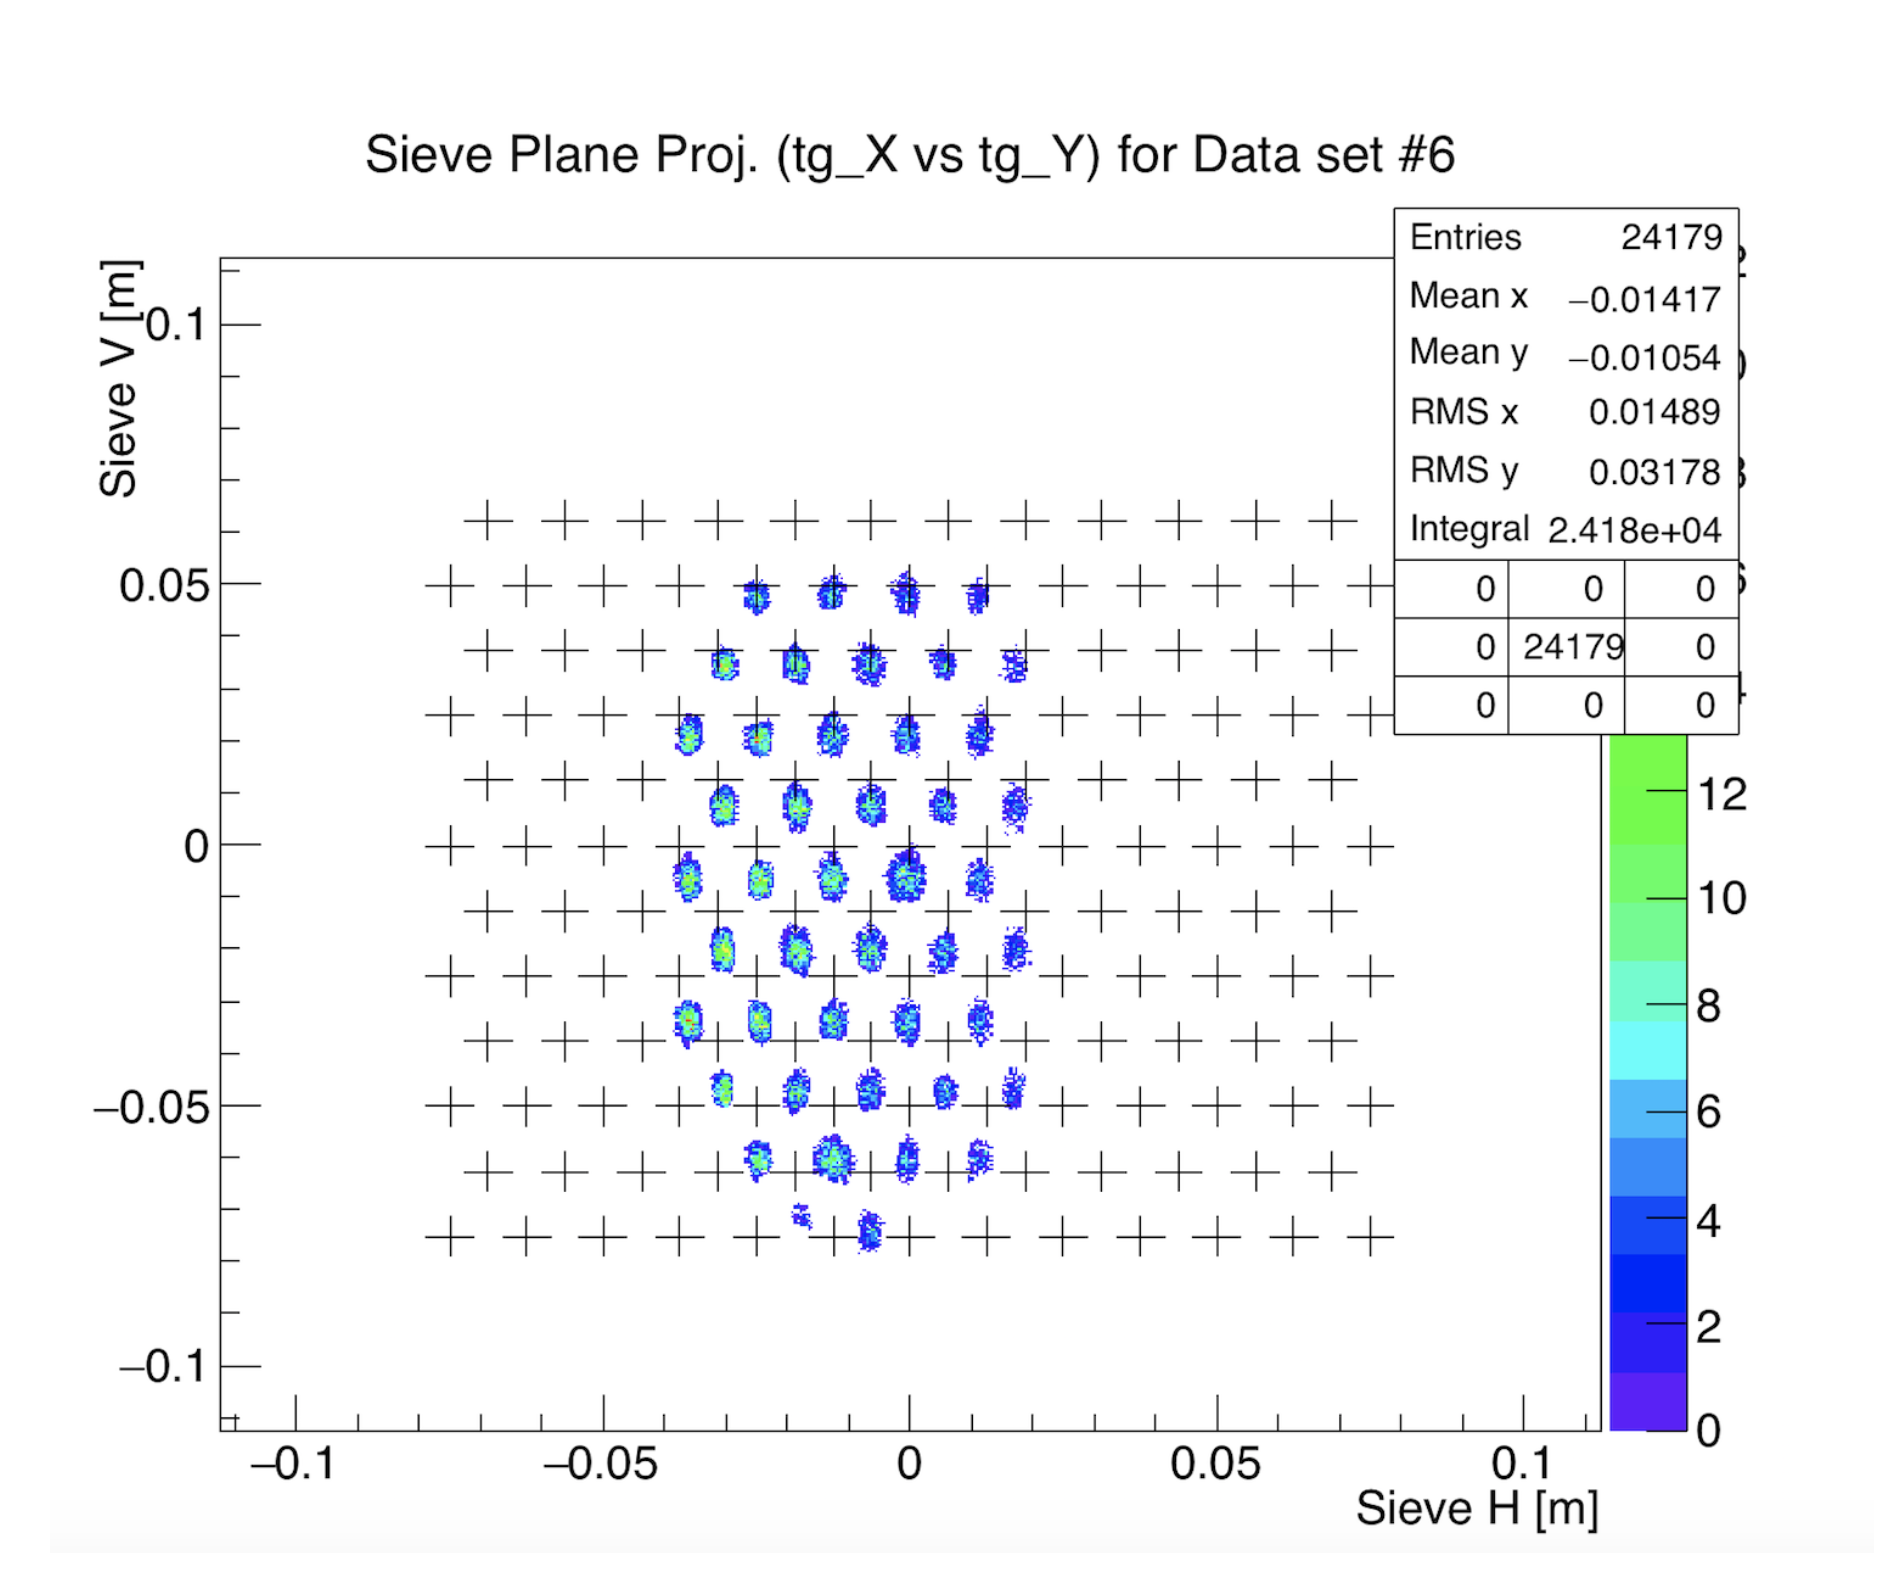
\includegraphics[width=3in]{./optics_plot/optics_6.png}
\end{minipage}
}\\
\subfigure[after calibration]{
\begin{minipage}[t]{1\linewidth}
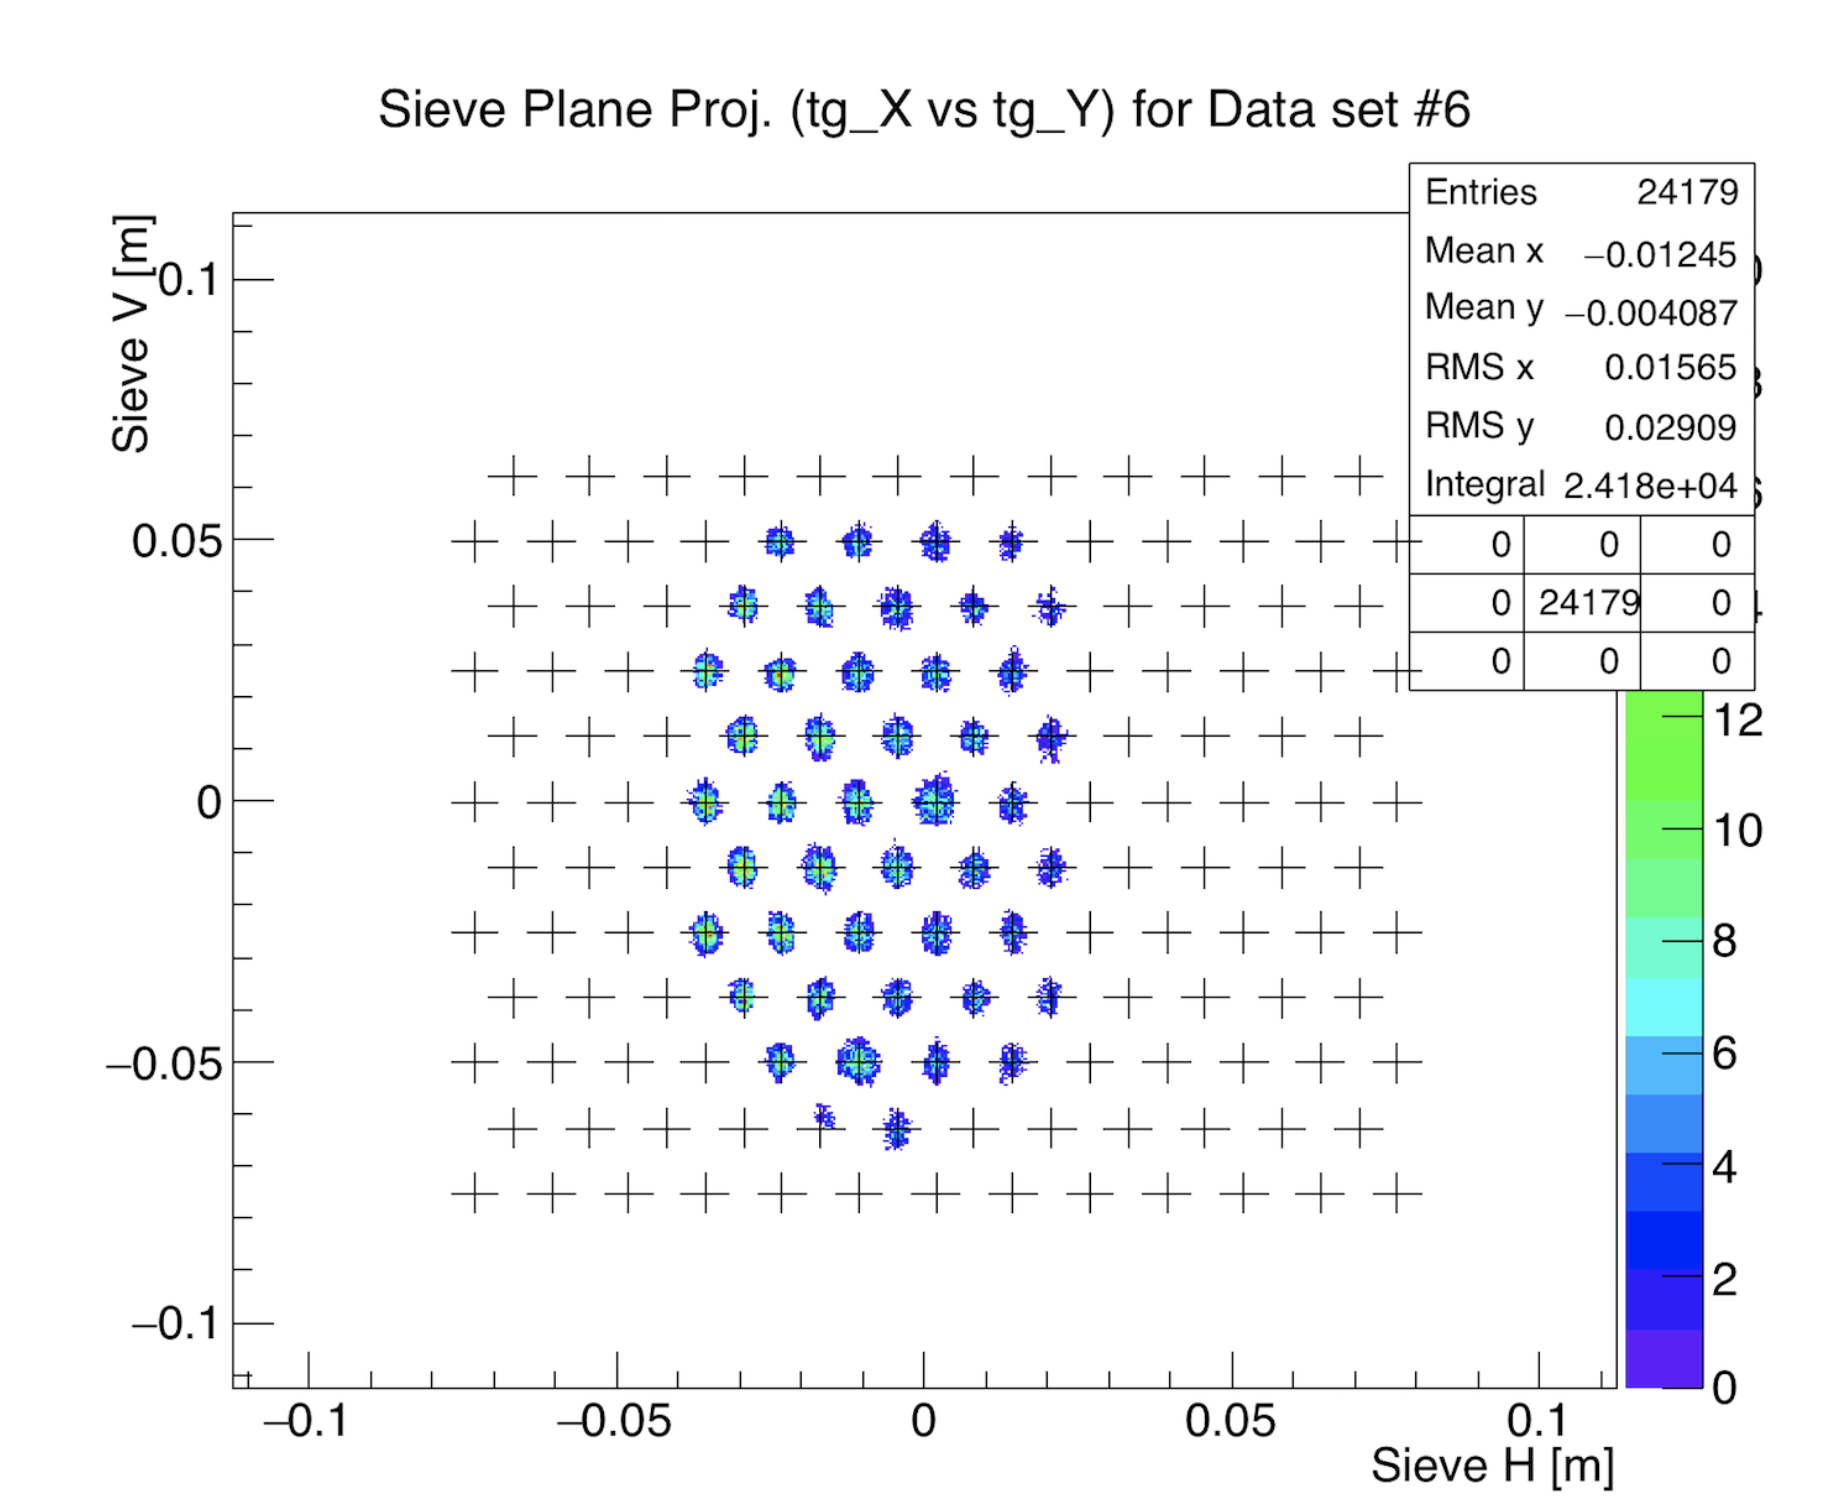
\includegraphics[width=3in]{./optics_plot/optics_5.png}
\end{minipage}
}
 \centering
\caption{$\theta_{tg} $ and $\phi_{tg}$ calibration for the fall,2017 data}
\label{optics_plt4}
\end{figure}

\begin{figure}[htbp]
\subfigure[before calibration]{
\begin{minipage}[t]{1\linewidth}
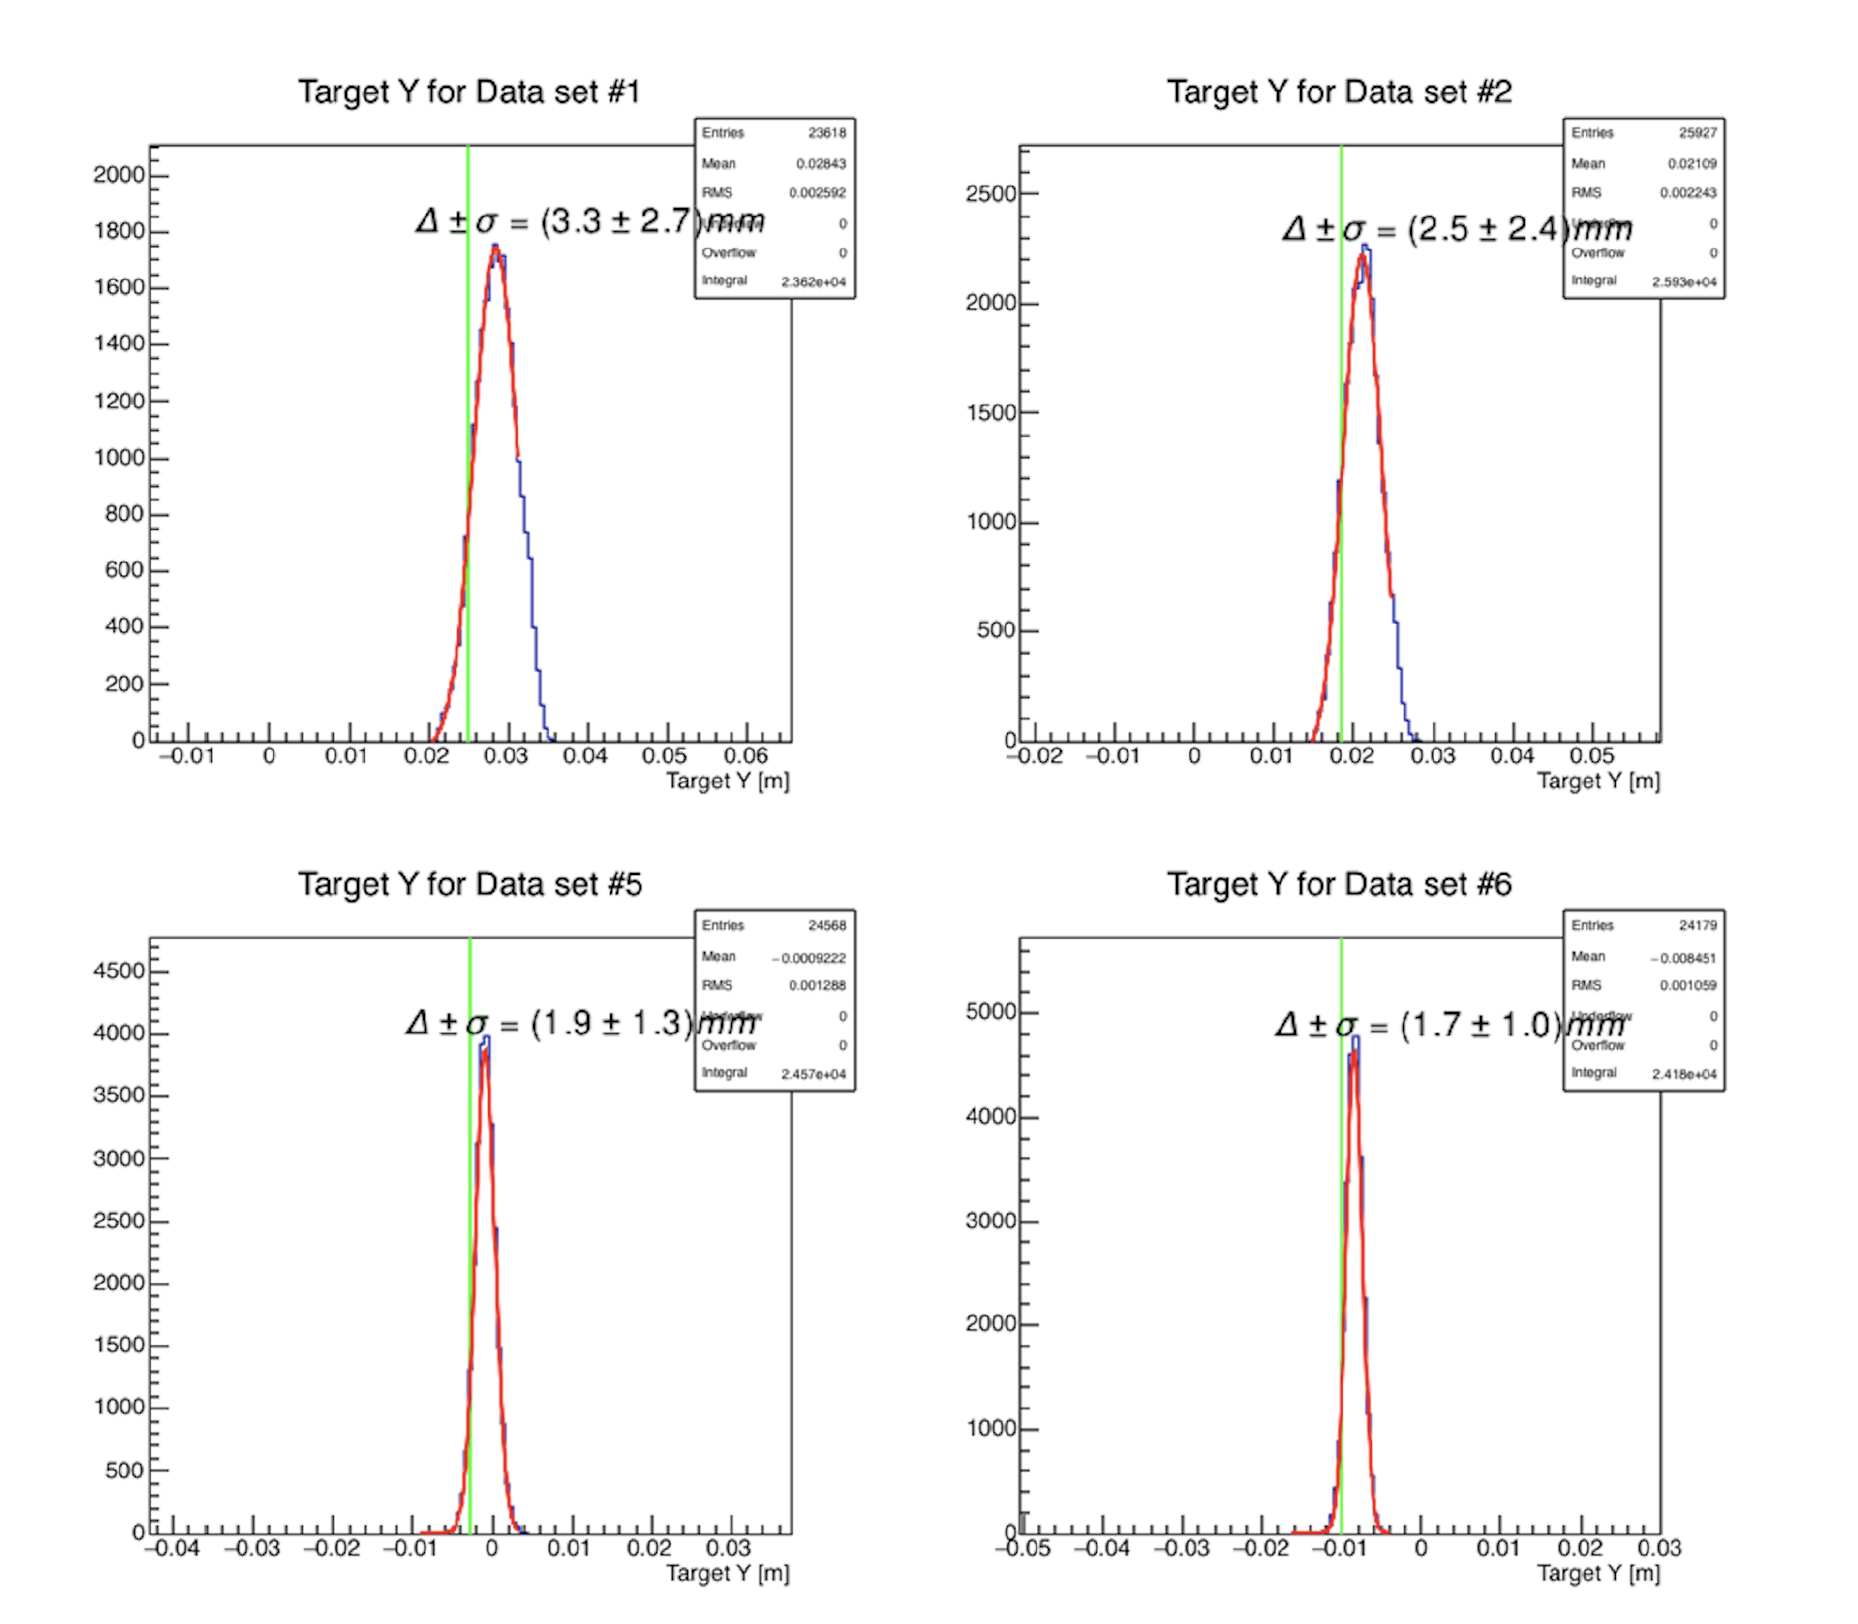
\includegraphics[width=3in]{./optics_plot/optics_8.png}
\end{minipage}
}\\
\subfigure[after calibration]{
\begin{minipage}[t]{1\linewidth}
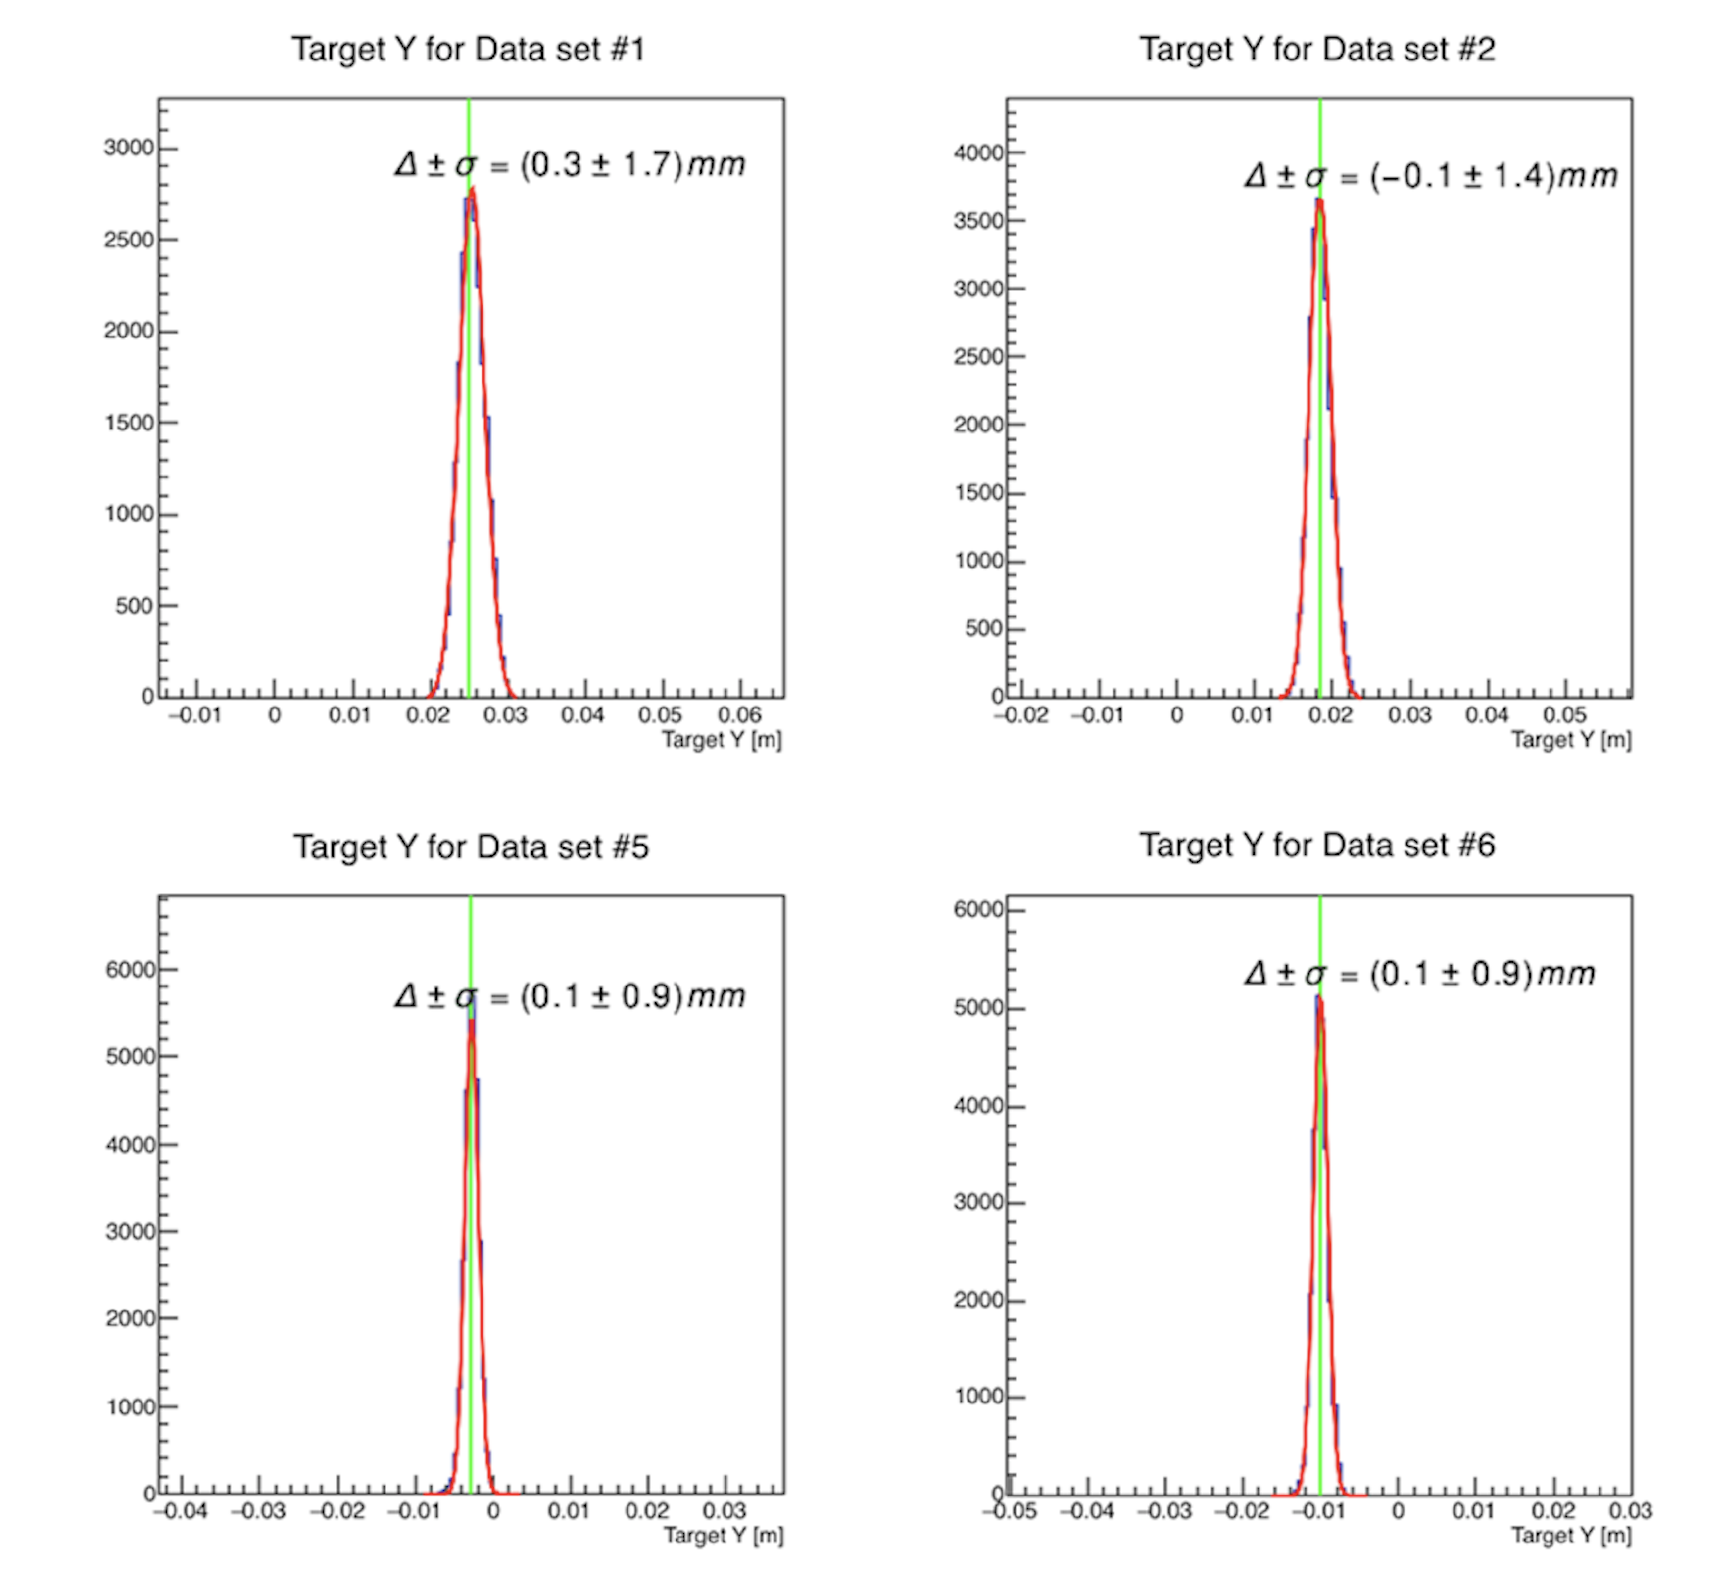
\includegraphics[width=3in]{./optics_plot/optics_7.png}
\end{minipage}
}
 \centering
\caption{$y_{tg}$ calibration for the fall,2017 data}
\label{optics_plt5}
\end{figure}

\begin{figure}
 	\begin{center}
 		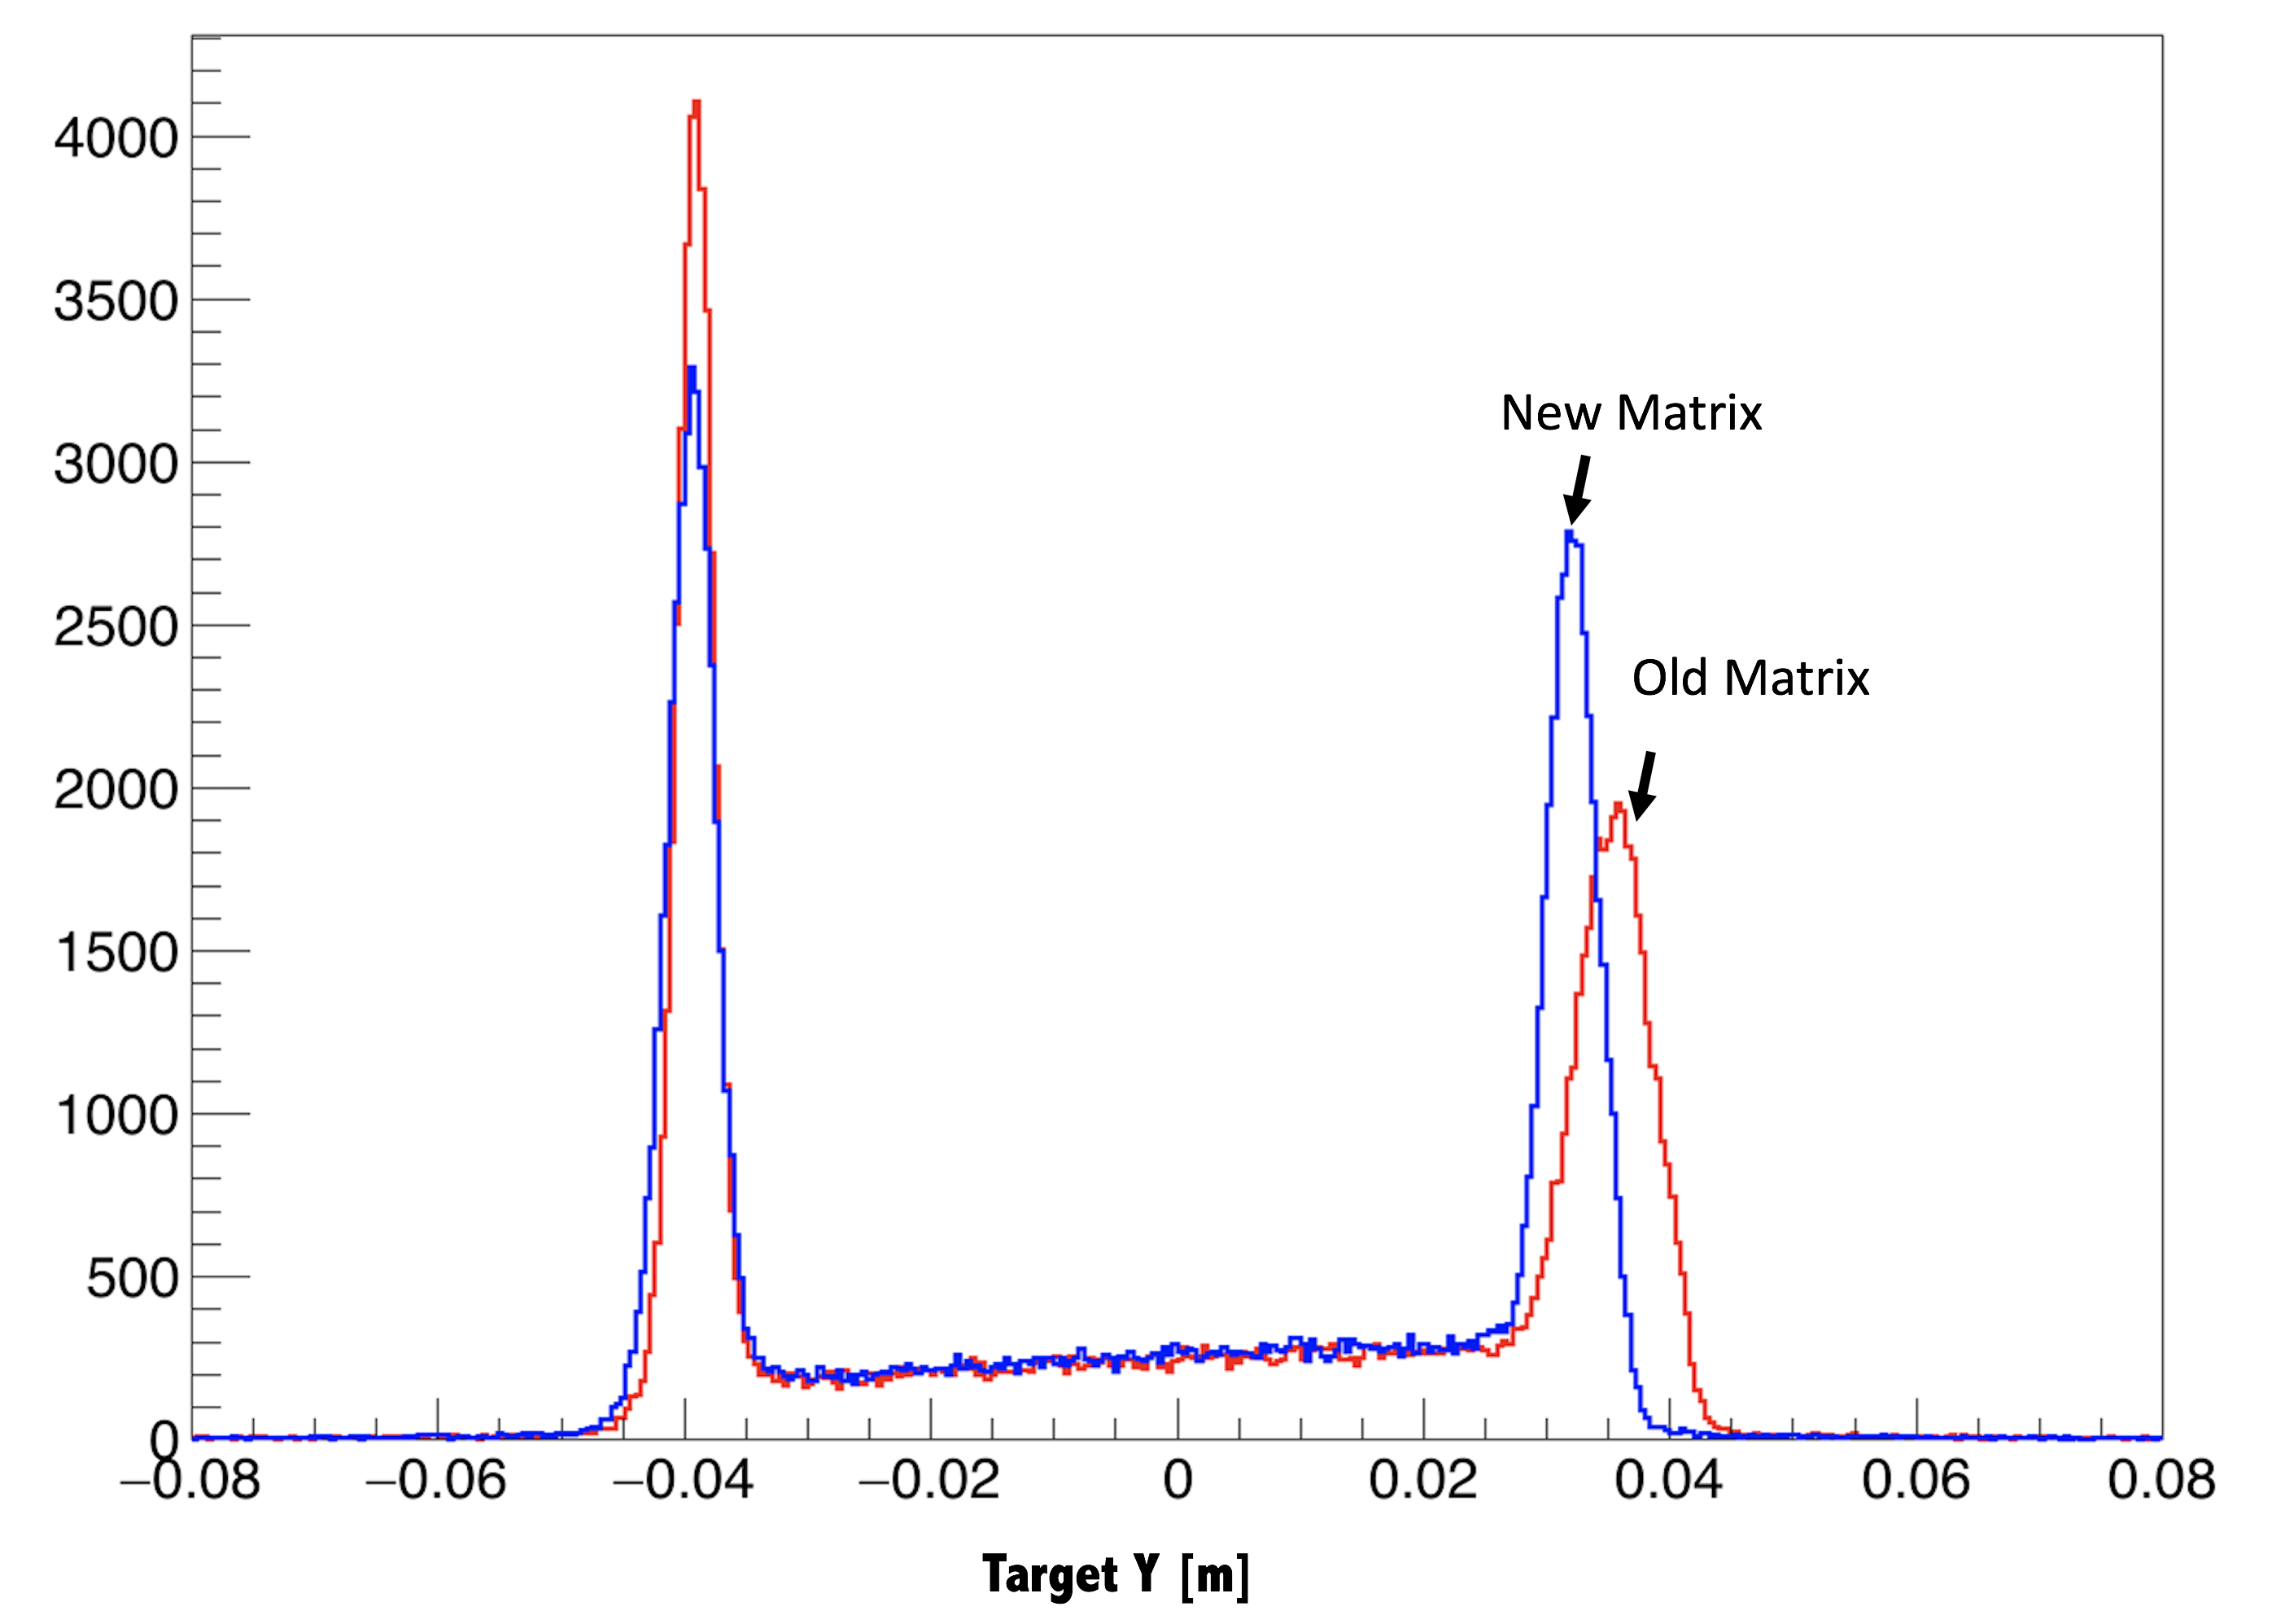
\includegraphics[width=0.3\textwidth] {./optics_plot/optics_2.png}
 		\caption{$y_{tg}$ reconstruction before and after optimize the optice matrix, as we can see , the upstream endcap resolution become better} \label{optics_plt6}
 	\end{center}
\end{figure}   


\section{IV. Corrections}

 \subsection{i. PID}
 (Tong Su)
 


%opening

\section{The Traditional PID Efficiency Study and MARATHON PID Difficulty}
Each arm of the HRS has two particle identification: Gas Cherenkov and Lead Glass calorimeter. Compare to the other hadrons, both of these two detectors are much more sensitive to the electrons and their PID performance is independent. In the analysis, we use these two features by applying a cut on the calibrated Cherenkov ADC sum signals and calorimeter energy (or E/P) signals to distinguish the electrons and not only that these two features can also provide us a way to check the efficiency of these two PID cuts. The tradition way \cite{pid_eff} to check the PID cut efficiency is to apply a tight cut on one of the PID detectors to select a pure electron(pion) sample and check their performance on the other detectors . The electron(pion) efficiency for the checking cut can caculated by:
\begin{equation}\label{pid_eq1}
\epsilon_{pid-cut}=\dfrac{N'}{N_{sample}}
\end{equation}  
Where the $N_{sample}$ is number of events in the selecting sample and the $N'$ is the number of the events can pass the checking cut in the selecting sample.

For MARATHON experiment, we notice that except the traditional background signals which are inseneitive for both PID detectors(X2), there is another kind “particle” (X1) can introduce a large signal in the gas Cherenkov detector which behaves very similar to electron in the Cherenkov but can barely fire the calorimeter which is clearly different than what we expected electron performance in it(Shown in the Fig \ref{pid1}).
\begin{figure}[htbp]

\subfigure[kin1]{
\begin{minipage}[t]{1\linewidth}
\centering
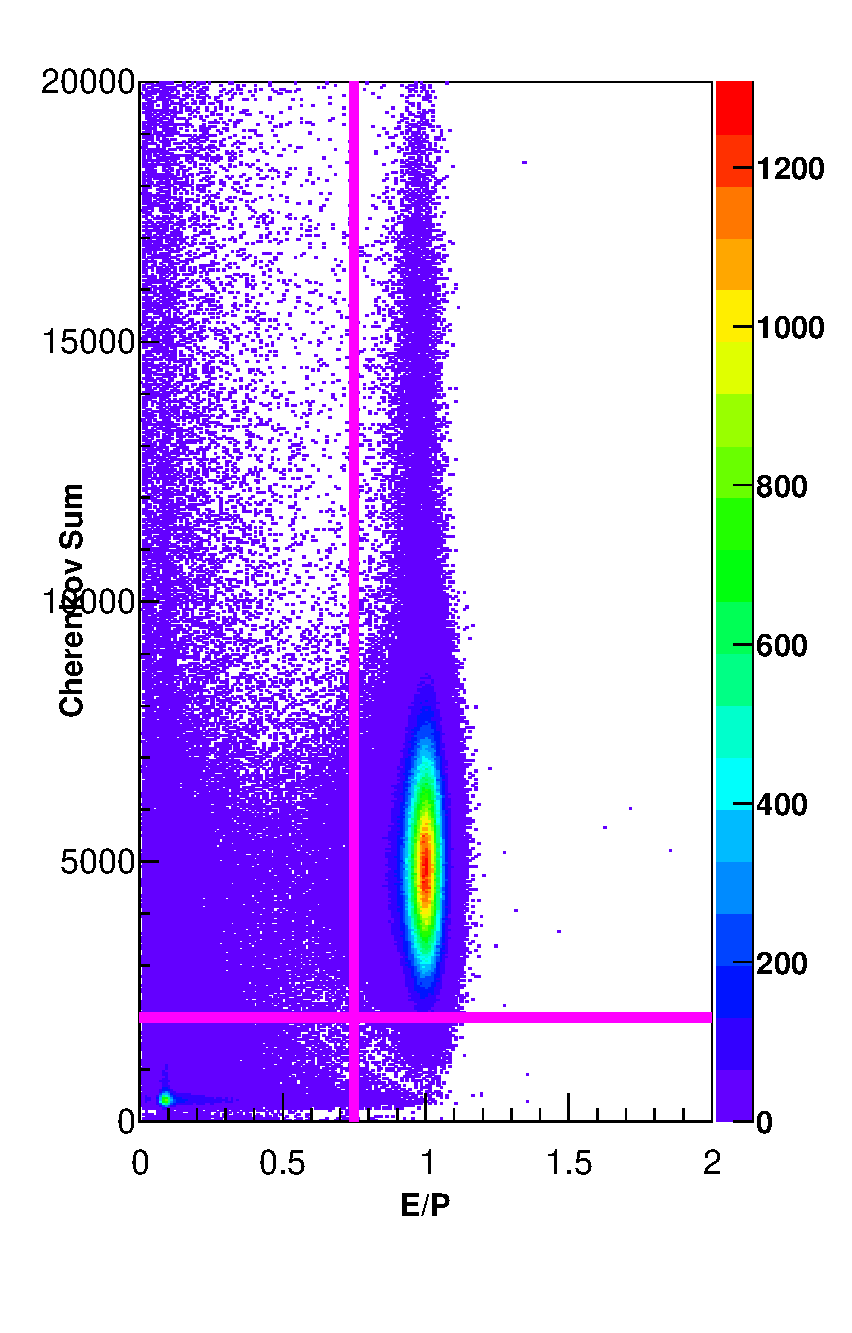
\includegraphics[width=2in]{./pid_plot/pid1.eps}
\end{minipage}
}\\
\centering
\subfigure[kin15]{
\begin{minipage}[t]{1\linewidth}
\centering
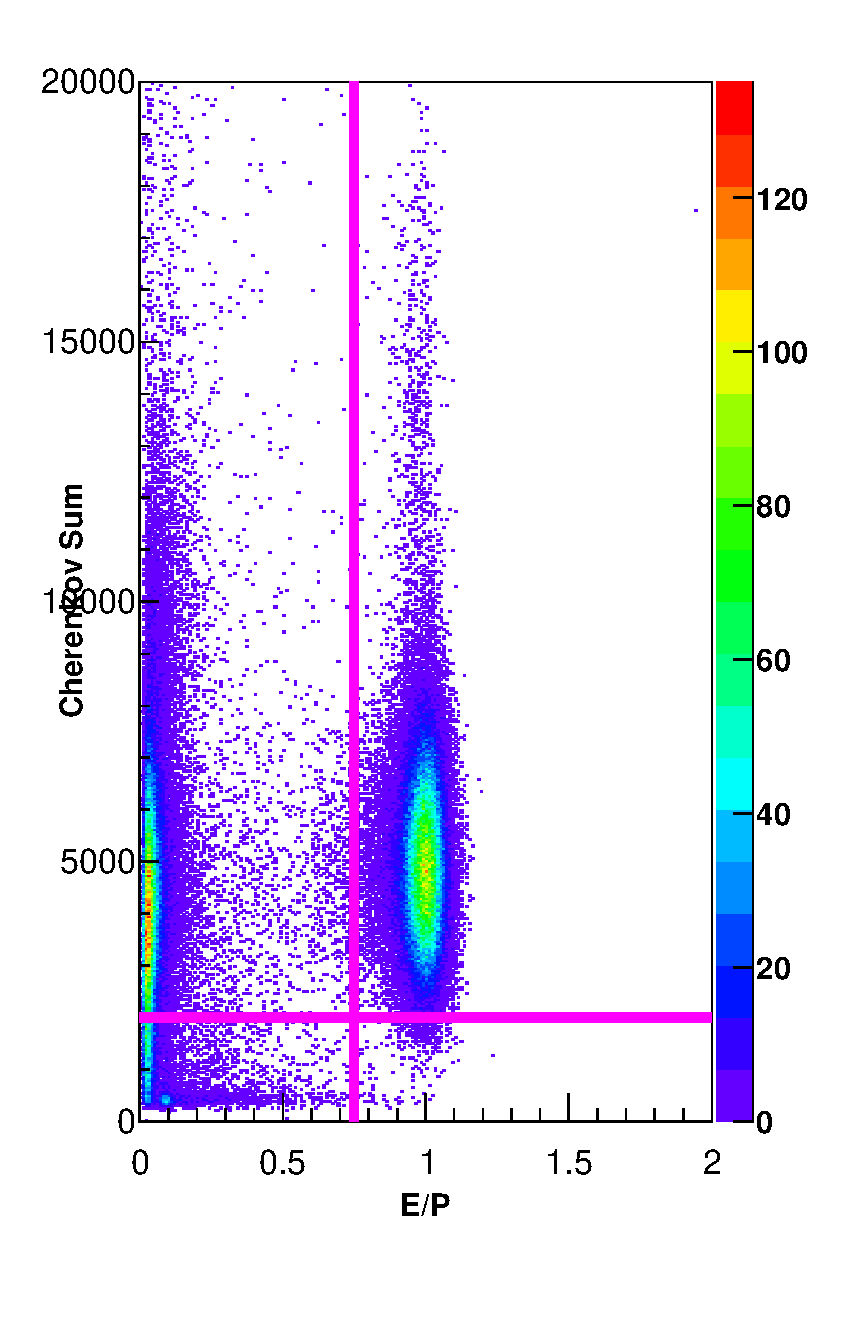
\includegraphics[width=2in]{./pid_plot/pid2.eps}
\end{minipage}
}
\centering
\caption{The 2 PID detector performance for $^{3}H$ at two differnet kinematics setting. General acceptance cut, T2 trigger cut, single track cut and a postive beta cut applied. The two magenta lines indicate the two cut postions for the Cherenkov(horizontal,2000) and E/P(vertical 0.7).  As we can see, different kinematics the ratio of X1 and X2 are different}
\label{pid1}
\end{figure}
The possible explanations for these suspicious signals including 1) for 11 GeV scattering, the high energy neutral particles hitting the back of the HRS dipole and getting into the acceptance and 2) the muon from $\pi^{0}$ decay can have chance to get into the acceptance and have chance to introduce big signal in the Cherenkov. To identify what exactly these signals are still need some work but because of the existence of these signals, there will be a challenge to use the traditional way to check the PID cut efficiency since the as shown in the Table \ref{sample1}, almost no clean sample can be selected out. 
\begin{table}[!ht]
\large
\centering
 \caption{Possibility to cut a pure sample from individual PID detectors}\label{tab:tablenotes}
\begin{threeparttable}
\begin{tabular}[t]{|c|c|c|}\hline
  Experimental Settings & Cherenkov & Calorimeter  \\ \hline        
  electron          &   $\times$ & $\surd$ \\ \hline
  X1                 &  $\times$  & difficult \\  \hline
 X2                  & $\times$  &   difficult\\  \hline  

 \end{tabular}
\begin{tablenotes}
\centering
        \item[1]  $ \times $ means "No", $ \surd $ means "Yes"
 \end{tablenotes}
\end{threeparttable}
\label{sample1} 
 \end{table}
\section{A compromised solution for the PID efficiency check}
Despite that more than one kind of the signals can fire gas Cherenkov and three peaks can be introduced in the calorimeter, if only electrons signals are taken care, we can treat the two calorimeter insensitive signals as a whole non-electron signals and define the four efficiency  in the Table \ref{eff1} 

\begin{table}[!ht]
\large
\centering
 \caption{efficiency defination for the 2 PID detectors}\label{tab:tablenotes}
\begin{tabular}[t]{|c|c|}\hline
   
  $P_{a}^{x}$          &   non-electrons efficiency for Cherenkov \\ \hline
  $P_{a}^{e}$                  &  electrons efficiency for Cherenkov \\  \hline
  $P_{b}^{x}$                 & non-electrons efficiency for Calrimator \\  \hline  
  $P_{b}^{e}$          &    electron efficiency for Calrimator \\  \hline

 \end{tabular}
 \label{eff1}
 \end{table}

After treating all the non-electrons signals as a whole, a clean sample of electron (or non-electron) can be selected form the calorimeter(Table \ref{sample2} and Fig \ref{sample3})
\begin{table}[!ht]
\large
\centering
 \caption{Possibility to cut a pure sample from individual PID detectors}\label{tab:tablenotes}
\begin{threeparttable}
\begin{tabular}[t]{|c|c|c|}\hline
  Experimental Settings & Cherenkov & Calorimeter  \\ \hline        
  electron          &   $\times$ & $\surd$ \\ \hline
  non-electron                &  $\times$  & $\surd$ \\  \hline
 \end{tabular}
\begin{tablenotes}
\centering
        \item[1]  $ \times $ means cannot, $ \surd $ means can
 \end{tablenotes}
\end{threeparttable}
\label{sample2}
 \end{table}
 
\begin{figure}
 	\begin{center}
 		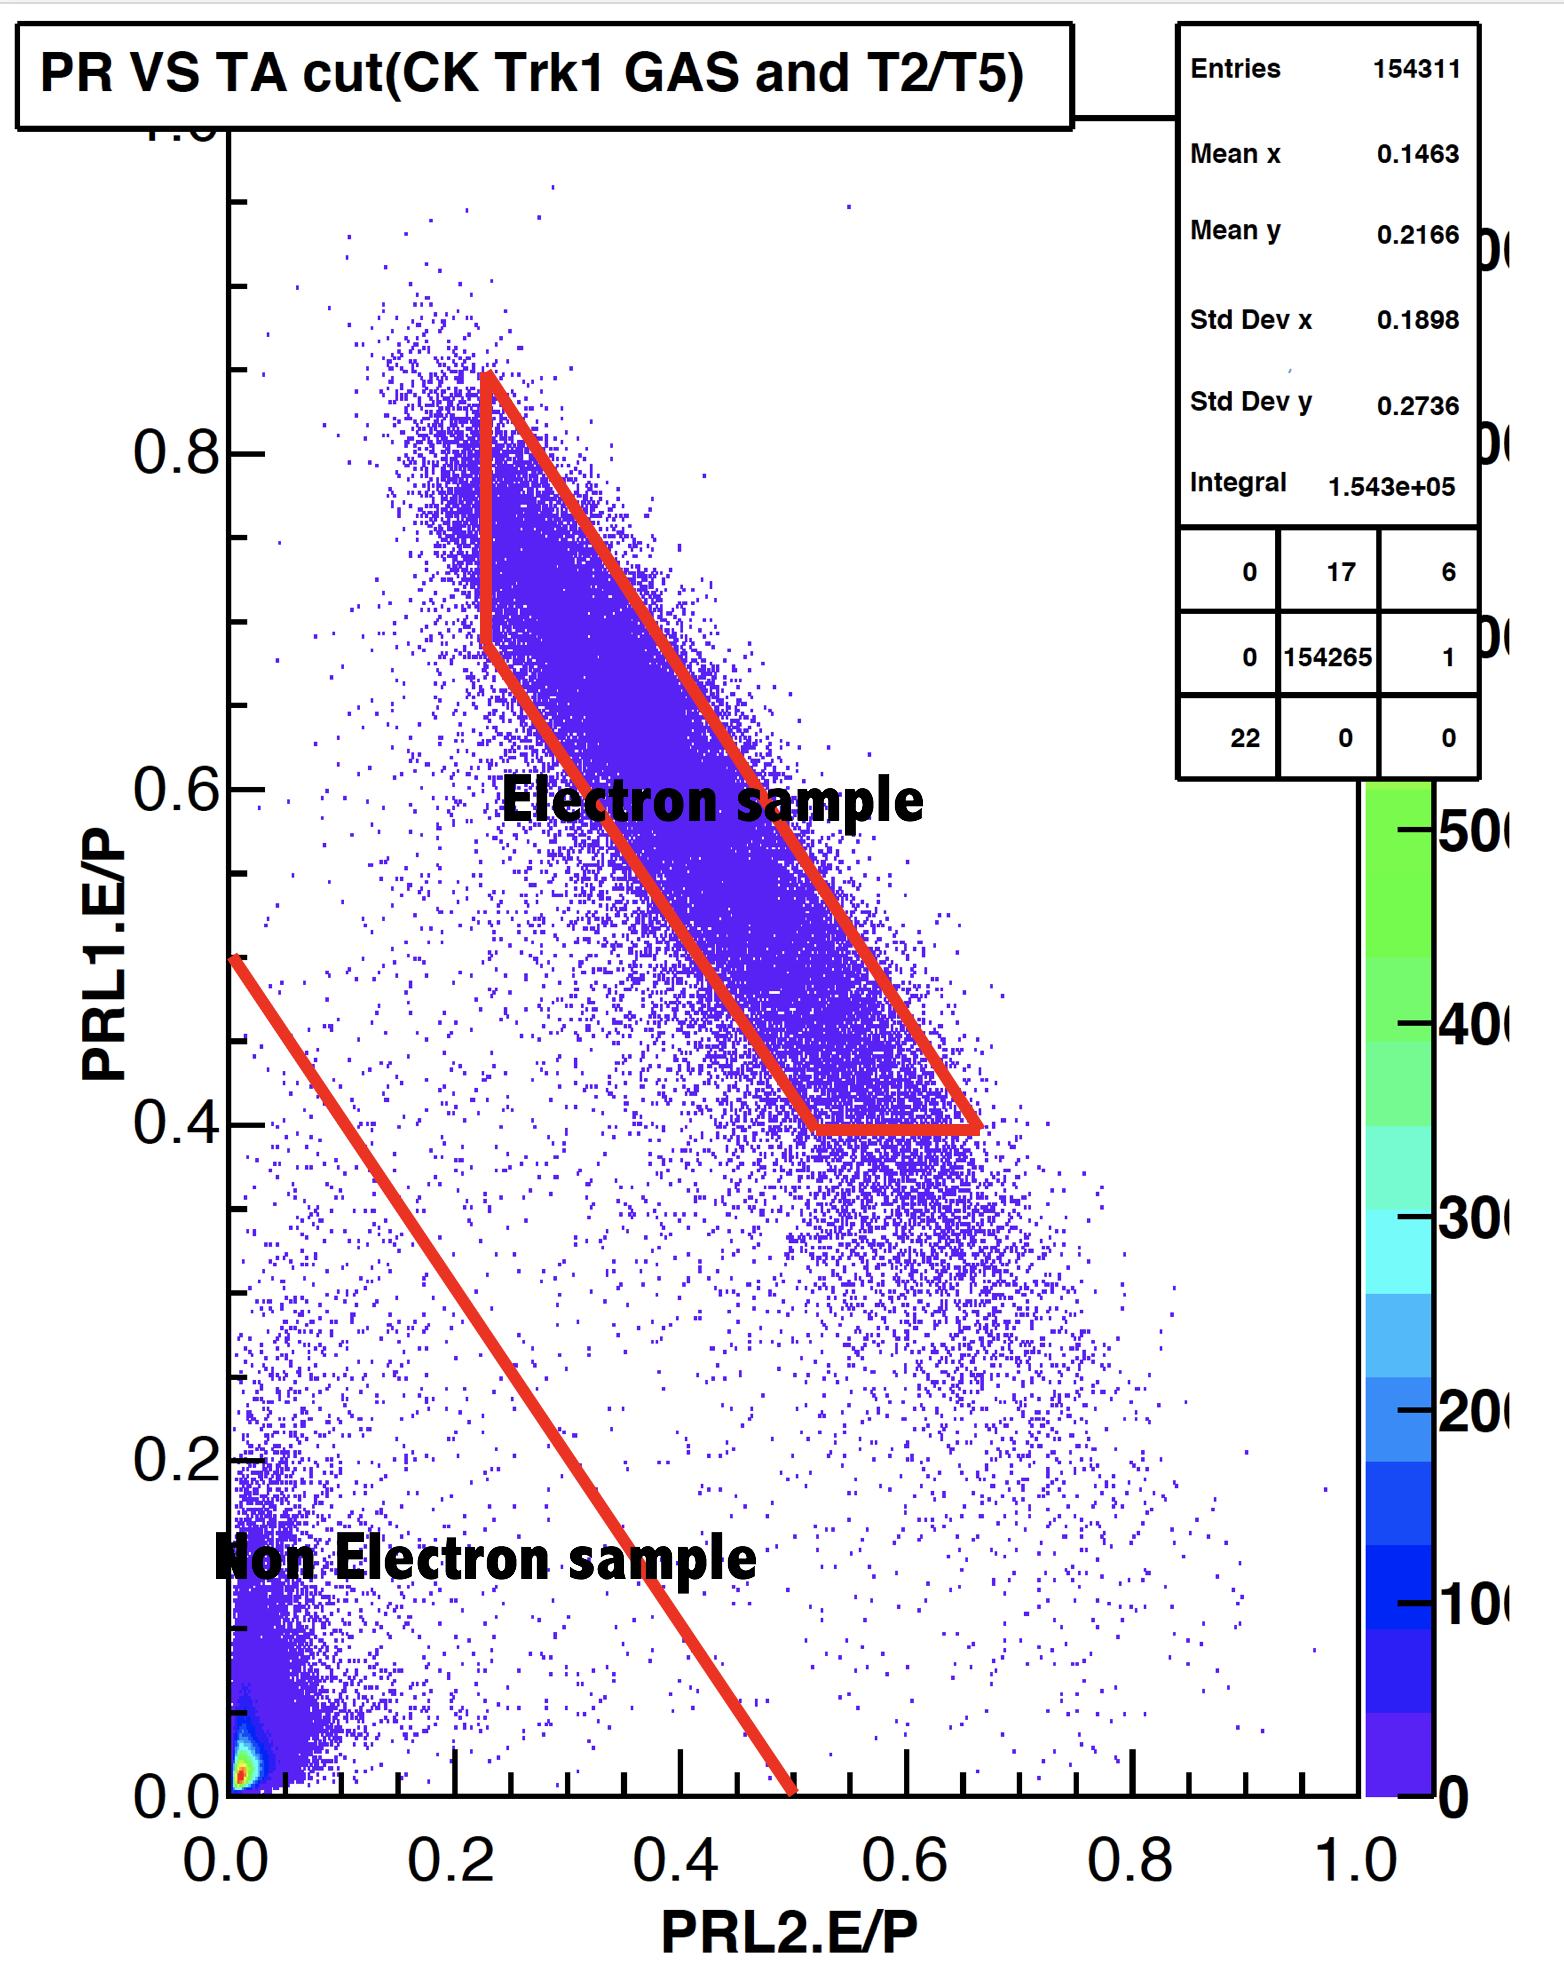
\includegraphics[width=0.4\textwidth] {./pid_plot/PID3.png}
 		\caption{electron and non-electron selecting from the calorimeter } \label{sample3}
 	\end{center}
\end{figure}   
 
 
then according the traditional way to check PID efficiency, the $P_{a}^{x}$ and $P_{a}^{e}$ can be calculable base on the Eq \ref{pid_eq1}. Since Cherenkov should behave stable for electron so the $P_{a}^{e}$ should be very close to 1 and its fluctuation should be very small by different kinematic settings. $P_{a}^{x}$ by contrast, is an effective efficiency for two different kinds signals which can be varied by different kinematic settings because of the different rations of X1 and X2 . Utilizing the independence of the two detectors and the following four functions

\begin{equation}  
\left\{  
             \begin{array}{lr}  
             N_{e}+N_{x}=N_{0} \\  
             P_{a}^{e} N_{e}+ P_{a}^{x} N_{x}=N_{1} \\    
             P_{b}^{e} N_{e}+ P_{b}^{x} N_{x}=N_{2} \\     
             P_{a}^{e} P_{b}^{e} N_{e}+ P_{a}^{x} P_{b}^{x} N_{x}=N_{3}\\  
             \end{array}  
\right.  
\label{PID_eq2}
\end{equation}  

The $P_{b}^{e}$,$P_{b}^{x}$,$N_{x}$,$N_{e}$ can be solved. Where the $N_{0}$ is the event number with the following general cut
\begin{equation}  \label{pid_eq3}
\left\{  
             \begin{array}{lr}  
             No \quad of \quad Track ==1 \\  
             -60\quad mrad< \theta_{tg} <60 \quad mrad \\    
             -30\quad mrad<\varphi_{tg} <30\quad  mrad  \\     
             -0.04<dp<0.04\\
             \beta>0  \\
             T2 \quad trigger\quad only
             \end{array}  
\right.  
\end{equation}  
$N_{1}(N_{2})$is the event number with just  additional Cherenkov (E/P) cut  and $N_{3}$ is the event number with two pid detector cut. $N_{x}(N_{e}) $ is the number of non-electrons(electrons) totally in our data after the previous cut. 

The following four plots(Fig \ref{PPID3} and Fig \ref{PPID4}) shows the four efficiencies defined previous for the two PID detectors, and as we can see three of them ($P_{b}^{e}$,$P_{b}^{x}$,$P_{a}^{e}$) are behaved stable for different kinematics and the $P_{a}^{x}$ varies as what we expected.
\begin{figure}[htpb]

\subfigure[electron effciency for Cherenkov]{
\begin{minipage}[t]{1\linewidth}

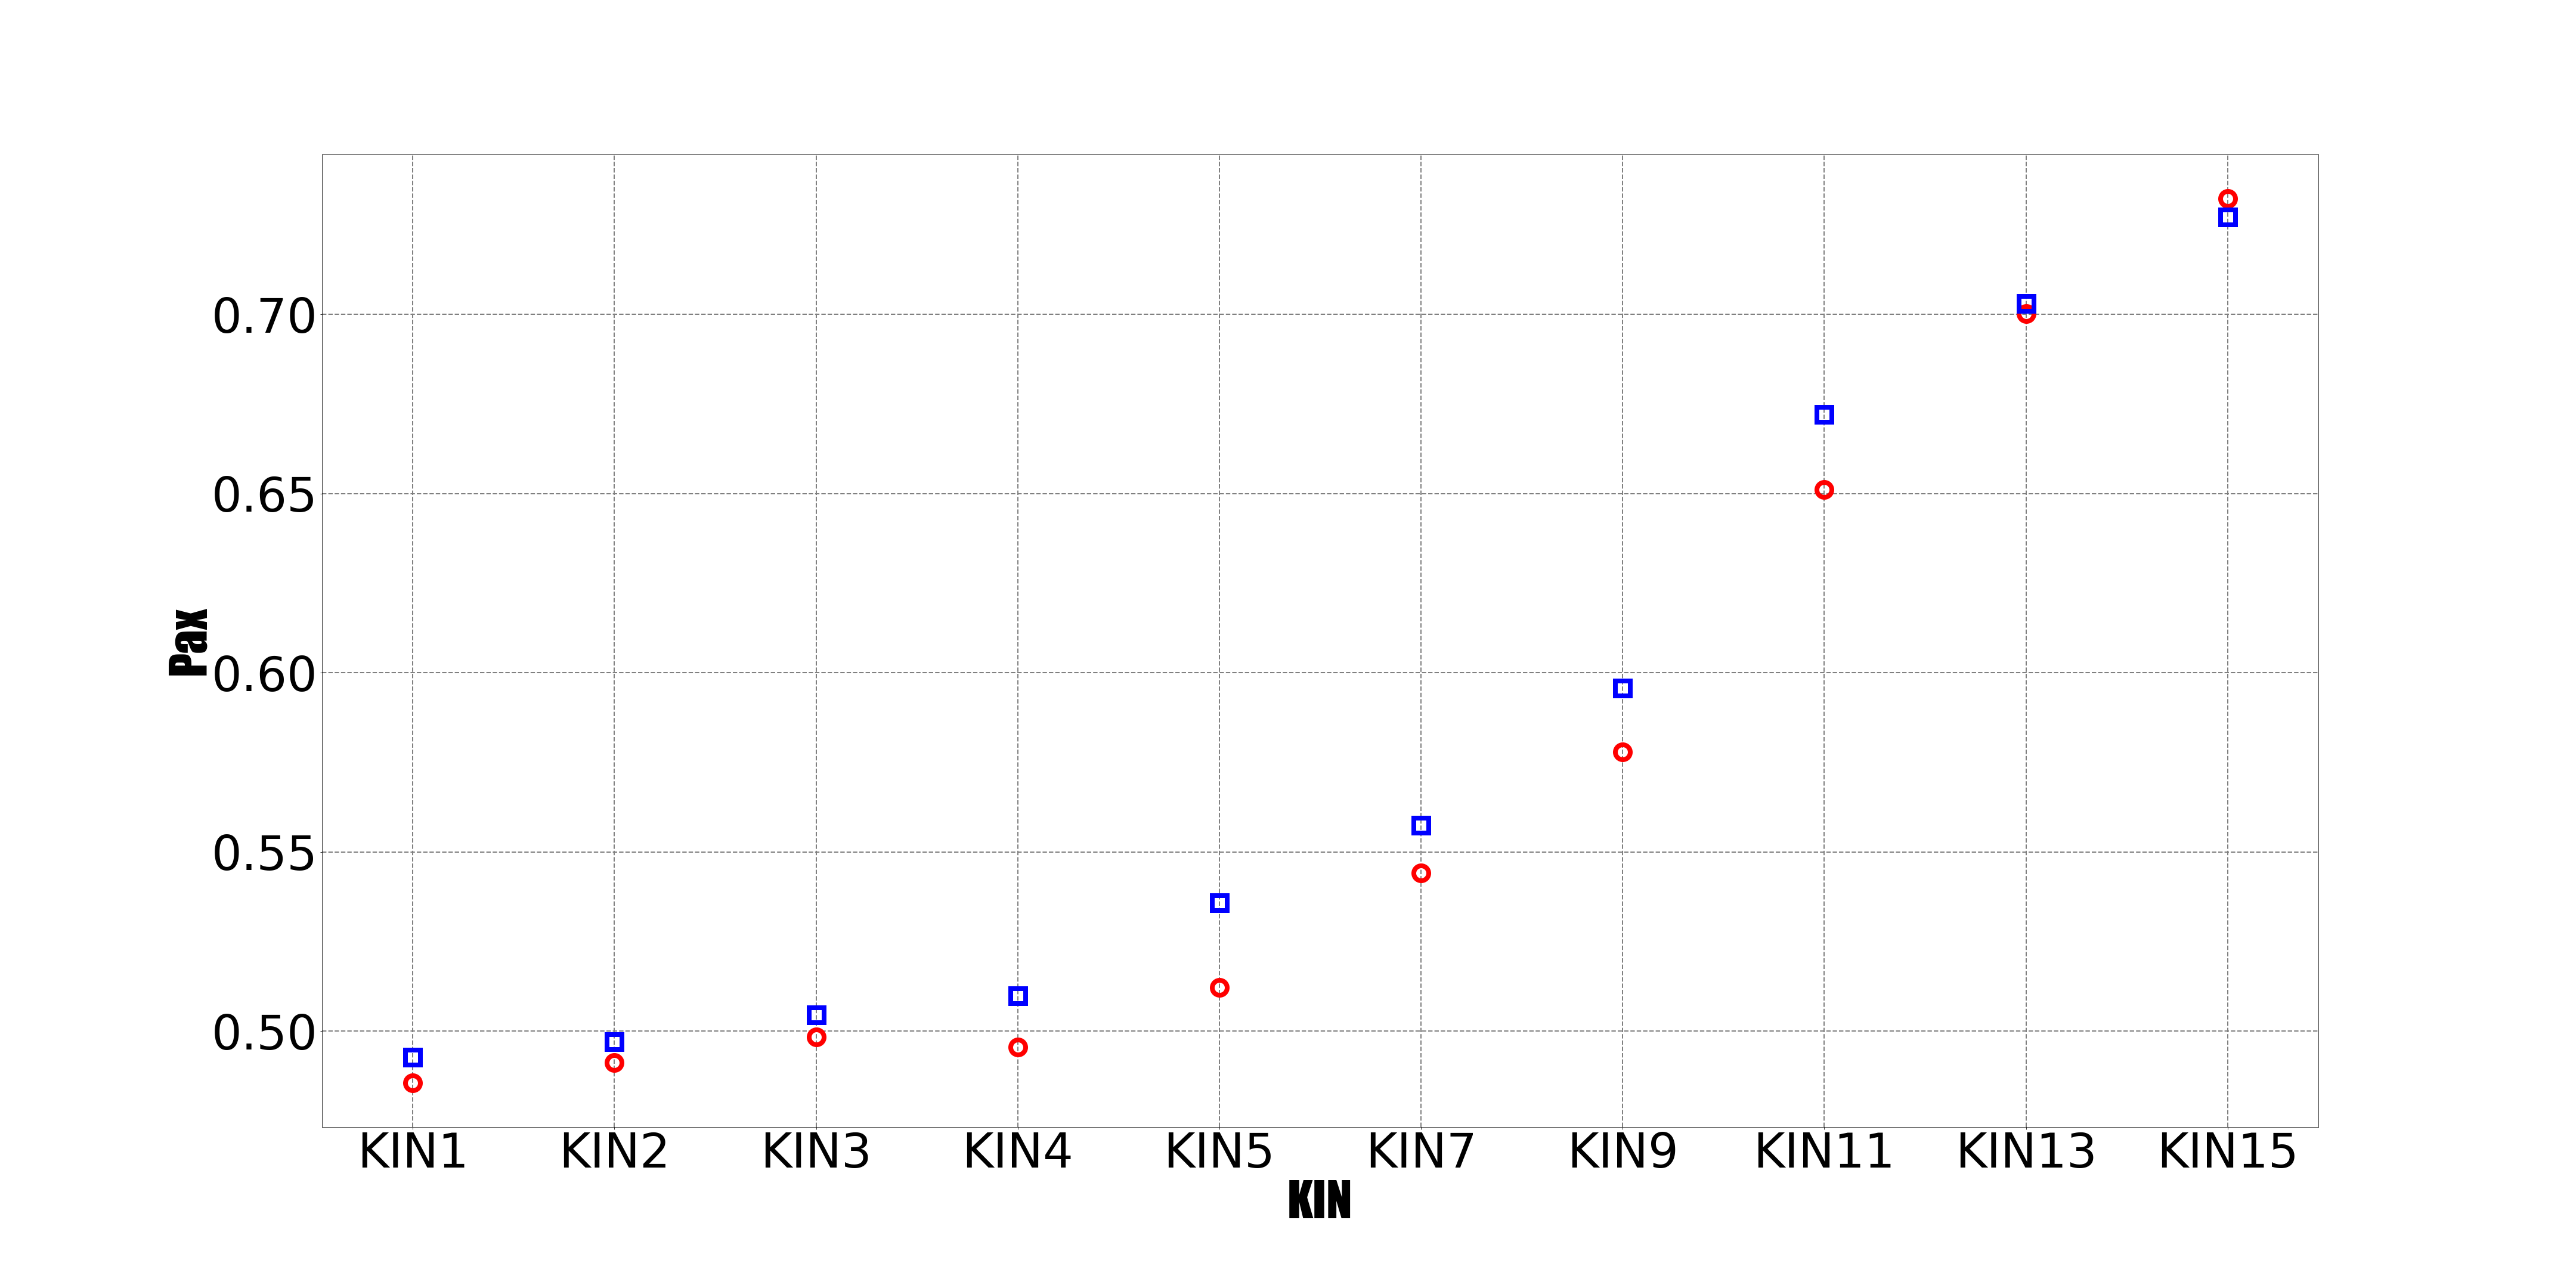
\includegraphics[width=3in]{./pid_plot/PIDD1.png}
\end{minipage}
}
\subfigure[non-electron effciency for Cherenkov]{
\begin{minipage}[t]{1\linewidth}

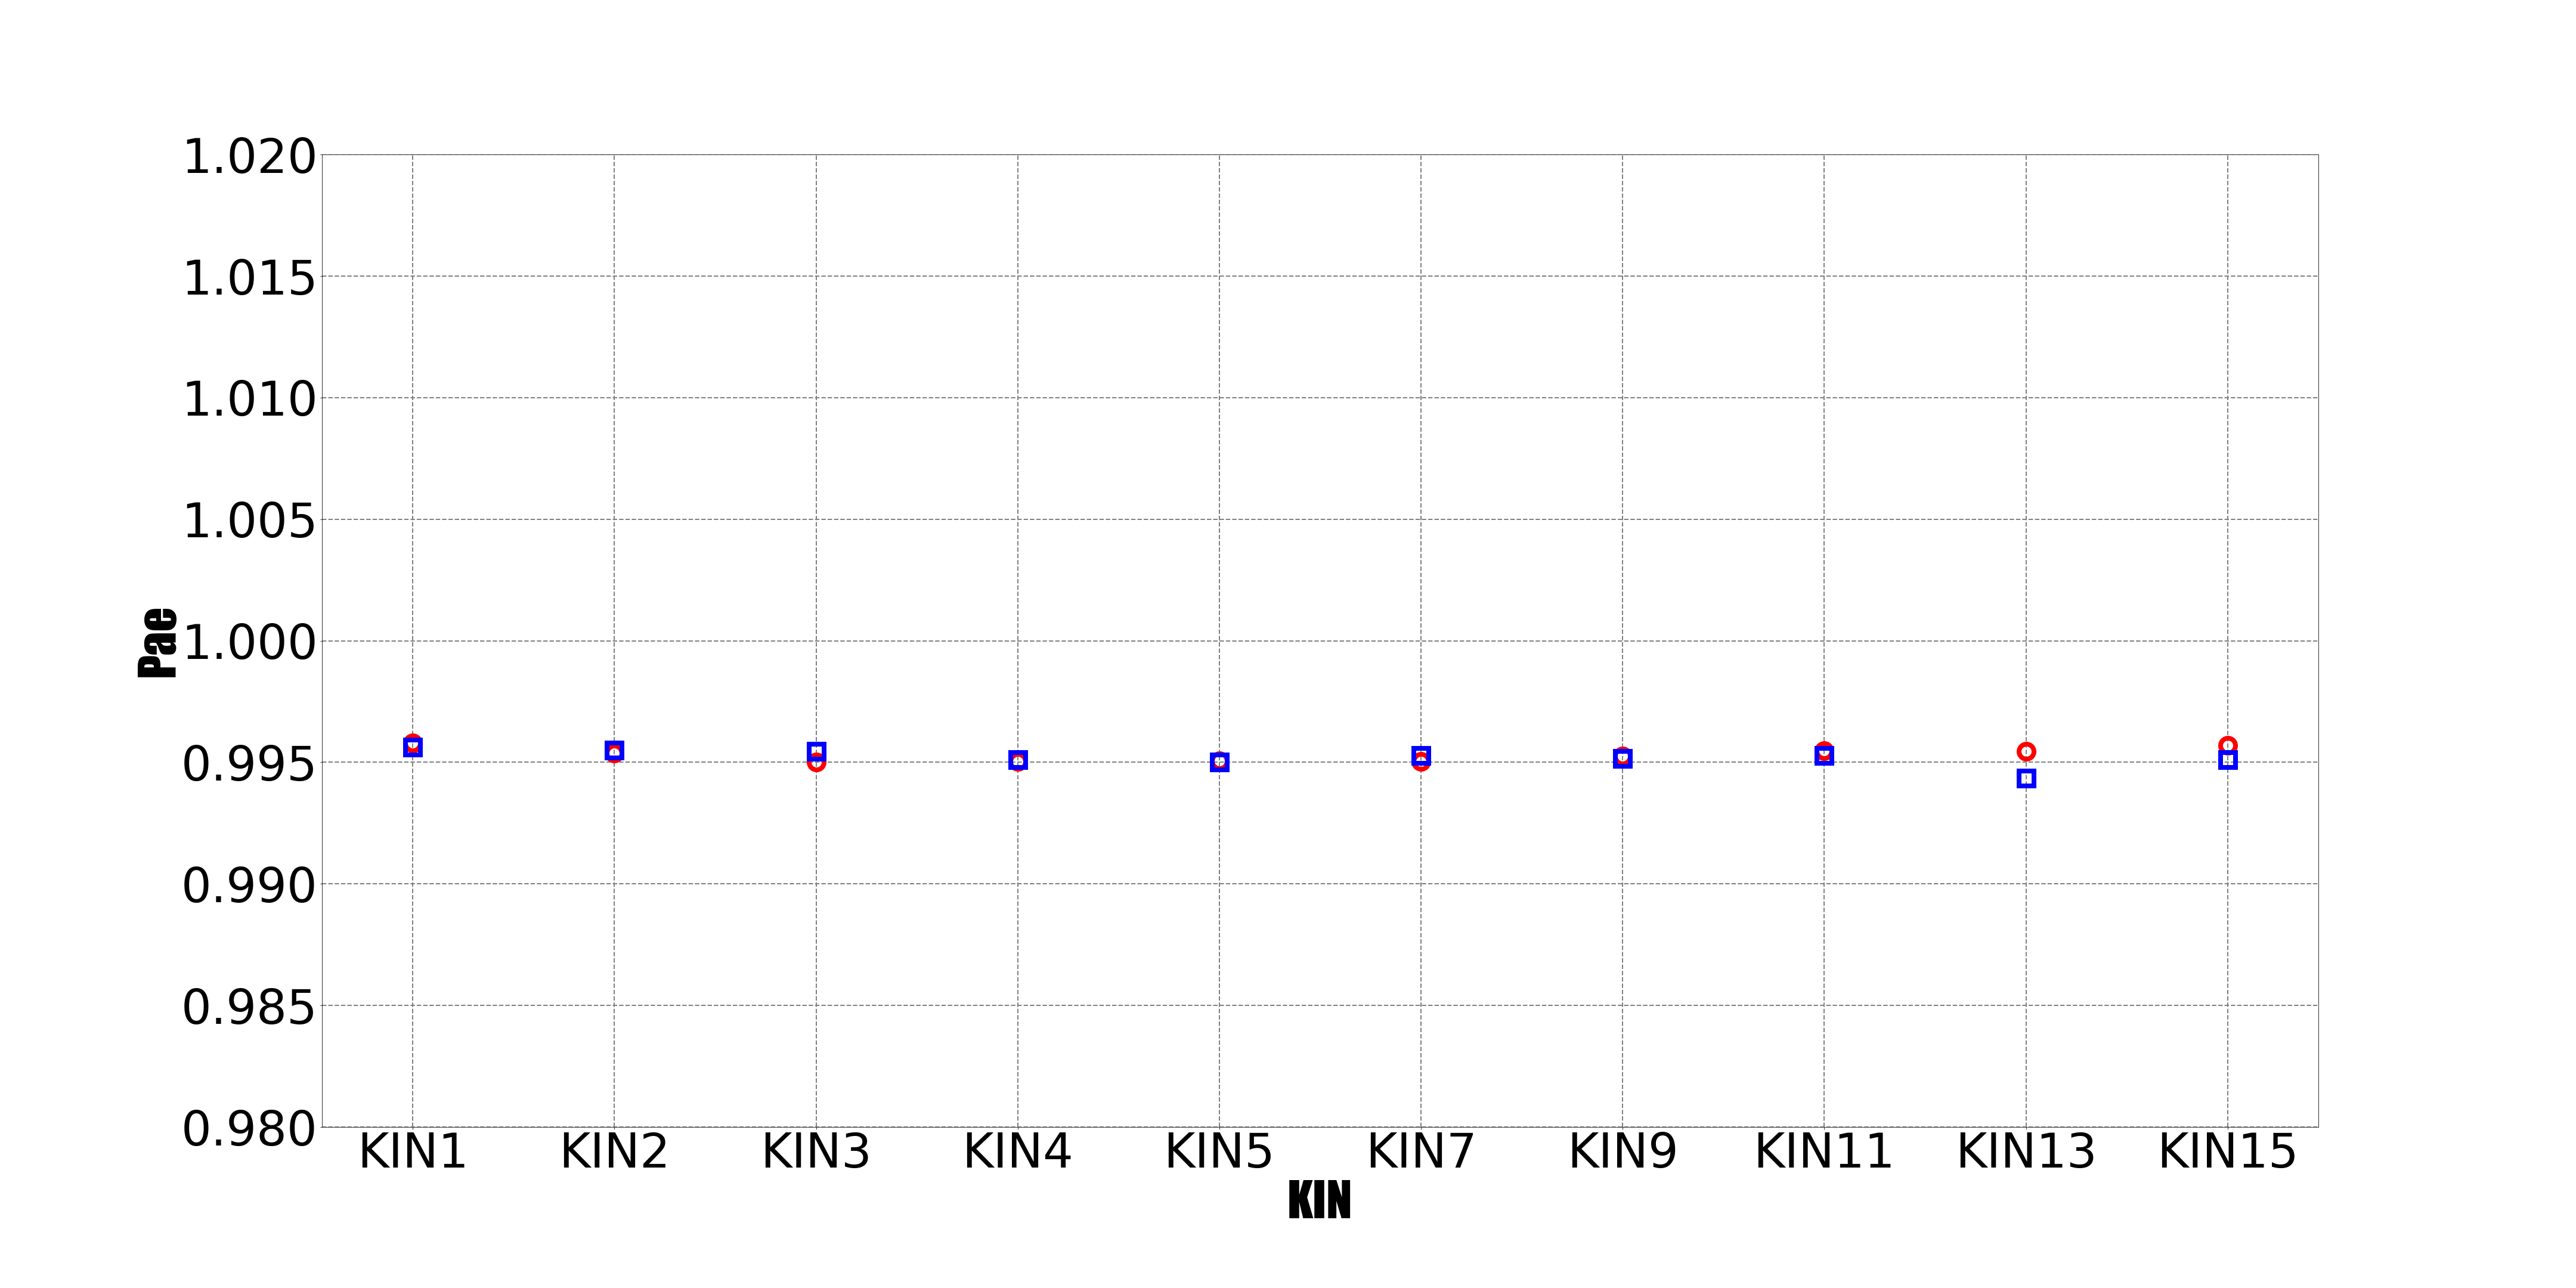
\includegraphics[width=3in]{./pid_plot/PIDD2.png}
\end{minipage}
}

\caption{The two PID efficiency for Chenerkov with different kinematic settings (Blue: He3 and Red: H3)  }  \label{PPID3}
\end{figure}

\begin{figure}[htpb] 
\subfigure[electron effciency for calorimeter ]{
\begin{minipage}[t]{1\linewidth}

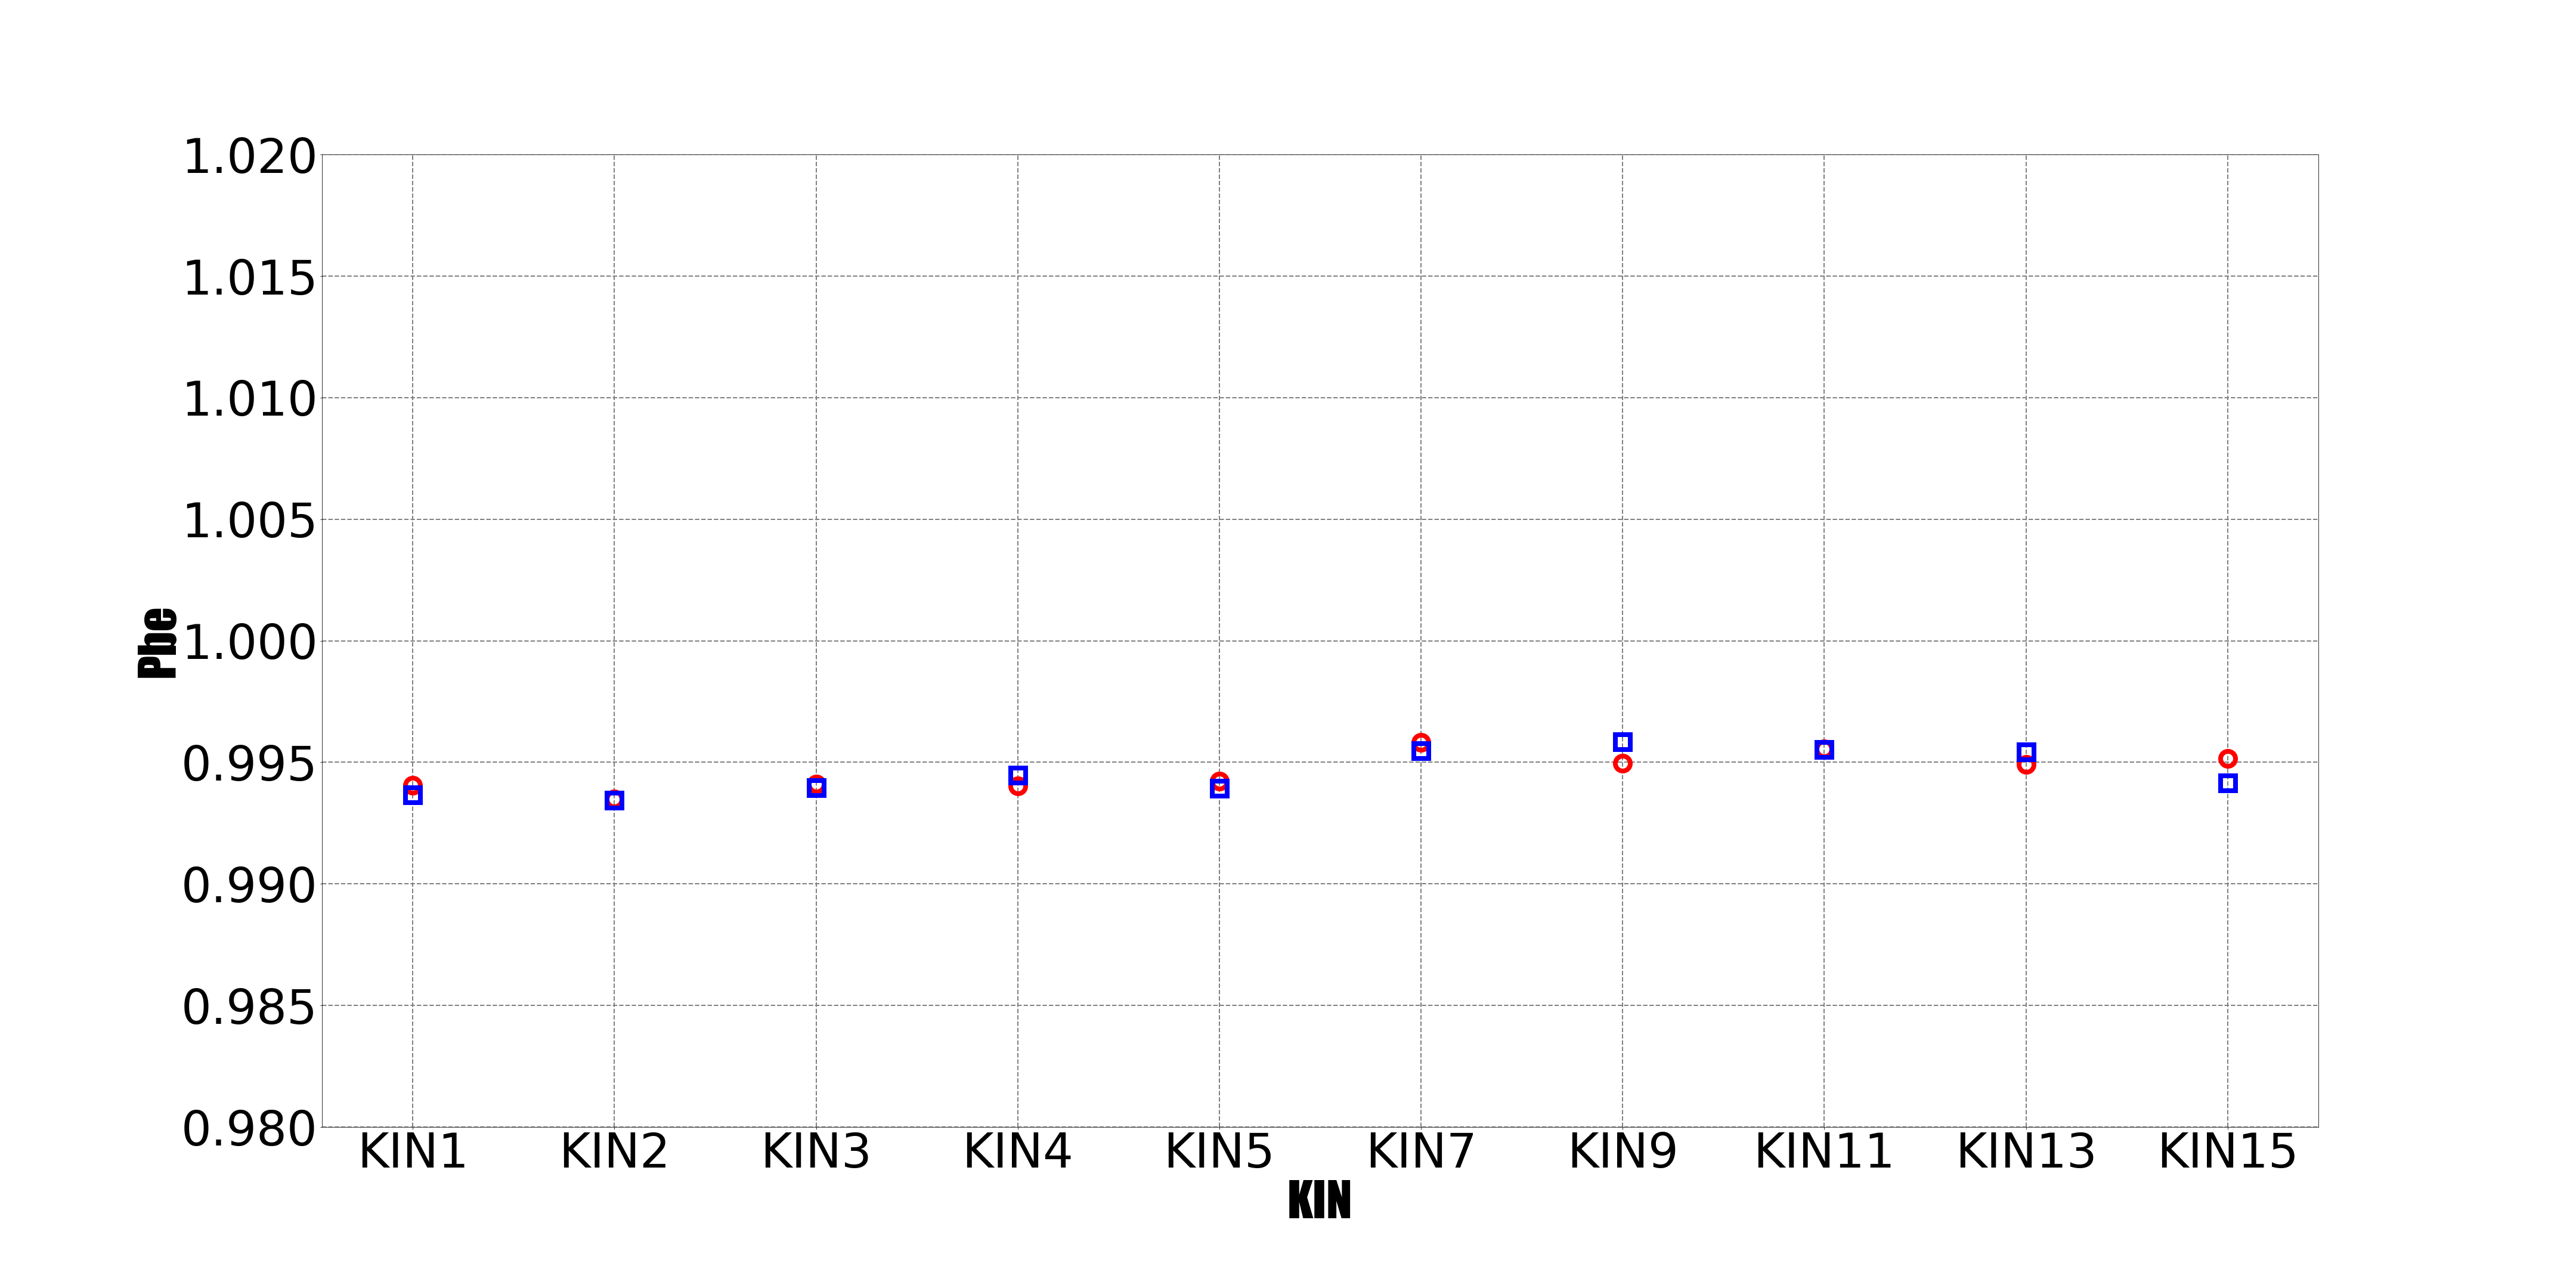
\includegraphics[width=3in]{./pid_plot/PIDD3.png}
\end{minipage}
}
\subfigure[electron effciency for calorimeter]{
\begin{minipage}[t]{1\linewidth}

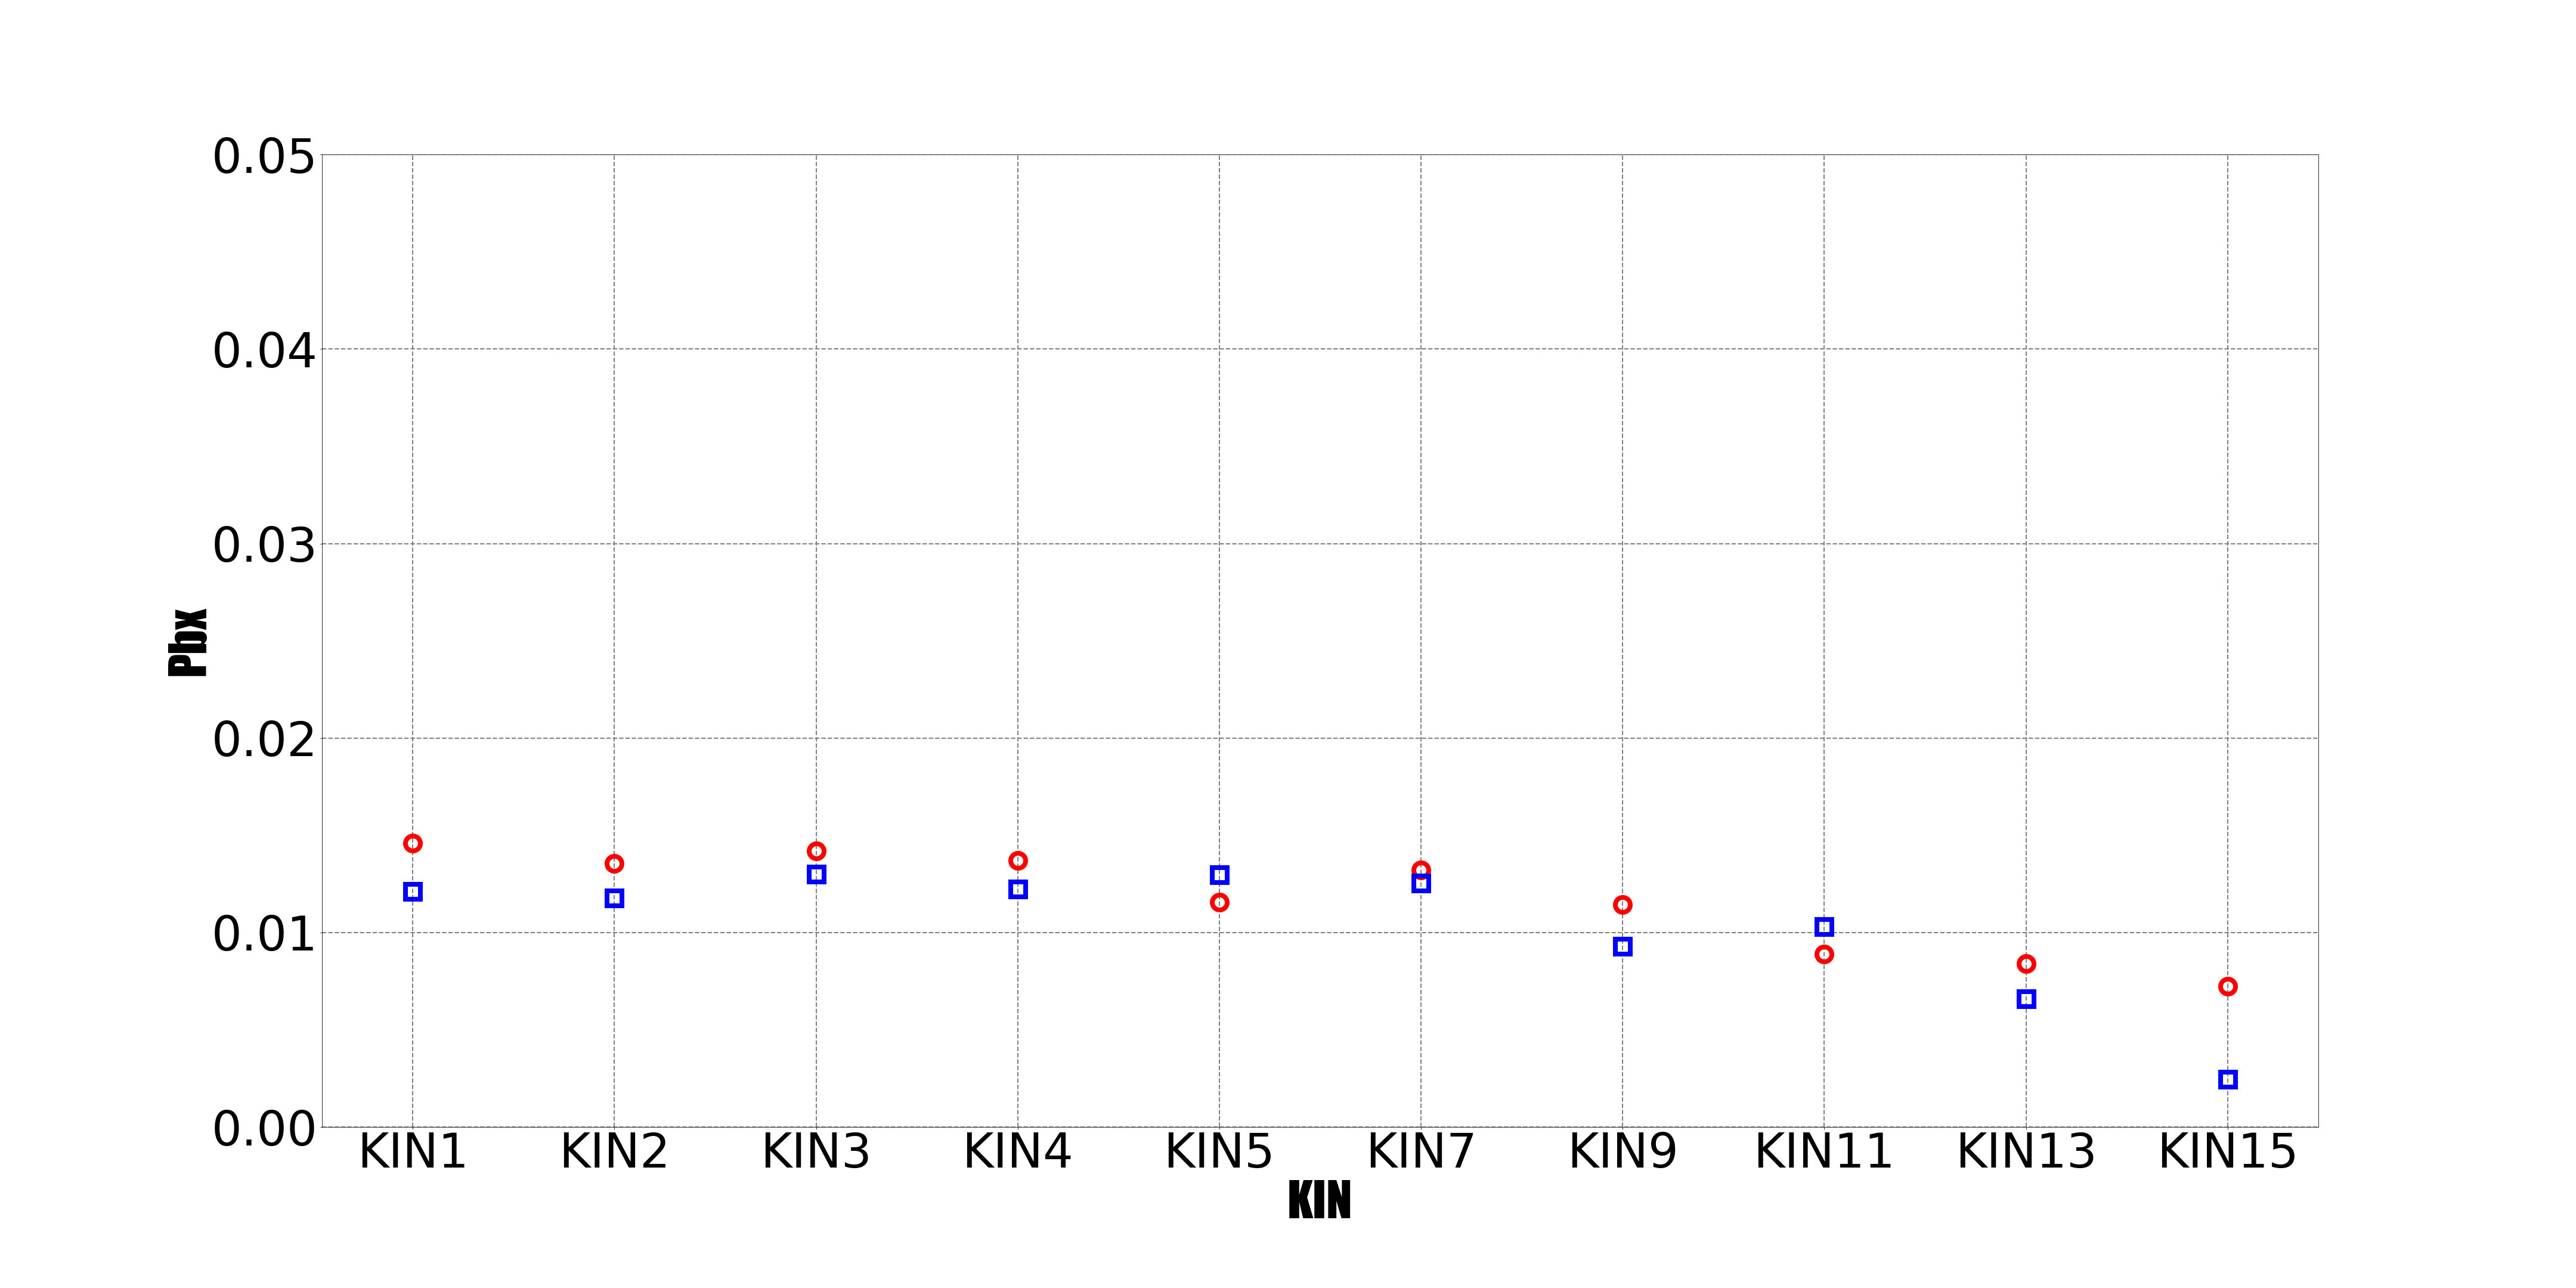
\includegraphics[width=3in]{./pid_plot/PID4.png}
\end{minipage}
}

\caption{The two PID efficiency for calorimeter with different kinematic settings  (Blue: He3 and Red: H3)  } \label{PPID4}
\end{figure}



 Since we only analysis electrons, for a certain PID cuts, we cares more about the non-electron contamination. Define 
\begin{equation}  
\left\{   \begin{array}{lr} 
             N_{e}^{TRUE}= P_{a}^{e} P_{b}^{e} N_{e}\\
             N_{e}^{FALSE}= P_{a}^{x} P_{b}^{x} N_{x}
             \end{array}  
\right.  
\end{equation}  
Where the $N_{e}^{FALSE}$ is the non-electron can pass our two PID cuts and $N_{e}^{TRUE}$ is the number of electrons can pass the same cuts, then the non-electron contamination can be calculated by the following 
\begin{equation}\label{eq:eff1}
\dfrac{x}{e}=\dfrac{N_{e}^{FALSE}}{N_{e}^{TRUE}+N_{e}^{FALSE}}
\end{equation}
Fig \ref{PPID5} shows the non-electron contamination at different kinematics settings, as we can see, this contamination is at 10-3 to 10-4 level (even smaller if only cross-section ratio be focused).                                                               
 
\begin{figure}
 	
 		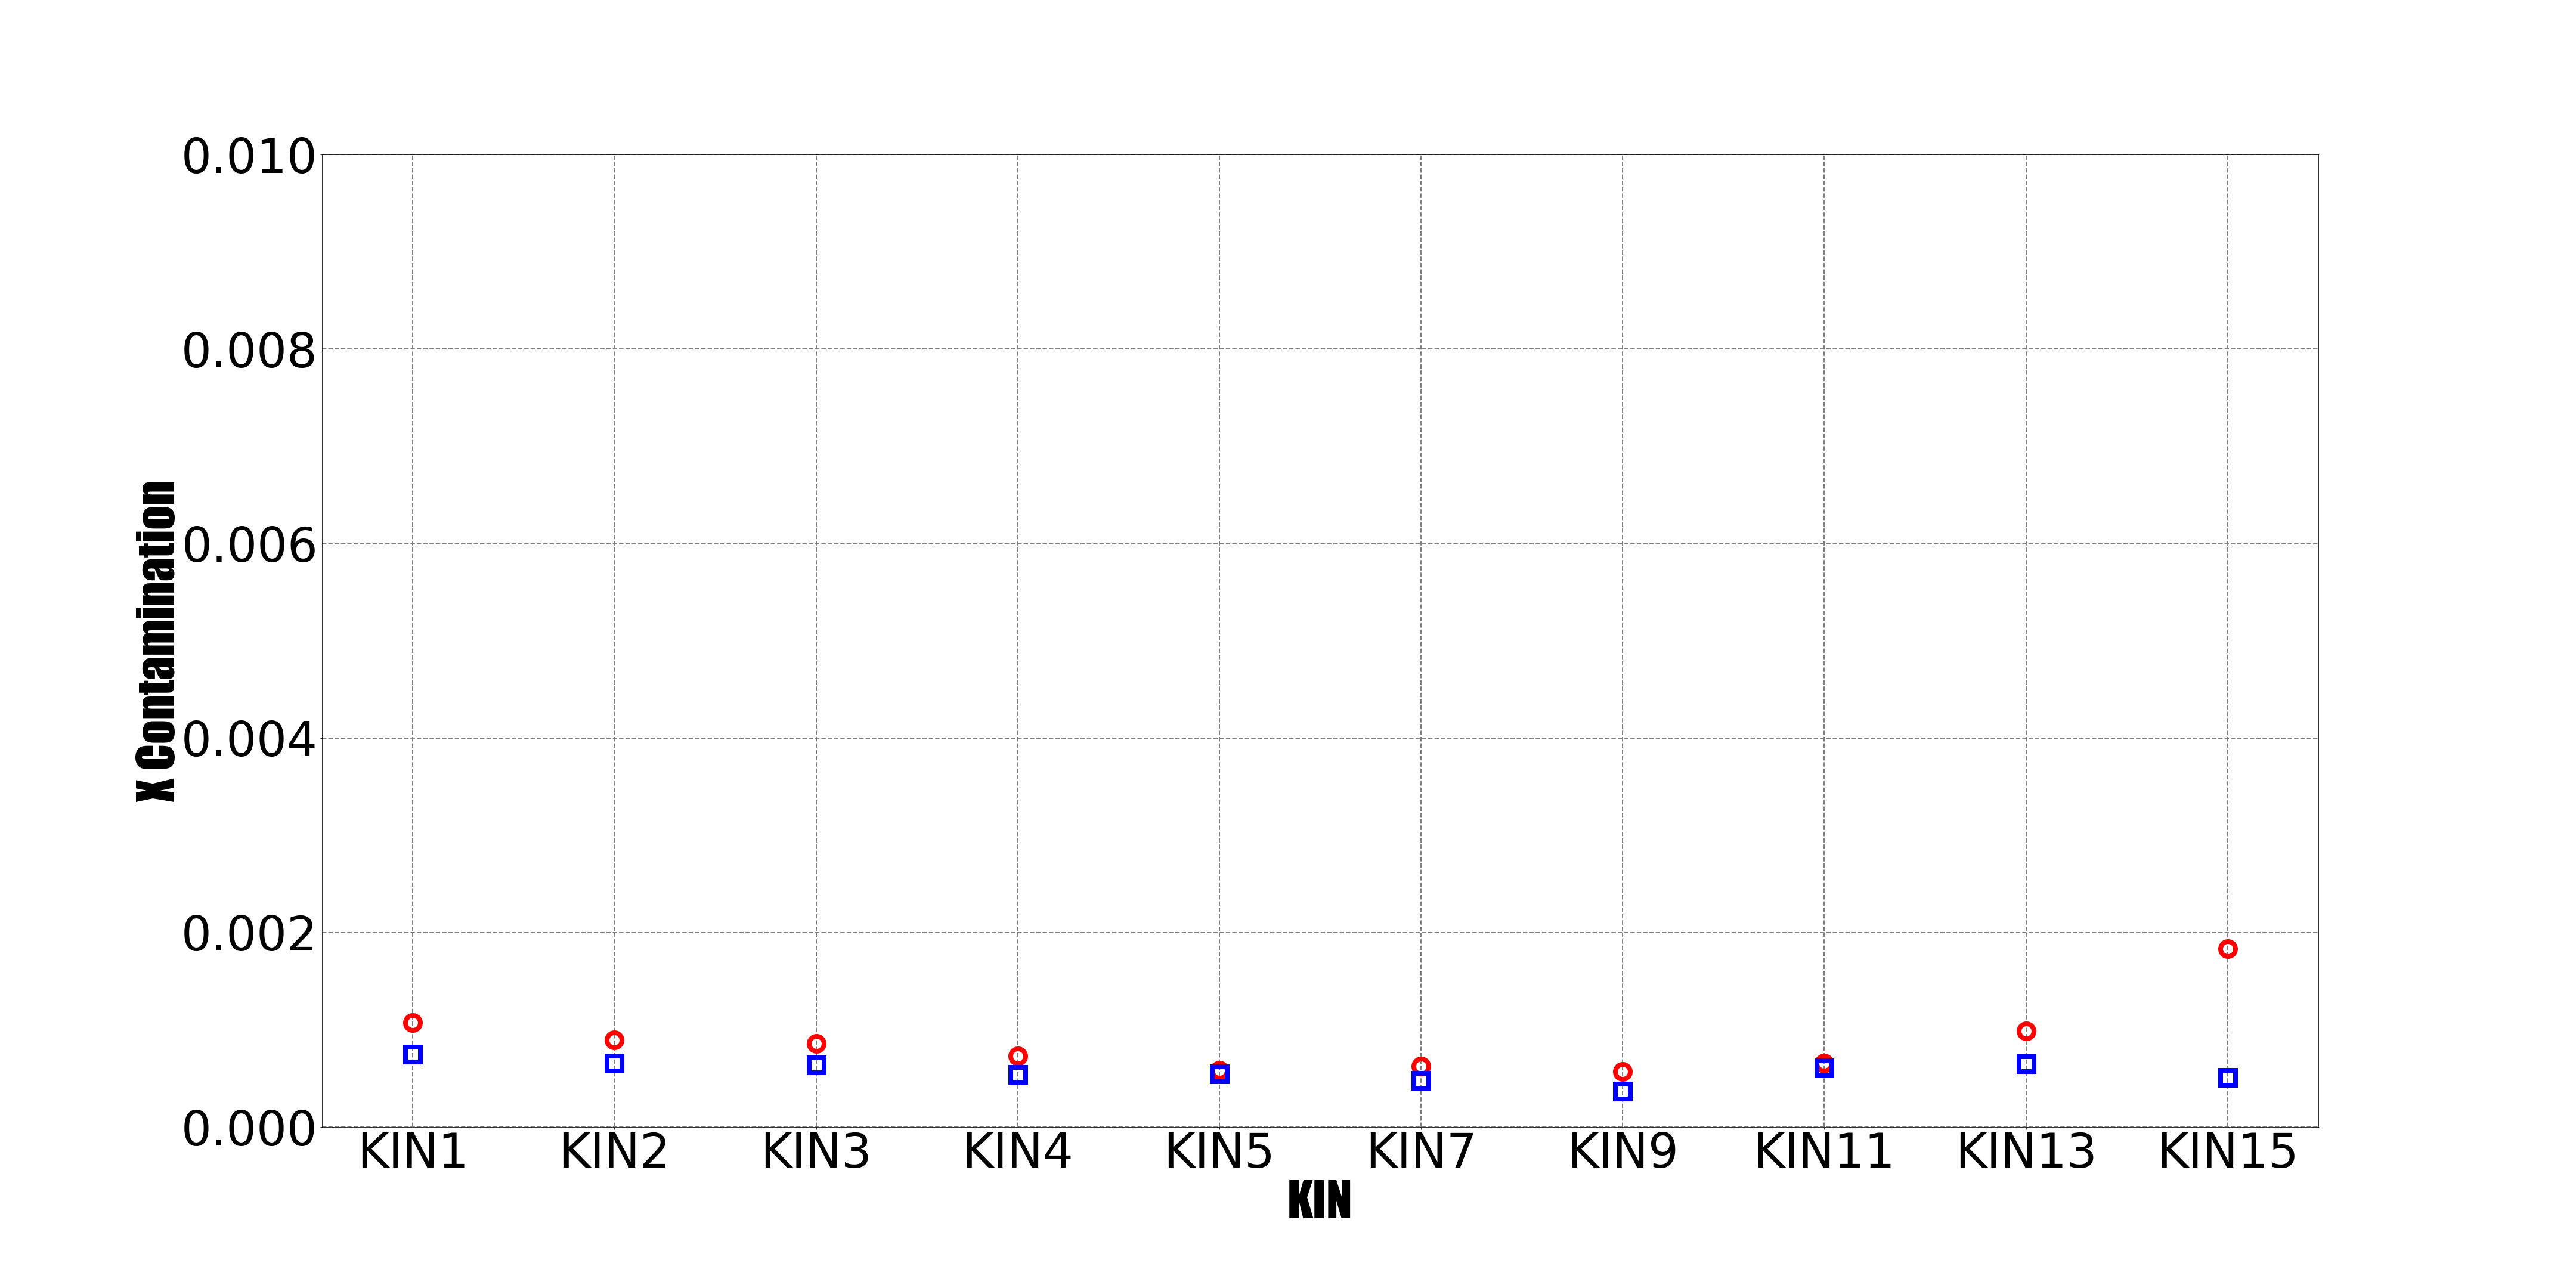
\includegraphics[width=0.5\textwidth]{./pid_plot/PID5.png}
 		\caption{ Non-electron contimination for H3(Red) and He3(Blue) with different kinematic setting  } \label{PPID5}
 	
\end{figure}   
 
%\bibliographystyle{plain}
%\bibliography{ref}




 \subsection{i. Positron Subtraction}
  (Tong Su)
%opening
The high energy photons radiated from electrons in the target can decay into electron-positron pairs. These electrons can also be detected by the spectrometers and we cannot distinguish them from the scattering electrons just base on their performance in the detectors. To determine the magnitude of this background and eliminate them from our data, we can use the charge-symmetric features of this background and just measure the positrons yields to meet our goals with the following relations
\begin{equation}\label{postiron_eq1}
\dfrac{Y_{e-}^{BK}}{Y_{e-}^{tot}}=\dfrac{Y_{e-}^{BK}}{Y_{e-}^{BK}+Y_{e-}^{DIS}}=\dfrac{Y_{e+}^{BK}}{Y_{e+}^{BK}+Y_{e-}^{DIS}}
\end{equation}  
Where the $Y_{e-}^{DIS}$ is the electron yield from deep inelastic scattering and $Y_{e+}^{BK}$ /$Y_{e-}^{DIS}$ is the positron(electron) yield from background

For MARATHON, positron measurements is performed at KIN1, KIN3, KIN5 for H3 , D2,He3 as well as empty cell and KIN1 ,KIN3 for H1. And Yields for the positron data is 
\begin{equation}\label{postiron_eq2}
Y_{e+}^{BK}=\dfrac{N_{e+}}{C*LT*\rho} \times Correction
\end{equation} 
Where $N_{e+}$ is the number of prositron, $LT$ is dead time correction ,C is the charge and $\rho$ is the density of the target.for positron analysis, the correcrtion include the endcap contimanation and non-positron contimation correction. Enpcap contimanation is similar with the electron analysis(See SectionXXX). To eliminate the non-positron background contimation, a combined exponential function for the background and a gauss peak function for the postion signal are used to fit the calorimeter E/P spectrum, the integration of the background tail beyond the E/P cut can be tread as the non-positron background(Fig \ref{po_1}).
\begin{figure}
 	\begin{center}
 		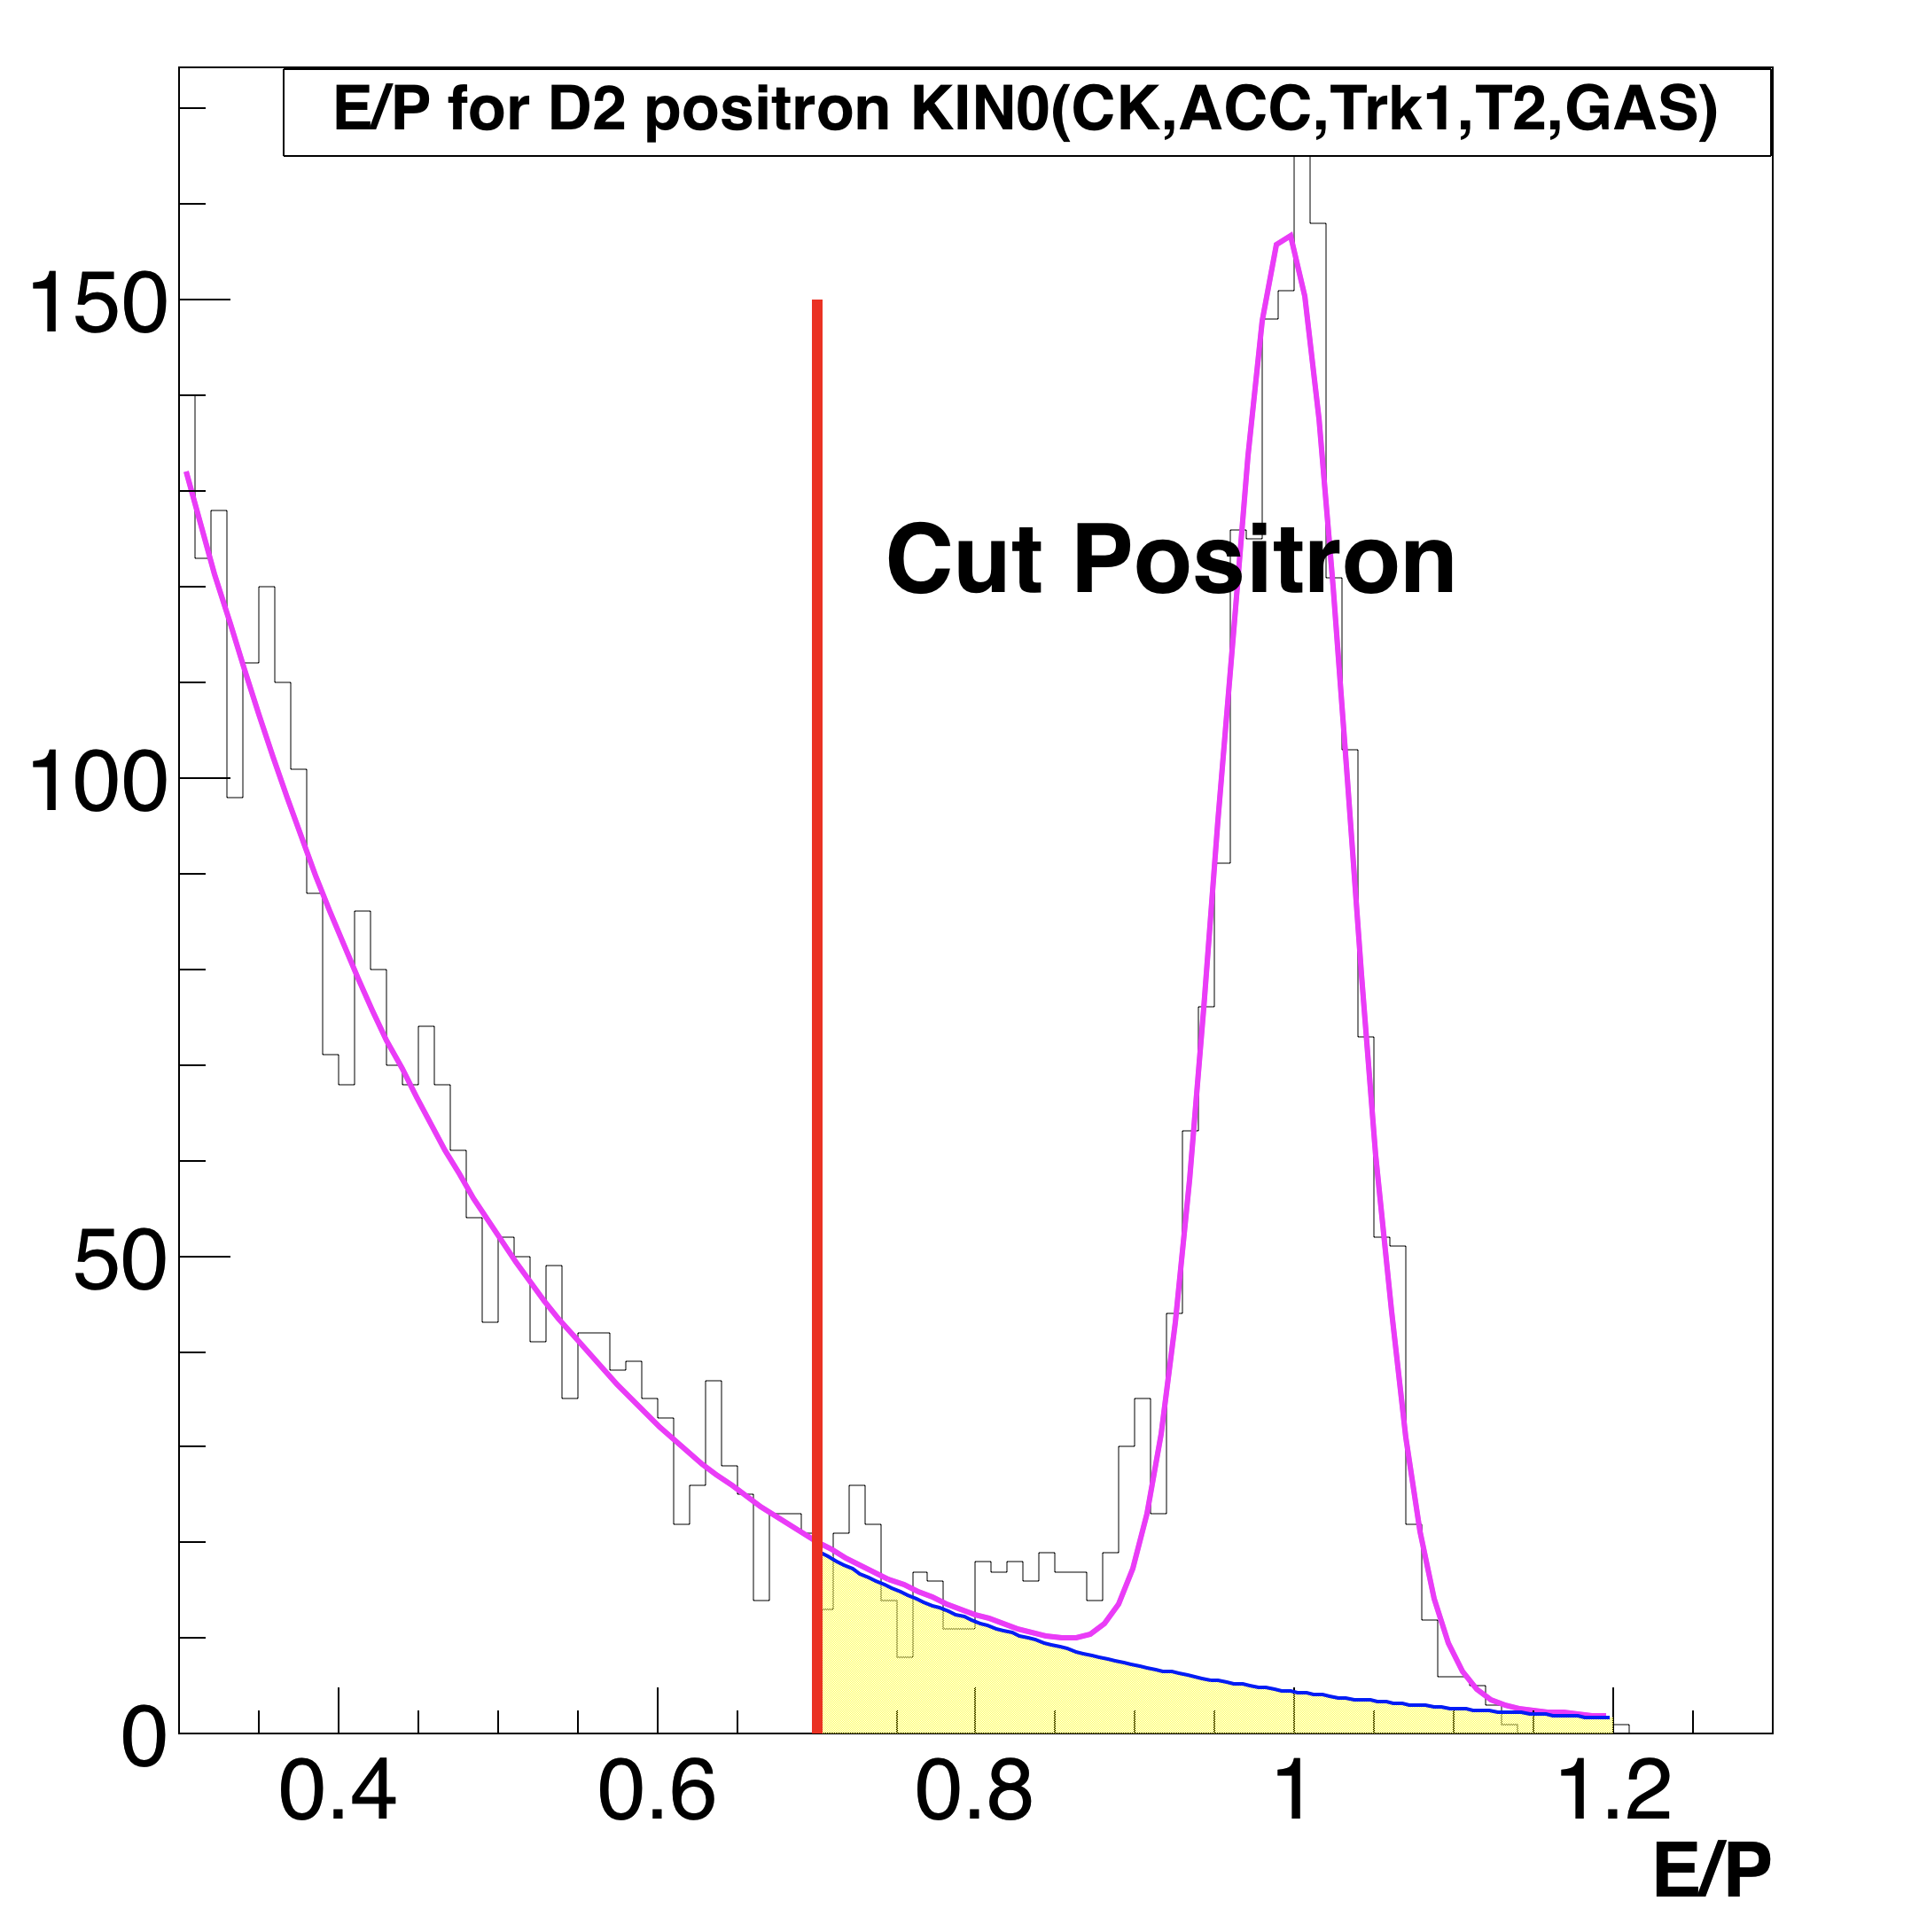
\includegraphics[width=0.4\textwidth] {./Positron_plot/Positron_1.png}
 		\caption{ The E/P spectrum for the KIN1 positron data , and the integration area of the expoential function( yellow shadow part) is the non-positron cotimatination} \label{po_1}
 	\end{center}
\end{figure}   

Combine with electrons with the corresponding kinematics settings, we can get the $Y_{e+}^{BK}/Y_{e-}^{tot}$, then a exponential function $f(x)=Ae_{-Bx}$ is performed to fit the $Y_{e+}^{BK}/Y_{e-}^{tot}$ . With this fitting function, charged-symmetric background be get rid of by 
\begin{equation}\label{postiron_eq1}
Y_{e-}^{DIS}=Y_{e-}^{tot}*\left(1-\dfrac{Y_{e+}^{BK}}{Y_{e-}^{tot}}\right)
\end{equation}  
\begin{figure}
 	\begin{center}
 		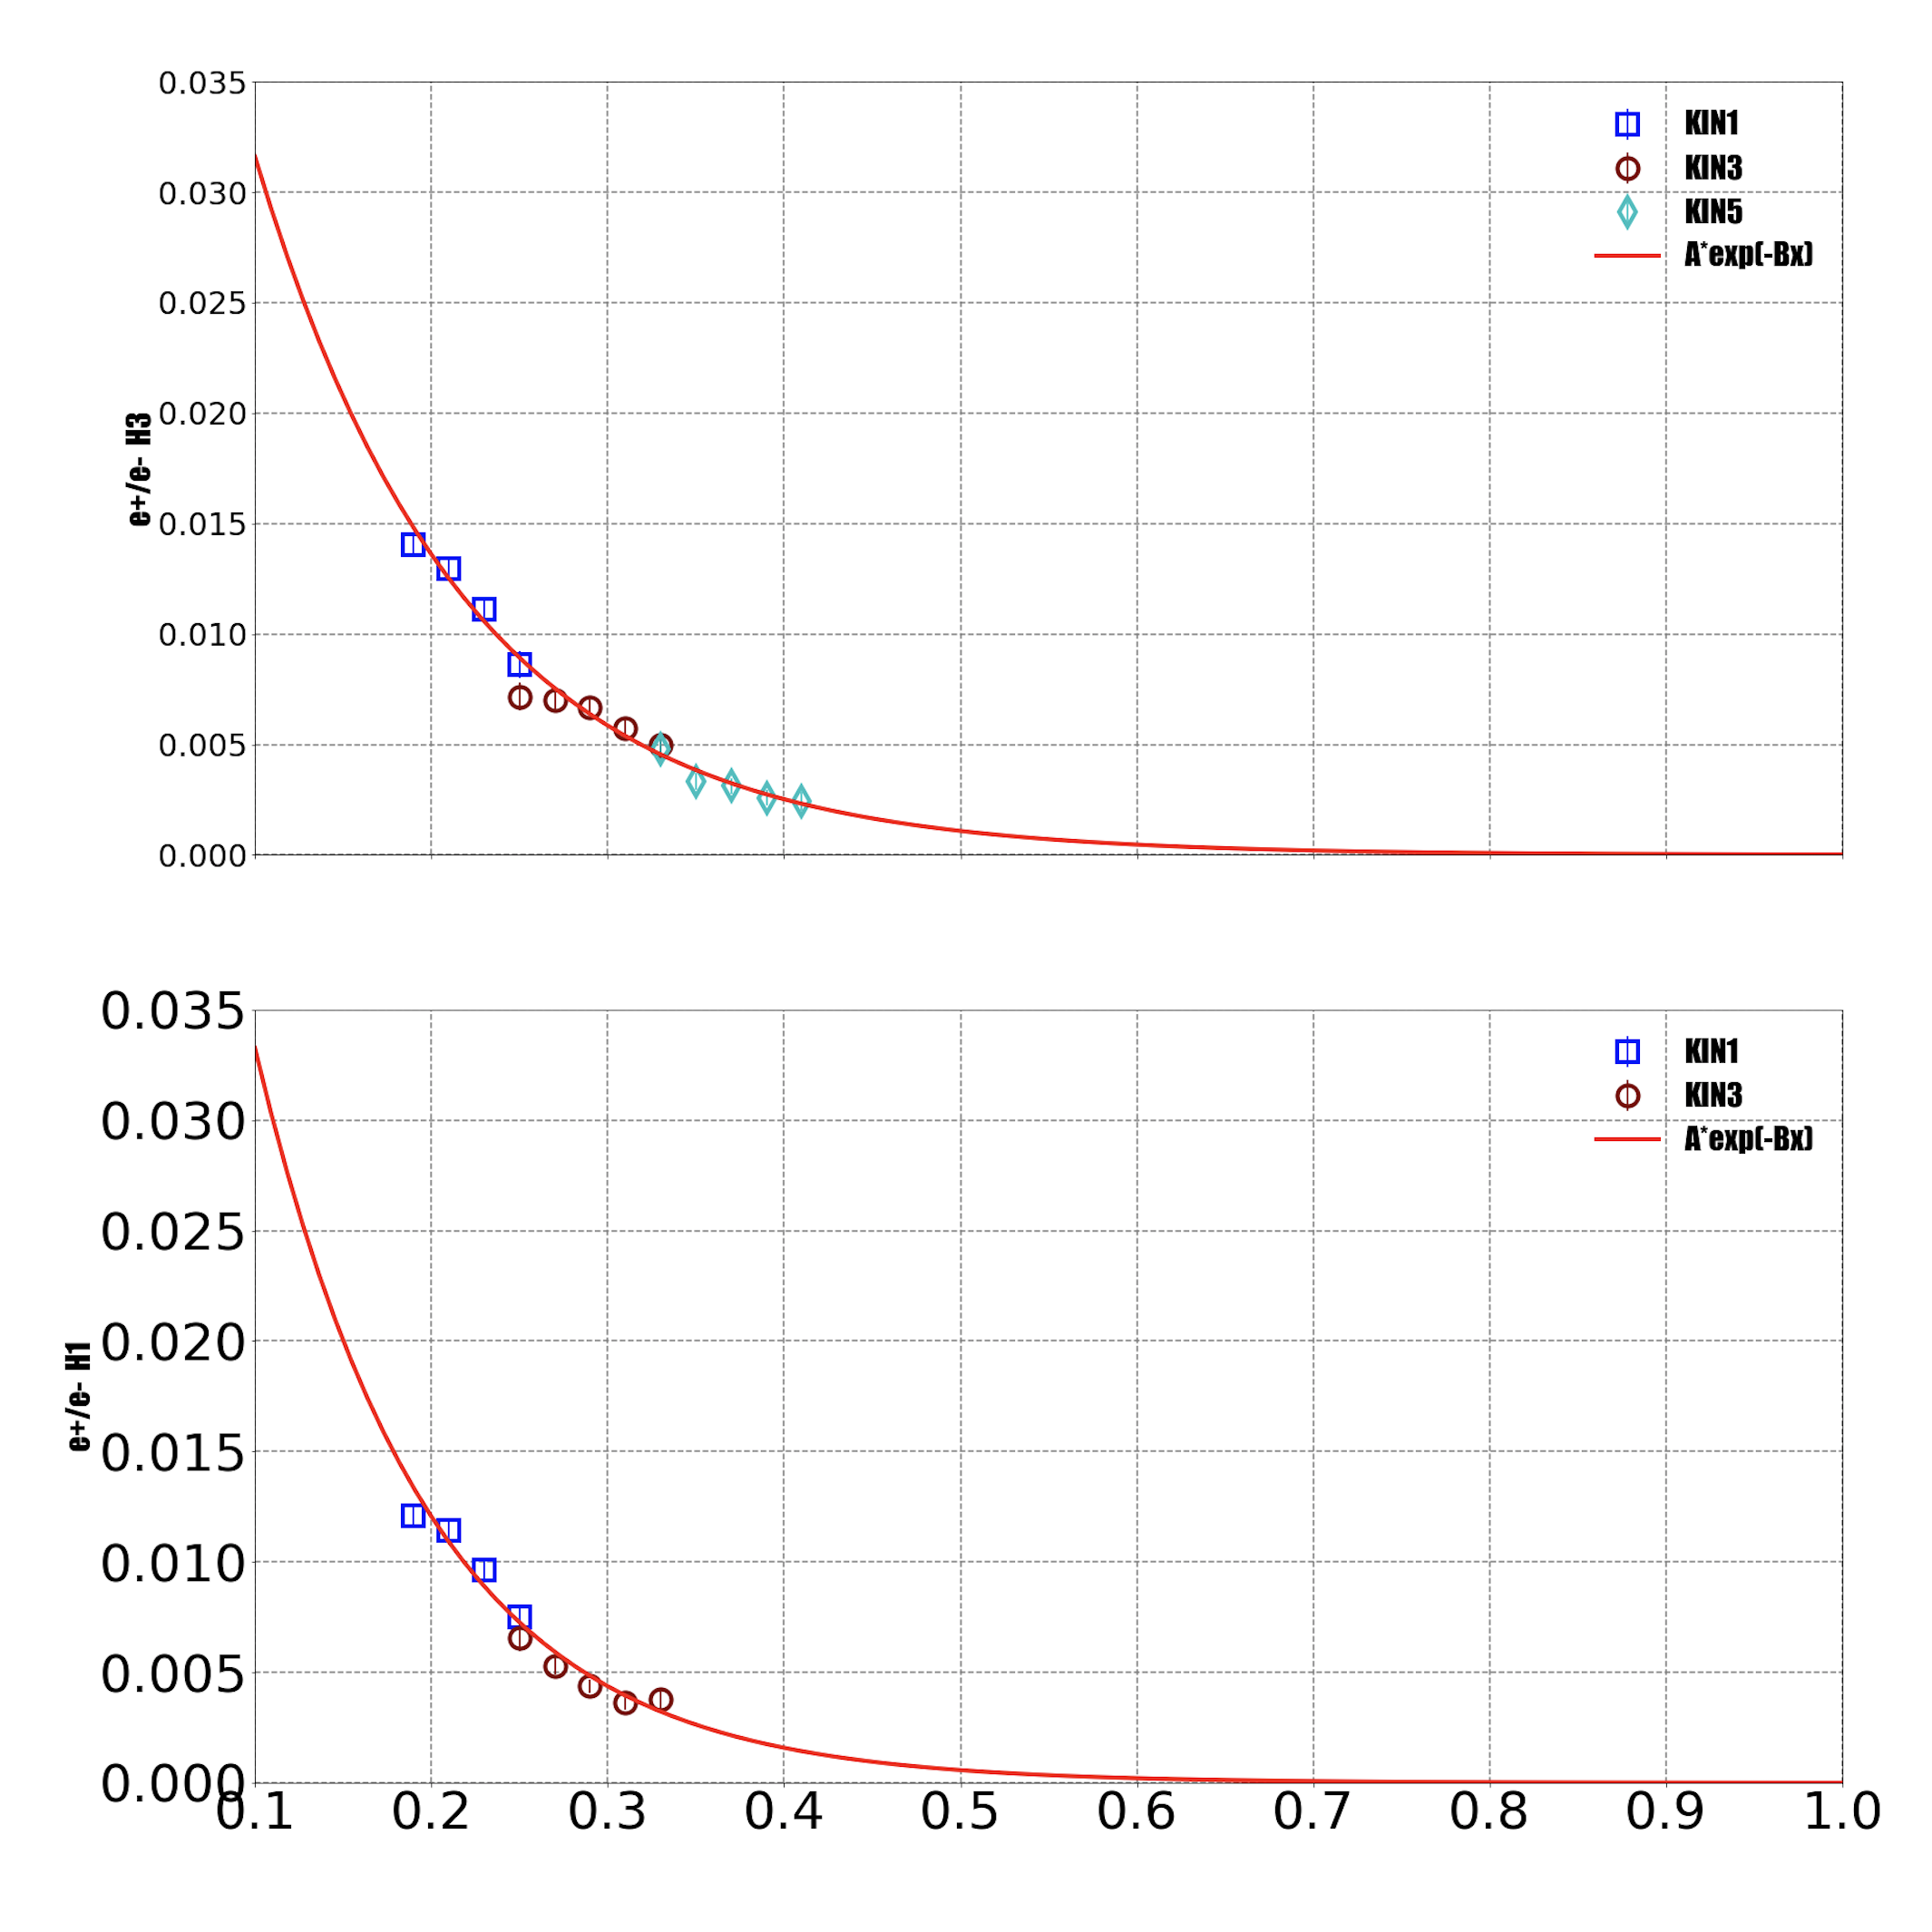
\includegraphics[width=0.4\textwidth] {./Positron_plot/Positron_2.png}
 		\caption{ Fig note : e+/e- for all the $^{1}H$ and $^{3}H$  target .An exponential fitting function is to performed to the data and fitting function is extended to the full Bejuken-x range for MARATHON data. } \label{po_2}
 	\end{center}
\end{figure}   
  
\begin{figure}
 	\begin{center}
 		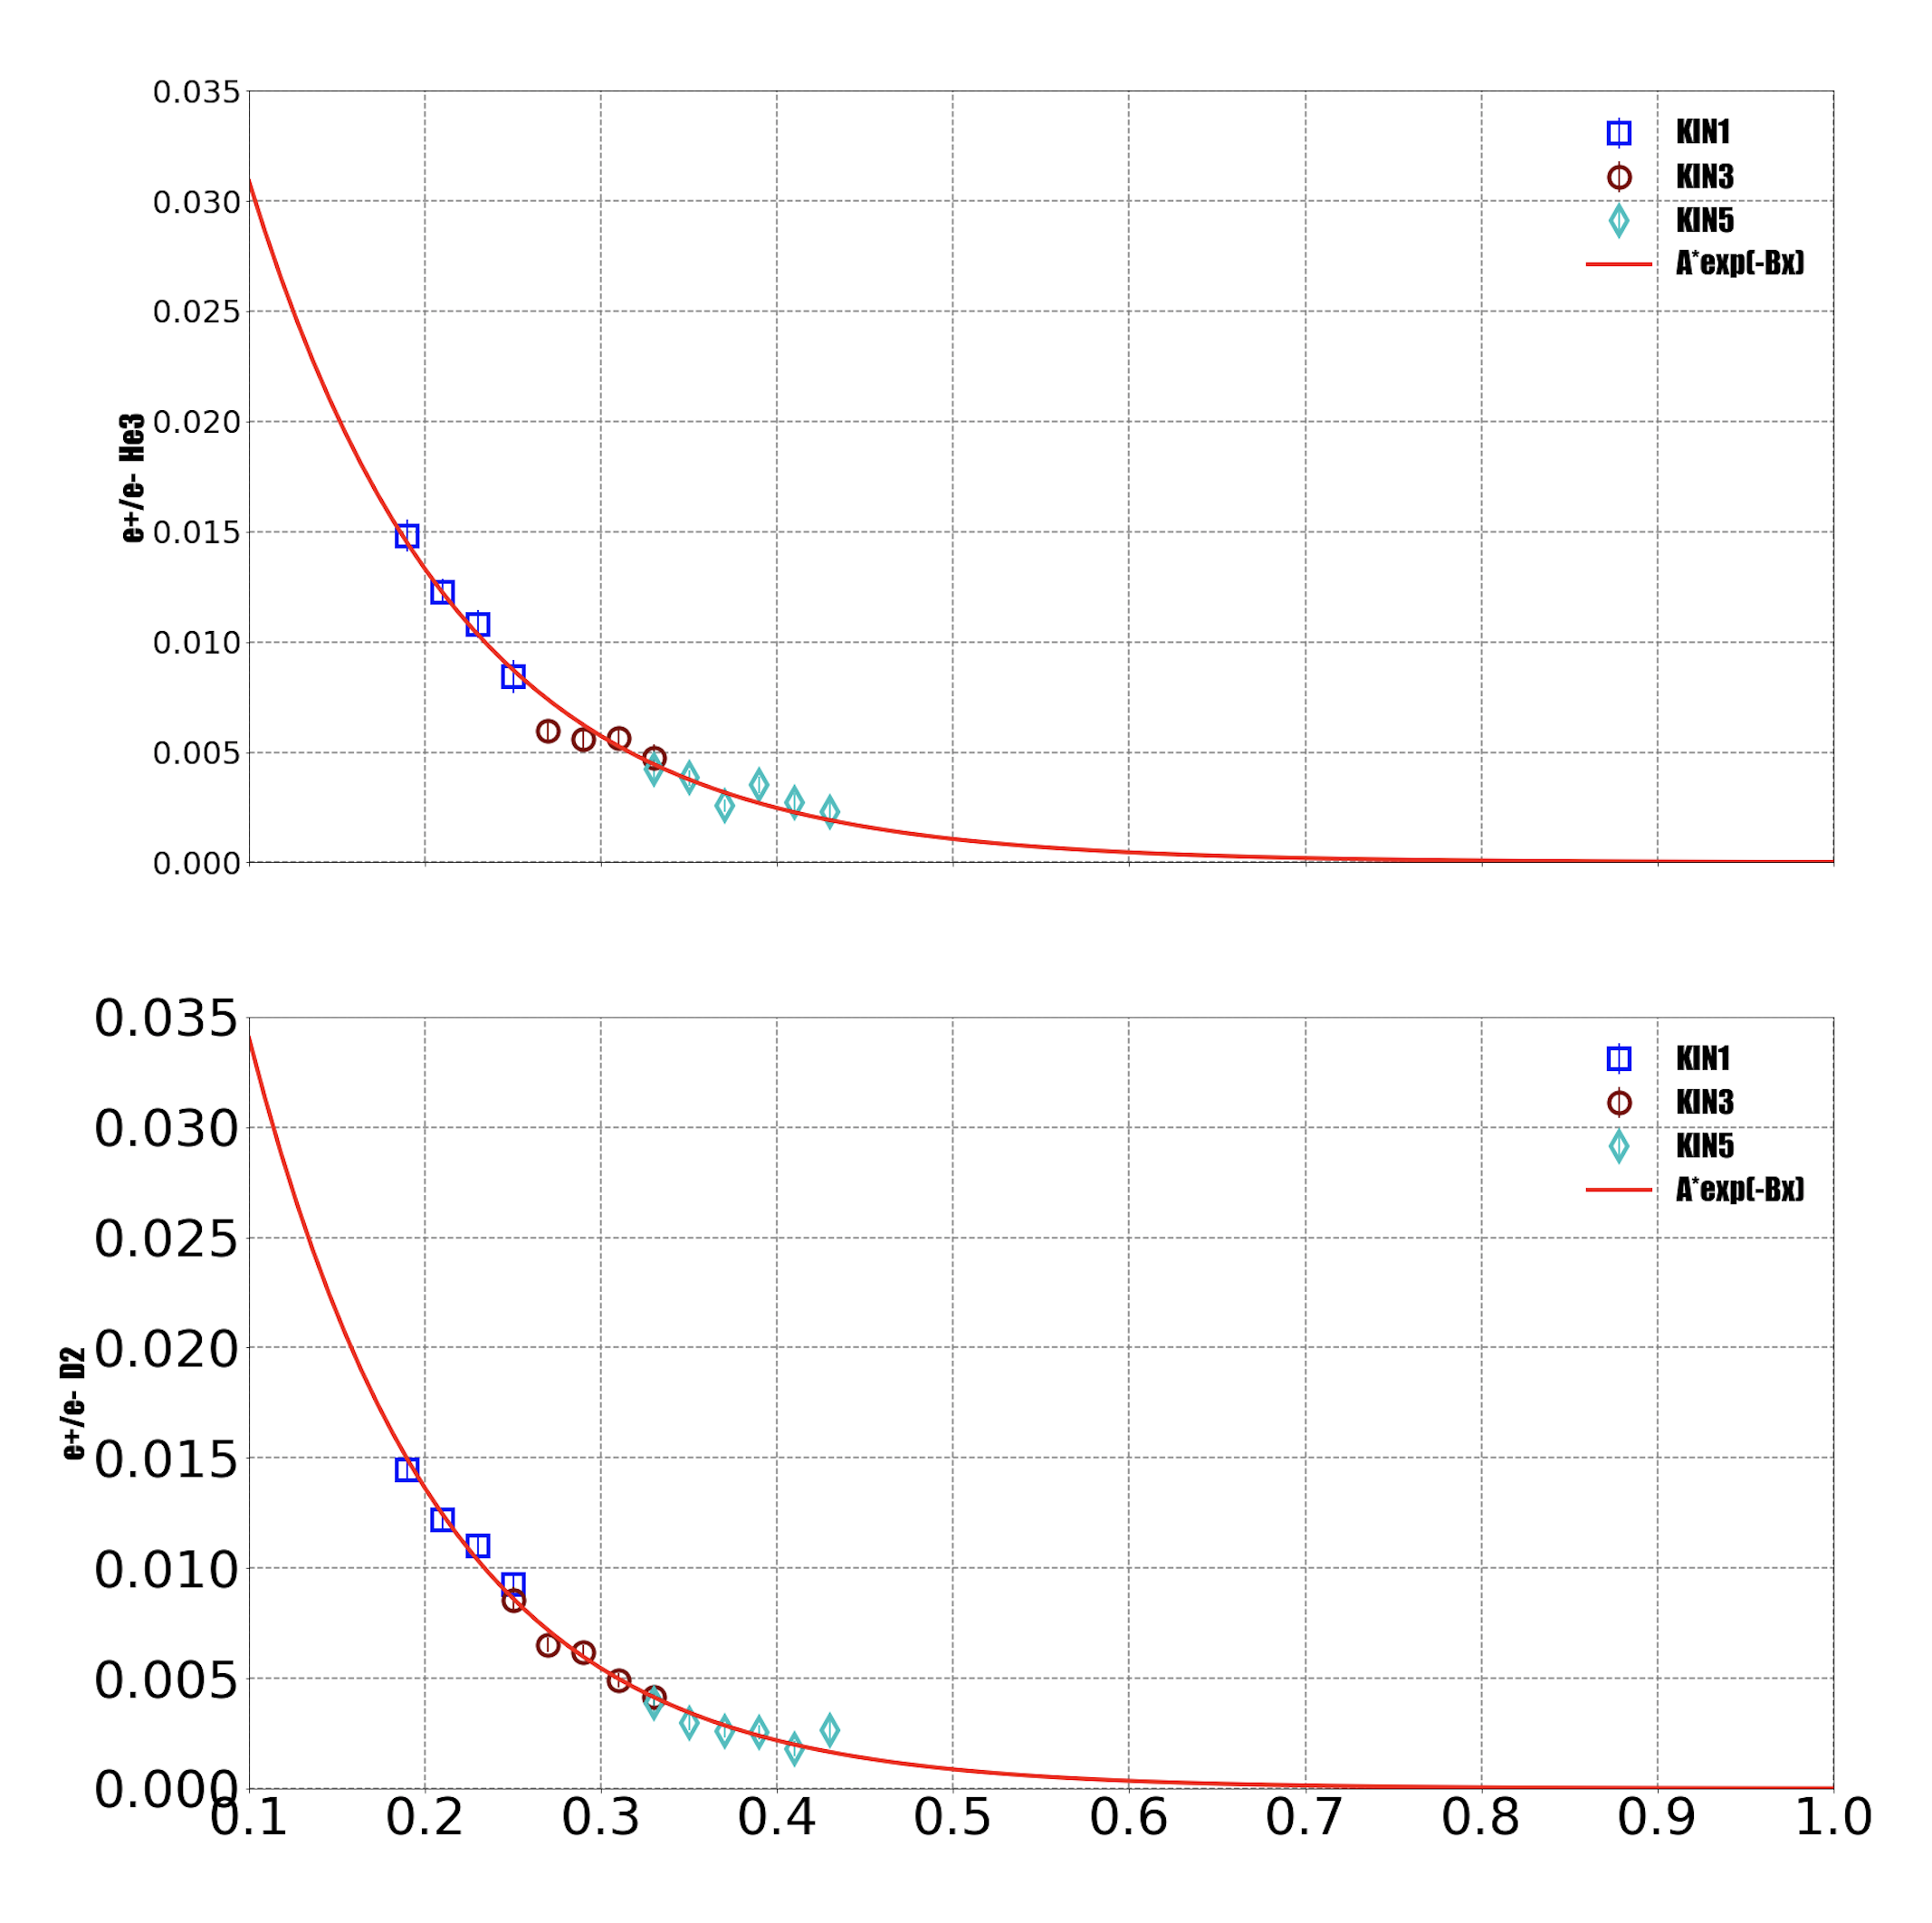
\includegraphics[width=0.4\textwidth] {./Positron_plot/Positron_3.png}
 		\caption{ Fig note : e+/e- for all the $^{3}He$ and $^{2}D$  target .An exponential fitting function is to performed to the data and fitting function is extended to the full Bejuken-x range for MARATHON data. } \label{po_3}
 	\end{center}
\end{figure}  





 \subsection{ii. Endcap Subtraction}
 (Tong Su)

 \subsection{iii. Livetime}

 \subsection{iv. Tritium Decay}
 \subsection{Target composition}

Tritium decays to helium via the $\beta$-decay process $^3\text{H} \,\rightarrow\, ^3\text{He} + e^- + \overline{\nu}_e$, with a half-life of

\begin{equation*}
\tau_{1/2} = \ln(2)\tau = (4500 \pm 8) \text{ days} 
\end{equation*}

This results in a time-dependent target composition, with a decreasing (increasing) population of tritium (helium) nuclei.  These effects must be quantified and corrected in order to accurately extract the normalized tritium yield from tritium target data.

The target cell was filled with an initial tritium number density $n_T^0$, and initial helium number density $n_H^0$.  As tritium decays to helium, these number densities evolve in time as
\begin{align}
n_T &= n_T^0 \: e^{-t/\tau} \label{nT}\\[5pt]
n_H &= n_H^0(1 - e^{-t/\tau}) \label{nH},
\end{align}
where $t$ is the number of days since the target was filled.  Since the decay process preserves the total number of nuclei, the total number density $n_{tot}$ is constant in time:
\begin{align}
n_{tot} 	&= n_T + n_H \nonumber \\
		&= n_T^0 + n_H^0 
\end{align} 

With these quantities, the helium fraction can be defined:
\begin{equation}
f_H = \frac{n_H}{n_T + n_H} = \frac{n_H}{n_{tot}} \label{fH}
\end{equation}
Given an infinite amount of time, all of the tritium will decay to helium.  Therefore $f_H\rightarrow1$ as $t\rightarrow\infty$.  

\subsection{Normalized yield correction}

The normalized yield is defined as:
\begin{equation}
Y = \frac{N}{Qn},
\end{equation}
where $N$ is the number of detected electrons, $Q$ is the beam charge incident on the target, and $n$ is the target number density.  Assume that $N$ includes all corrections (deadtime, efficiency, endcap contamination, etc.) \textit{not} related to tritium decay.  In practice, the yield is extracted from multiple runs, so the number of detected electrons and luminosity must be summed over run number $i$:
\begin{equation}
Y = \frac{\sum N_i}{\sum Q_i n_i},
\end{equation}

The required correction must account not only for the evolution of the target composition (quantified in the previous section), but also for the fact that some of the detected electrons $N$ will have actually scattered from a helium nucleus instead of a tritium nucleus.  Begin by expressing the raw, uncorrected normalized yield (which is measured) as

\begin{equation}
Y_{raw} = \frac{\sum (T_i + H_i)}{\sum Q_i (n_{T,i} + n_{H,i})} \label{Yraw}
\end{equation}
where $T$ and $H$ are the number of detected electrons scattered by tritium and helium, respectively.  For time-dependent quantities (such as $n_{T,i}$ and $n_{H,i}$, given by Equations \ref{nT} and \ref{nH}), the subscript indicates the value of the quantity at the time of run $i$.  The goal is to obtain the normalized tritium yield $Y_T$ in terms of $Y_{raw}$ and correction factors, where

\begin{equation}
Y_T = \frac{\sum T_i}{\sum Q_i n_{T,i}}. 
\end{equation} 

Due to the helium contamination, the correction factor will depend on the normalized helium yield

\begin{equation}
Y_H = \frac{\sum H_i}{\sum Q_i n_{H,i}}. 
\end{equation}

From equation (\ref{Yraw}), only a few steps of algebra are required to obtain $Y_T$.  Recall that the total number density $n_{tot}=n_T + n_H$ is constant in time, and note that the tritium fraction $n_{T,i}/n = 1 - f_{H,i}$, where $f_H$ is the helium fraction defined by Equation \ref{fH}.

\begin{align*}
Y_{raw} 	&= \frac{\sum (T_i + H_i)}{\sum Q_i (n_{T,i} + n_{H,i})} \\[15pt]
		&= \frac{\sum T_i}{n_{tot} \sum Q_i} + \frac{\sum H_i}{n_{tot} \sum Q_i} \\[15pt]
		&= \left(\frac{\sum_i T_i}{\sum_i Q_i n_{T,i}}\right)\left(\frac{\sum_i Q_i n_{T,i}}{n_{tot} \sum_i Q_i}\right)
		+ \left(\frac{\sum_i H_i}{\sum_i Q_i n_{H,i}}\right)\left(\frac{\sum_i Q_i n_{H,i}}{n_{tot} \sum_i Q_i}\right) \\[15pt]
		&= Y_T\left(\frac{\sum Q_i(1-f_{H,i})}{\sum Q_i}\right) + Y_H\left(\frac{\sum Q_i f_{H,i}}{\sum Q_i}\right)
\end{align*}

To simplify notation, define the charge-averaged helium fraction:

\begin{equation}
\langle f_H \rangle \equiv \frac{\sum Q_i f_{H,i}}{\sum Q_i}
\end{equation}

Thus,

\begin{equation}
Y_{raw} = Y_T(1-\langle f_H \rangle) + Y_H \langle f_H \rangle,
\end{equation}

and finally,

\begin{equation}
Y_T = Y_{raw}\left(\frac{1}{1-\langle f_H \rangle}\right) - Y_H \left(\frac{\langle f_H \rangle}{1-\langle f_H \rangle}\right)
\end{equation}

\subsection{Uncertainty propagation}

Pending



 \subsection{v. Boiling}
 (Tong, Mike)

When the beam pass though the target material, the incident electrons can deposit energy in form of heat in the target. This energy deposit can introduce the target boiling along the path of the beam and can also effect the local density of the target.  Since the target boiling effect depends on the thermal property of the target itself and the beam current, a current scan for all the gas targets is a good way to study the densities fluctuation. For MARATHON target cells, three sets of the boiling data were taken. The first set of data is taken at the Dec, 2017 with all four gas targets and also the dummy target and carbon foil as a reference with 5 different currents various form 5uA to 22.5uA. The second set of data was taken at the March of the 2018 with also all 4 gas target but only with 3 different currents. The third set of data was taken at the May 2018, which only cover the tritium and helium target with also 5 different currents.

\begin{table}[h]
\centering
\small
 \caption{Available Boiling Data for the MARATHON Experiment }\label{tab:tablenotes}
\begin{tabular}[t]{|c|c|c|}\hline
 Time & Target & Current  \\ \hline        
  \multirow{4}*{Dec,2017} & Tritium &   2.5$\mu A$/5 $\mu A$/10$\mu A$/15$\mu A$/22.5$\mu A$  \\ 
  \cline{2-3}
         &Helium-3                 &  2.5$\mu A$/5 $\mu A$/10$\mu A$/15$\mu A$/22.5$\mu A$  \\  \cline{2-3}
 & Deuterium                  & 2.5$\mu A$/5 $\mu A$/10$\mu A$/15$\mu A$/22.5$\mu A$   \\  \cline{2-3}
 & Hydrogen                  & 2.5$\mu A$/5 $\mu A$/10$\mu A$/15$\mu A$/22.5$\mu A$  \\  \hline
  \multirow{4}*{March,2018} & Tritium &   11$\mu A$/15 $\mu A$/22.5$\mu A$  \\ 
  \cline{2-3}
         &Helium-3                 &  11$\mu A$/15 $\mu A$/22.5$\mu A$  \\  \cline{2-3}
 & Deuterium                  & 11$\mu A$/15 $\mu A$/22.5$\mu A$  \\  \cline{2-3}
 & Hydrogen                  & 11$\mu A$/15 $\mu A$/22.5$\mu A$ \\  \hline
 \multirow{2}*{March,2017} & Tritium &   2.5$\mu A$/5 $\mu A$/10$\mu A$/15$\mu A$/22.5$\mu A$  \\ 
  \cline{2-3}
         &Helium-3                 &  2.5$\mu A$/5 $\mu A$/10$\mu A$/15$\mu A$/22.5$\mu A$  \\  \hline
 
 
 \end{tabular}
\label{boiling_1} 
 \end{table}

Since the boiling effect is most significant systematic correction for MARATHON data, two independent methods were approach to analyze the boiling effect and both these analysis get the pretty similar result.

The first method is base on to calculate the charge normalized yield with different currents
\begin{equation}  
Yiled=\dfrac{Ne}{C*LT*eff}
\end{equation} 
Where the $C$ is the charge,$LT$ is the live time and $eff$ is the detector efficiency. Since this yield will depends on the target density, so the variation of this yield can reflect the change of the target density with current. Therefore if we normalized this yiled to I=0 ,we can get the how target density can change with different current.
The second method is based on the assumption which also approved by our data that compare the boiling effect of the gas target, the boiling effect of the solid target is ignorable. For each individual target, if we choose the upstream endcap as a reference, we have 
\begin{equation}  
dY=\dfrac{Y_{gas}}{Y_{EndCap}}=\dfrac{N_{gas}}{N_{EndCap}}
\end{equation}   
 
where the $N_{gas}$($N_{EndCap}$) and $Y_{gas}$($Y_{EndCap}$) stand for the number of scattering electrons and the yield from the gas(upstream EndCap). Since the $Y_{EndCap}$ is not changed with current , so if we normalize this ratio to I=0, it can represent how the target density change with different beam current. The advantage for this method is that we do not need to consider the dead time and detector efficiency and beam charge since both of the $Y_{gas}$ ahd $Y_{EndCap}$ comes form the same run ,so all these factors can be canceled from the ratio
The analysisresult of the target boiling effect is shown in the Fig \ref{boiling_plot1}. A quadric fitting function is applied to the combined results for all sets of data and individual target and with this fitting, the target density for different current can be expressed as 
\begin{equation}  
\dfrac{\Delta \rho}{\rho}=p_{0}+p_{1}I+p_{2}I^{2}
\end{equation}  
Where $\rho$ is the target density and $I$ is the beam on current


\begin{figure}[htpb]

\subfigure[Boiling Effect for $^{3}H$]{
\begin{minipage}[t]{1\linewidth}

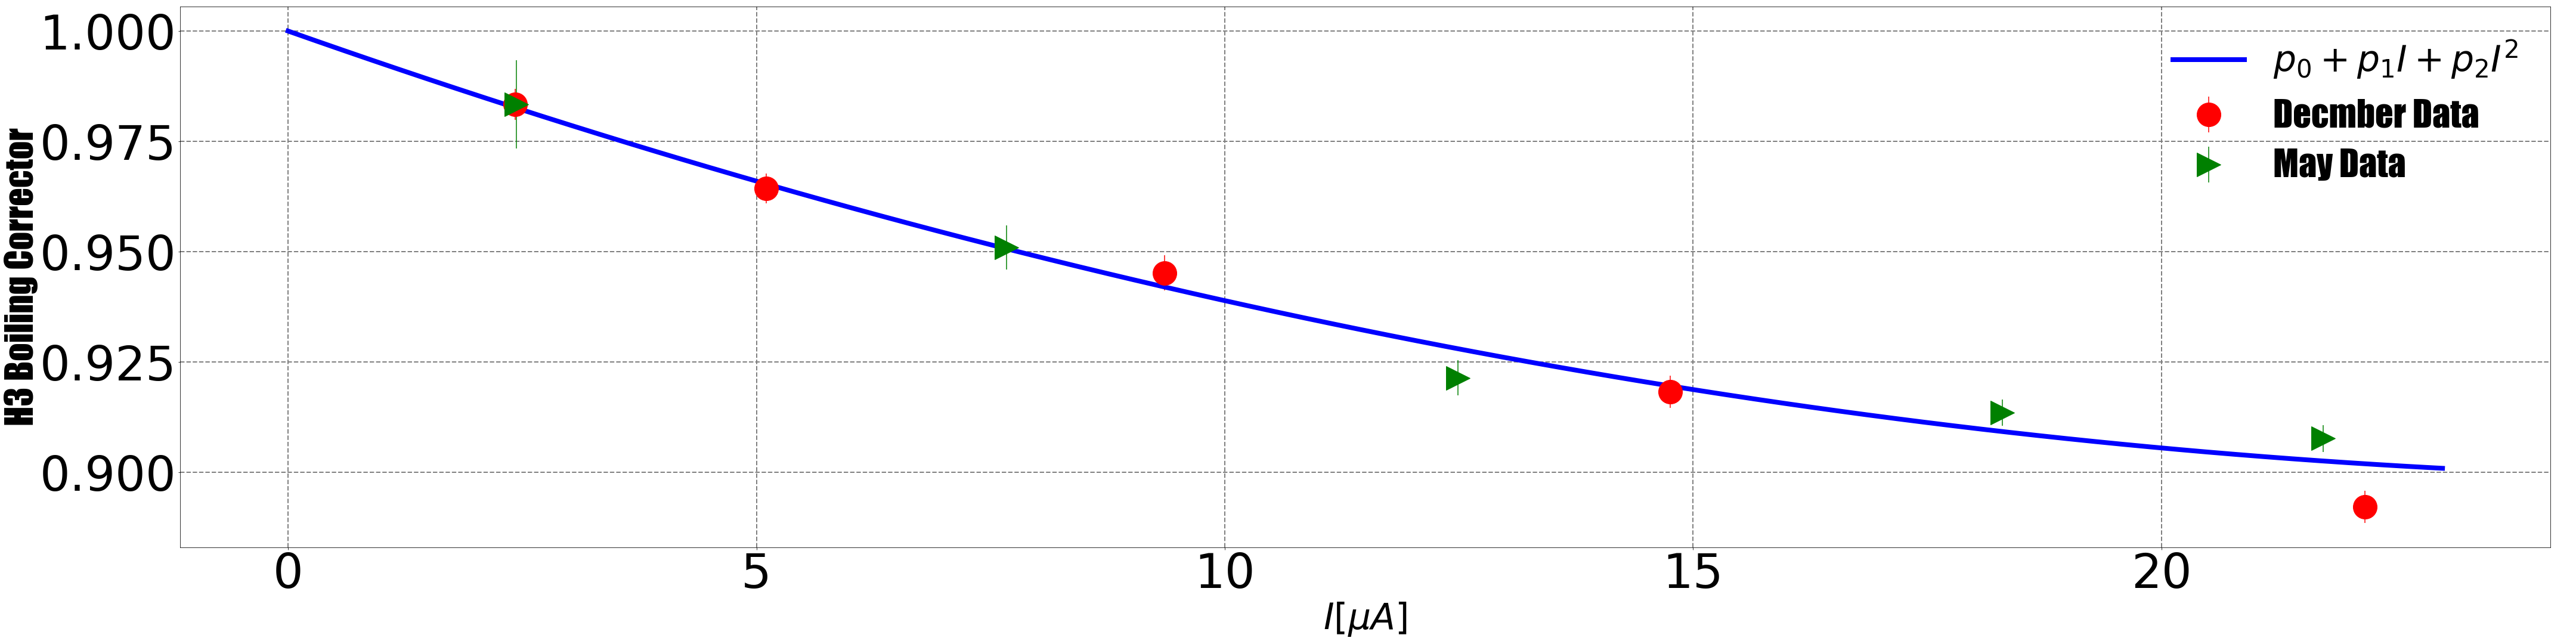
\includegraphics[width=3in]{./boiling_plot/Boiling_H3.png}
\end{minipage}
}\\
\subfigure[Boiling Effect the $^{3}He$]{
\begin{minipage}[t]{1\linewidth}

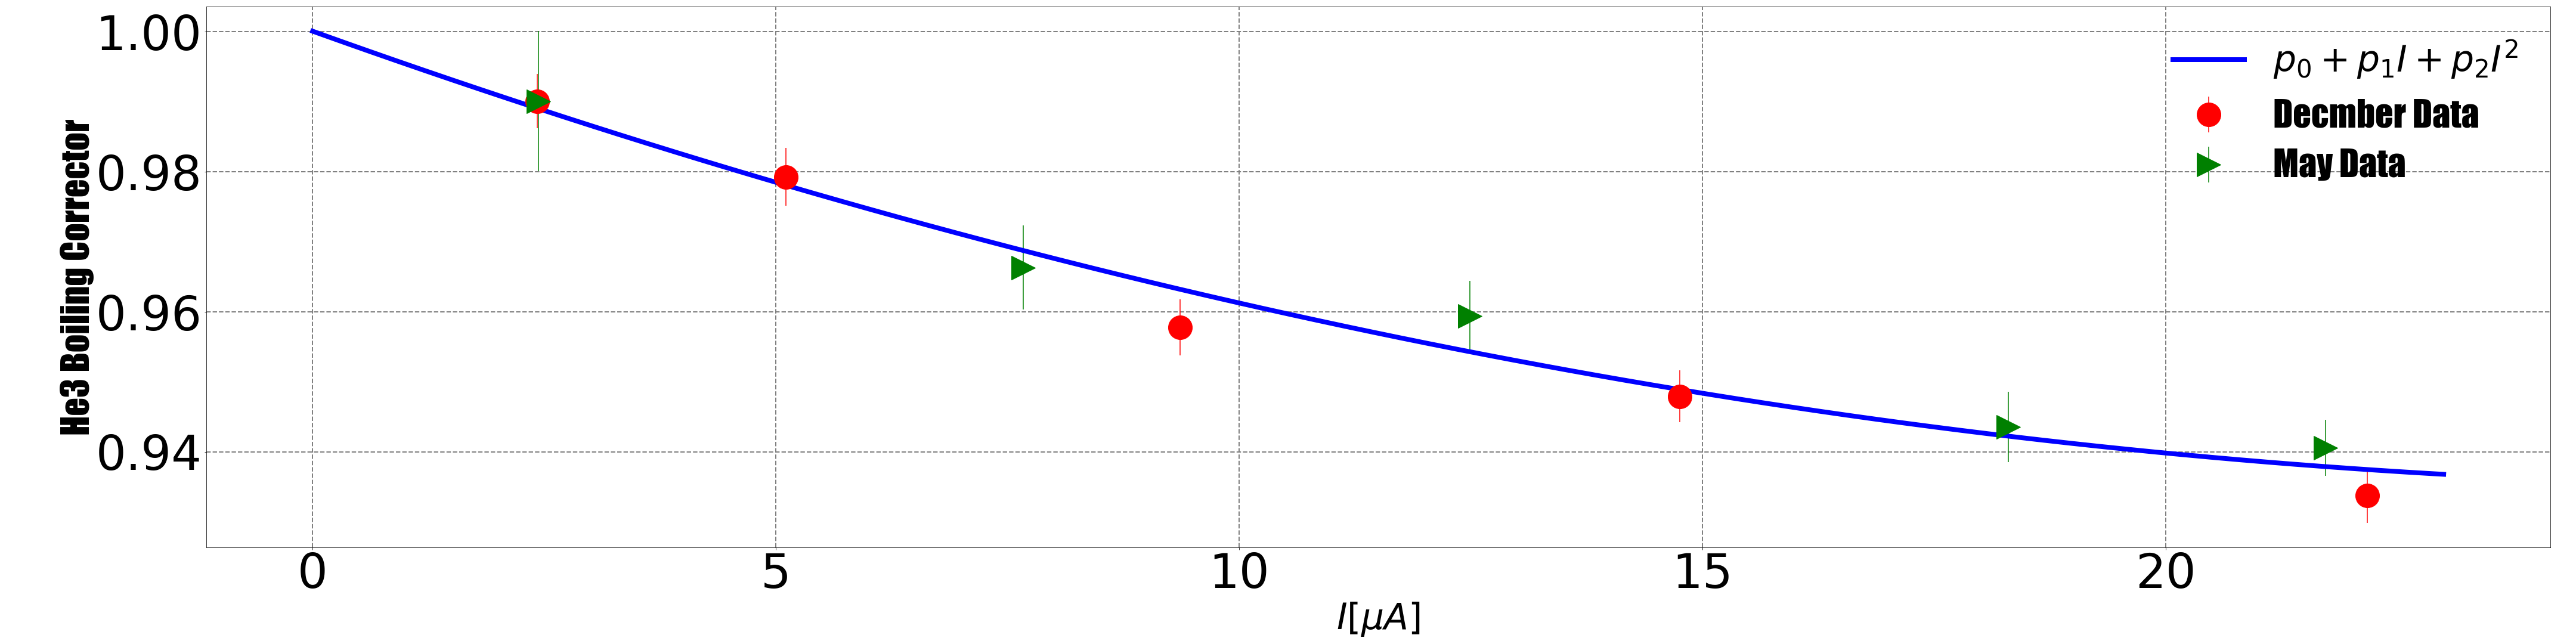
\includegraphics[width=3in]{./boiling_plot/Boiling_He3.png}
\end{minipage}
}

\caption{ the gas target density corrector due to the boiling can be representing equivalently by two ways: Normalized Yield (May Data) or the Normalized Yield ratio(Dec data). The correctors form both methods are shown in the plot and the results agree with each other. For both method, endcap contamination has been taken into consideration and only statistic error is included in the plot  }  \label{boiling_plot1}
\end{figure}

 \subsection{vi. Radiative Corrections}
 (Hanjie Liu)

\section{V. Binning and Combining}

 \subsection{Bin width Choice}

 \subsection{Bin Centering}

 \subsection{Combining Kinematic Overlap}

\end{document}

